%\documentclass[10pt,twocolumn,letterpaper]{article}
\documentclass[runningheads]{llncs}
\usepackage[width=122mm,left=12mm,paperwidth=146mm,height=193mm,top=12mm,paperheight=217mm]{geometry}

\usepackage[tocindentauto]{tocstyle}
% \usepackage{cvpr-ruler-l}
% 
%%%%%%%%%%%%%%%%%%%%%%%%%%%%%%%%%%%%%%%%%%%%%%%%
% Include other packages here, before hyperref.
\usepackage{etex}
\usepackage{url}
\usepackage[numbers]{natbib}
\renewcommand\bibname{References}
\usepackage{cvpr-abbriv}
%%%%
\usepackage{epsfig}
%\usepackage{adjustbox}
\usepackage{graphicx}
\usepackage{amsmath}
\usepackage{amssymb}
\usepackage{array}
\usepackage{tabularx}
\usepackage{url}
\usepackage{graphicx}
\usepackage{amsmath,amssymb} % define this before the line numbering.
%%%%Undefine llncs proof
\makeatletter
\let\lncsproof\proof                         % make \IEEEproof do same as \proof
\let\lncsendproof\endproof              % make \IEEEendproof do same as \endproof
\let\proof\@undefined                        % undefine \proof
\let\endproof\@undefined                  % undefine \endproof
\makeatother
%%%%%%%%%%%%%%
\usepackage{amsthm}
%%%%%%%%%%%%%%
\usepackage{amsthm}
\usepackage{amsxtra}
\usepackage{stmaryrd}
\usepackage{comment}
\usepackage[ruled,vlined,linesnumbered,procnumbered,longend]{algorithm2e}
\newcommand\mycommfont[1]{\small\ttfamily\textcolor{blue}{#1}}
\SetCommentSty{mycommfont}
%
\usepackage{multirow,rotating}
\usepackage{array}
\usepackage{afterpage}
\usepackage{dblfloatfix}
\usepackage{setspace}
\usepackage{floatrow}
\usepackage{booktabs}
\usepackage{color, colortbl}
\usepackage{tabularx,calc}
\usepackage{tikz}                 % create images using pgf/tikz
%\usepackage{subfigure}
\usetikzlibrary{patterns,fit,external}
\usepackage{pgfplots}             % draw plots in tikz style
%\pgfplotsset{compat=1.10}
\usepackage{overpic}
\usepackage{tocloft}
\usepackage{bbm}
%\usepackage{longtable}
\usepackage[absolute]{textpos}
\usepackage{atbeginend}
%\usepackage{enumitem}
%\usepackage{accents}
\usepackage{units}
\usepackage{xifthen}

%\usepackage[titletoc,title]{appendix}

%%%%%%%%%%%%%%%%%%%%%%%%%%%%%%%%%%%%%%%%%%%%%%%%%%%%%%%%%
\usepackage{times}
\usepackage{tikzscale}
\usepackage{marginnote}
\tikzexternalize[prefix=pics_auto/] %activate!
%--------------------------------------
%    TODO Notes
%--------------------------------------
\usepackage[textwidth=2cm,figwidth=\columnwidth,colorinlistoftodos]{todonotes}
% The following hack is to ensure, that tikz externalize does not render todonotes!
\makeatletter
\renewcommand{\todo}[2][]{\tikzexternaldisable\@todo[#1]{#2}\tikzexternalenable}
% \renewcommand{\missingfigure}[2][]{\tikzexternaldisable\@missingfigure[#1]{#2}\tikzexternalenable}
\makeatother
\newcommand{\insertfigure}[2][]{\tikzexternaldisable
\begin{figure}
 \missingfigure[#1]{#2}
 \caption{#2}
\end{figure}
\tikzexternalenable}
\newcommand{\insertref}[1]{\todo[fancyline,color=green!20]{Add reference: #1}}
\newcommand{\explainindetail}[1]{\todo[fancyline,color=red!20]{#1}}
\newcommand{\inlinetodo}[1]{\todo[inline,color=blue!20]{#1}}

\newcounter{mycomment} % Usage:  \mycomment[CR]{Schreib was gscheits}
\newcommand{\mycomment}[2][]
{%
  % initials of the author (optional) + note in the margin
  \refstepcounter{mycomment}%
  {%
%     \setstretch{0.7}% spacing
    \todo[fancyline,color={red!100!green!33},size=\small]
    {%
      \textbf{Comment [\uppercase{#1}\themycomment]:}~#2
    }%
  }
}

% ------------- Tables stuff ------------------------------------------
\usepackage{booktabs}
\usepackage{multirow}
\usepackage{tabularx}
\usepackage{array}
\usepackage{floatrow}
\floatsetup[figure]{style=plain,subcapbesideposition=center}
\usepackage[
  position=bottom,
  font=small,
  labelfont={bf},
%   format=hang,
%   indention=0mm,
]{caption,subfig}
\usepackage{longtable}
\usepackage{tabu} %% !!! this is better!
%%%%%%%%%%%%%%%%%%%%%%%%%%%%Color boxes%%%%%%%%%%%%%%%%%%%%%%%%%%%%%%%%%%%
\usepackage[most]{tcolorbox}
\usepackage{pbox}
\newlength{\luw}
\newlength{\luh}
\newcommand{\flabels}[1]{%
    \settowidth{\luw}{\begin{tabular}{l}\,#1\,\end{tabular}}%
		\settototalheight{\luh}{%
		\begin{tcolorbox}[width=\luw+5pt, boxsep=1pt, left=0pt, right=0pt, top=0pt, bottom=0pt,nobeforeafter]%
		\begin{tabular}{l}%
		\,#1\,\vphantom{$f^1$fq}%
		\end{tabular}%
		\end{tcolorbox}%
		}%
		\pbox[t][][b]{\textwidth}{%
		\resizebox{!}{0.8\luh}{%
		\begin{tcolorbox}[width=\luw+5pt, boxsep=1pt, left=0pt, right=0pt, top=0pt, bottom=0pt,nobeforeafter]%
		\begin{tabular}{l}%
		\,#1\,\vphantom{$f^1$fq}%
		\end{tabular}%
		\end{tcolorbox}%
		}%
		}%
}%

\newcommand{\labelgraphics}[3][width=0.5\linewidth]{%
%\begin{tabular}{c}
\setlength{\fboxsep}{0pt}%
\tikzset{external/export next=false}%
\begin{tikzpicture}%
  \node[inner sep = 0pt] (a) {\includegraphics[#1]{#2}};
  \node[anchor=north west,inner sep=1pt] at (a.north west) {\flabels{#3}};
\end{tikzpicture}%
%\end{tabular}%
}%


%%%%%%%%%%%%%%%%%%%%%%%%%%%%THIS ORDER IS ESSENTIAL%%%%%%%%%%%%%%%%%%%%%%%
\usepackage[draft=false, pagebackref=false,breaklinks=true,colorlinks,bookmarks=false,pdftex]{hyperref}
\hypersetup{hidelinks,colorlinks=false,linkbordercolor={1 1 1}}
%\usepackage{mathrsfs}
\DeclareMathAlphabet{\mathcalligra}{T1}{calligra}{m}{n}
\DeclareMathAlphabet{\mathantt}{OT1}{antt}{li}{it}
\DeclareMathAlphabet{\mathpzc}{OT1}{pzc}{m}{it}

\DeclareMathOperator{\Path}{path}
\DeclareMathOperator{\aff}{aff}
\DeclareMathOperator{\opt}{opt}
\newcommand{\Argmax}{\mathop{\rm Argmax}}
\newcommand{\argmax}{\mathop{\rm argmax}}
\newcommand{\Argmin}{\mathop{\rm Argmin}}
\newcommand{\argmin}{\mathop{\rm argmin}}
\DeclareMathOperator{\Arg}{Arg}
\DeclareMathOperator{\rank}{rank}
\DeclareMathOperator{\Row}{Row}
\DeclareMathOperator{\sign}{sign}
\DeclareMathOperator{\Col}{Col}
\DeclareMathOperator{\ort}{^{\bot}}
\DeclareMathOperator{\dom}{dom}
\DeclareMathOperator{\ri}{relint}
\DeclareMathOperator{\conv}{conv}
\DeclareMathOperator{\coni}{coni}
\DeclareMathOperator{\Null}{null}
\DeclareMathOperator{\select}{select}

\let\oldemptyset\emptyset
\let\emptyset\varnothing

\newcommand{\<}{\langle}
\renewcommand{\>}{\rangle}
\newcommand{\Mid}{\:\big|\,}
\renewcommand{\mid}{\:|\,}
\newcommand{\bb}{\boldsymbol}

\newcommand{\Real}{\mathbb{R}}
%\newcommand{\WI}{\ensuremath{{\rm WI}(\Lambda,f)}\xspace}
%\newcommand{\SI}{\ensuremath{{\rm SI}(\Lambda,f)}\xspace}
%\newcommand{\WIg}{\ensuremath{{\rm WI}(\Lambda,g)}\xspace}
%\newcommand{\SIg}{\ensuremath{{\rm SI}(\Lambda,g)}\xspace}
%\newcommand{\WIx}[1]{\ensuremath{{\mathbb{W}}(\Lambda,#1)}\xspace}
%\newcommand{\SIx}[1]{\ensuremath{{\mathbb{S}}(\Lambda,#1)}\xspace}
%\newcommand{\WI}{\ensuremath{{\mathbb{W}}(\Lambda,f)}\xspace}
%\newcommand{\SI}{\ensuremath{{\mathbb{S}}(\Lambda,f)}\xspace}
%\newcommand{\WIg}{\ensuremath{{\mathbb{W}}(\Lambda,g)}\xspace}
%\newcommand{\SIg}{\ensuremath{{\mathbb{S}}(\Lambda,g)}\xspace}

\newcommand{\WIx}[1]{\ensuremath{\mathbb{W}_{#1}}\xspace}
\newcommand{\SIx}[1]{\ensuremath{\mathbb{S}_{#1}}\xspace}
\newcommand{\WI}{\WIx{f}}
\newcommand{\SI}{\SIx{f}}
\newcommand{\WIg}{\WIx{g}}
\newcommand{\SIg}{\SIx{f}}


\newcommand{\Natural}{\mathbb{N}}
\newcommand{\bbN}{\mathbb{N}}
\newcommand{\bbZ}{\mathbb{Z}}
\newcommand{\bbQ}{\mathbb{Q}}
\newcommand{\Rationals}{\mathbb{Q}}

\def\bbbone{{\mathchoice {\rm 1\mskip-4mu l} {\rm 1\mskip-4mu l}{\rm 1\mskip-4.5mu l} {\rm 1\mskip-5mu l}}}
\newcommand{\Ind}{\bbbone}
\newcommand{\tab}{{\hphantom{bla}}}
\newcommand{\A}{\mathcal{A}}
\newcommand{\Bool}{\mathbb{B}}
\newcommand{\Boolean}{\mathbb{B}}
\newcommand{\bigU}{\mathbb{U}}
\newcommand{\B}{\mathcal{B}}
\newcommand{\D}{\mathcal{D}}
\def\O{\mathcal{O}}
\newcommand{\F}{\mathcal{F}}
\def\G{\mathcal{G}}
\def\H{\mathcal{H}}
\newcommand{\mF}{\mathcal{F}}
\newcommand{\mP}{\mathcal{P}}
\newcommand{\mC}{\mathcal{C}}
\def\C{\mathcal{C}}
\newcommand{\Literals}{\mathbb{\nLabels}}
\newcommand{\V}{\mathcal{V}}
\newcommand{\I}{\mathcal{I}}
\def\U{\mathcal{U}}
\newcommand{\W}{\mathcal{W}}
\renewcommand{\P}{\mathcal{P}}
\newcommand{\E}{\mathcal{E}}
\DeclareMathOperator{\sym}{sym}
\newcommand{\EE}{\tilde{\E}}
\newcommand{\N}{\mathcal{N}}
\newcommand{\X}{\mathcal{X}}
\newcommand{\Y}{\mathcal{Y}}
\newcommand{\calH}{\mathcal{H}}
\newcommand{\calS}{\mathcal{S}}
\newcommand{\calI}{\mathcal{I}}
\renewcommand{\L}{\mathcal{L}}
\newcommand{\M}{\mathcal{M}}
%\newcommand{\LL}{\bb{\mathcal{L}}}
\newcommand{\LL}{\mathcal{X}}
\newcommand{\Labels}{\X}
\newcommand{\nLabels}{L+1}
%\newcommand{\vect}{\overrightarrow}
%\newcommand{\lvect}{\overleftarrow}
\def\T{^{\mathsf T}}
\newcommand{\st}{\mbox{s.t.\ }}

\newcommand{\bulletpar}{\noindent $\bullet\tab$}
\newcounter{myRomanCounter}
\newcommand*{\RomanItem}[1]{\setcounter{myRomanCounter}{#1}\par\noindent\Roman{myRomanCounter}.\ }
\newcommand*{\RomanNumber}[1]{\setcounter{myRomanCounter}{#1}\Roman{myRomanCounter}}

\providecommand{\Zeta}{\mathcal{Z}}

%\def\etalb{{\itshape \bfseries et al.}}
%\def\etalb{{\itshape et al.}}
\def\etalb{ et al.}
\newcommand{\f}{{E_f}}
\newcommand{\g}{{E_g}}
\newcommand{\h}{{E_h}}
\newcommand{\x}{{x}}
\newcommand{\y}{{y}}
\newcommand{\z}{{z}} 
\newcommand{\w}{{w}}

%\newcommand{\sE}{{\scriptsize \textrm{E}}}
%\newcommand{\sG}{{\scriptsize \textrm{G}}}
%\newcommand{\sH}{{\scriptsize \textrm{H}}}

%\newcommand{\c}{{\scriptstyle \textrm{C}}}
%\newcommand{\sD}{{\scriptstyle \textrm{D}}}
%\newcommand{\sH}{{\scriptstyle \textrm{H}}}


%\newcommand{\c}{\textsc{c}}
%\newcommand{\c}{\textsc{c}}
\def\c{\textsc{c}}
\def\d{\textsc{d}}
\def\h{\textsc{h}}
\def\a{\textsc{a}}
\def\b{\textsc{b}}
\def\j{\textsc{j}}
%\newcommand{\sD}{\textsc{d}}
%\newcommand{\sH}{\textsc{h}}

%\newcommand{\c}{\textsc{j}}
%\newcommand{\sD}{\textsc{k}}
%\newcommand{\sH}{\textsc{h}}

\newcommand{\Esubset}{\stackrel{.}{\subsetneq}}
\newcommand{\Esubseteq}{\stackrel{.}{\subset}}
\newcommand{\Esupset}{\stackrel{.}{\supsetneq}}

\newcommand{\Gsubset}{\stackrel{..}{\subsetneq}}
\newcommand{\Gsupset}{\stackrel{..}{\supsetneq}}


%\newcommand{\sE}{e}
%\newcommand{\sG}{c}
%\newcommand{\sH}{d}

\newcommand{\energy}[1]{{E_{#1}}}
\newcommand{\bc}{{\bf c}}
\newcommand{\bzero}{0}
\newcommand{\bone}{1}
\newcommand{\K}{\mathcal{K}}

\newcommand{\nx}{\overline{x}}
\newcommand{\define}{:=}
\newcommand{\PD}{\mathbb{S}_{++}}
\newcommand{\PSD}{\mathbb{S}_{+}}

\newcommand*{\LB}{\ensuremath{\mathit LB}\xspace}
\newcommand*{\LBtwo}{\ensuremath{\mathit LB2}\xspace}
\newcommand*{\LBtwodual}{\ensuremath{\mathit LB2\mbox{-}dual}\xspace}
\newcommand*{\LP}{\ensuremath{\mathit LP\mbox{-}1}\xspace}
\newcommand*{\LPtwo}{\ensuremath{\mathit LP\mbox{-}2}\xspace}


\newtheorem{Note}{note}

\newtheorem{method}{Method}

\newcommand{\smallL}{{\scriptscriptstyle{\left(\right.}}}
\newcommand{\smallR}{{\scriptscriptstyle{\left.\right)}}}

\renewcommand{\iff}{{\textrm{iff} }}

\newcommand{\VH}{V{\'a}clav Hlav{\'a}{\v c}}
\newcommand{\AS}{Alexander Shekhovtsov}
\newcommand{\TW}{Tom{\'a}{\v s} Werner\xspace}
\newcommand{\IRTC}{International Research and Training Center\\ for Informational Technologies and Systems, Kiev}
\newcommand{\CMP}{Czech Technical University in Prague,\\
    Faculty of Electrical Engineering, Department of Cybernetics\\
    Center for Machine Perception}
\newcommand{\gray}{\color[rgb]{0.5,0.5,0.5}}
\newcommand{\red}{\color[rgb]{1,0,0}}
\newcommand{\green}{\color[rgb]{0,1,0}}
\newcommand{\blue}{\color[rgb]{0,0,1}}

\newlength{\figwidth}
\newlength{\figwidtha}
\newlength{\figwidthb}

%\newcommand*{\mypar}[1]{\paragraph{#1}}
\newcommand*{\mypar}[1]{\par{\normalsize\bf #1}\ }
\renewcommand*{\paragraph}[1]{\par\noindent{\normalsize\bf #1}\,\xspace}

\renewcommand*{\marginpar}[1]{\marginnote{#1}}


\def\mathrlap{\mathpalette\mathrlapinternal} 
\def\mathllap{\mathpalette\mathllapinternal}
\def\mathllapinternal#1#2{\llap{$\mathsurround=0pt#1{#2}$}}
\def\mathrlapinternal#1#2{\rlap{$\mathsurround=0pt#1{#2}$}}

\def\ij{i,j}
\def\ji{j,i}
\DeclareRobustCommand{\ind}[1]{\vphantom{f}_{#1}}
\DeclareRobustCommand{\ind}[1]{(#1)}

\def\leftbb{\mathrlap{[}\hskip1.3pt[}
\def\rightbb{]\hskip1.36pt\mathllap{]}}

\def\bbleft{\leftbb}
\def\bbright{\rightbb}
\def\barvee{\veebar}
\def\Vee{\bigvee}
\def\Wedge{\bigwedge}
\def\phi{\delta}
\def\epsilon{\varepsilon}
\def\eps{\varepsilon}
\newcommand{\IF}{\mbox{ \rm if }}
\newcommand{\OR}{\mbox{ \rm or }}
\newcommand{\AND}{\mbox{ \rm and }}
\newcommand{\OTHERWISE}{\mbox{ \rm otherwise}}
\newcommand{\Algorithm}[1]{{Algorithm\,\ref{#1}}}
\newcommand{\Algorithms}[1]{{Algorithms\,\ref{#1}}}
\newcommand{\Section}[1]{\cref{#1}}
%\newcommand{\Section}[1]{\S\ref{#1}}
\makeatletter
\let\parSym\S
\def\S{\mathcal{S}}
\makeatother
\newcommand{\Figure}[1]{{Figure\,\ref{#1}}}
\newcommand{\Theorem}[1]{{Theorem\,\ref{#1}}}
\newcommand{\Lemma}[1]{{Lemma\,\ref{#1}}}
\newcommand{\Chapter}[1]{{Chapter\,\ref{#1}}}
\newcommand{\Chapters}[1]{{Chapters\,\ref{#1}}}
\newcommand{\Statement}[1]{{Statement\,\ref{#1}}}
\newcommand{\Corollary}[1]{{Corollary\,\ref{#1}}}
\newcommand{\Definition}[1]{{Definition\,\ref{#1}}}

\setlength{\arraycolsep}{0.2em}

\newcommand{\halfskip}{\vskip0.5\baselineskip}
\def\defeq{\buildrel \text{d{}ef}\over =}	
\newcommand{\lsub}[1]{\limits_{\begin{subarray}{l}\setlength{\arraycolsep}{0.2em}#1\end{subarray}}}
\newcommand{\csub}[1]{\limits_{\begin{subarray}{c}\setlength{\arraycolsep}{0.2em}#1\end{subarray}}}
\newcommand{\clim}[1]{\limits_{\begin{subarray}{c}\setlength{\arraycolsep}{0.2em}#1\end{subarray}}}

\newcommand{\mincut}{{\scshape mincut}\xspace}
\newcommand{\maxflow}{{\scshape maxflow}\xspace}
%\newcommand{\mincludegraphics}[2][]{\includegraphics[#1]{#2}}
\makeatletter
\newenvironment{rsmallmatrix}{\null\,\vcenter\bgroup
  \Let@\restore@math@cr\default@tag
  \baselineskip6\ex@ \lineskip1.5\ex@ \lineskiplimit\lineskip
  \ialign\bgroup\hfil$\m@th\scriptstyle##$&&\thickspace\hfil
  $\m@th\scriptstyle##$\crcr
}{
  \crcr\egroup\egroup\,
}
\makeatother
%
\def\maxwi{\eqref{best L-improving}\xspace}
\def\maxsi{{(\mbox{\sc max-si})}\xspace}
\def\cf{\emph{cf}\onedot} \def\Cf{\emph{Cf}\onedot}

%\def\revisit{\ensuremath{\red \triangle}\xspace}
\newcommand{\revisit}[1][]{%
\ifthenelse{\equal{#1}{}}{% no argument
\ensuremath{\red \triangle}\xspace}{%
{\ensuremath{\red \rhd}\xspace}%
{\gray #1}%
{\ensuremath{\red \lhd}\xspace}%
}%
}

\def\anchor [#1]#2{%
\phantomsection{}#1\label{#2}%
\def\arga{#2}%
\global\expandafter\def\csname#2\endcsname{%
\hyperref[#2]{#1}\xspace%
}%
}%

\def\codefunction [#1]#2{%
\phantomsection{}\label{#2}{\ttfamily #1\xspace}%
\def\arga{#2}%
\global\expandafter\def\csname#2\endcsname{%
\hyperref[#2]{\ttfamily #1}\xspace%
}%
}

\usepackage{array}
\newcolumntype{L}[1]{>{\raggedright\let\newline\\\arraybackslash\hspace{0pt}}m{#1}}
\newcolumntype{C}[1]{>{\centering\let\newline\\\arraybackslash\hspace{0pt}}m{#1}}
\newcolumntype{R}[1]{>{\raggedleft\let\newline\\\arraybackslash\hspace{0pt}}m{#1}}

\def\checkmark{\tikz\fill[scale=0.4](0,.35) -- (.25,0) -- (1,.7) -- (.25,.15) -- cycle;}

\newcommand{\mm}{\mathit{m}}

\SetKwFor{forever}{while true}{}{end while}
\def\peq{\mathrel{{+}{=}}}
\def\meq{\mathrel{{-}{=}}}

\newcommand{\ubar}[1]{\underaccent{\bar}{#1}}

\newcommand{\norm}[1]{\lVert#1\rVert_1}

\newcommand{\footlabel}[2]{%
    \addtocounter{footnote}{1}%
    \footnotetext[\thefootnote]{%
        \addtocounter{footnote}{-1}%
        \refstepcounter{footnote}\label{#1}%
        #2%
    }%
    $^{\ref{#1}}$%
}

\newcommand{\footref}[1]{%
    $^{\ref{#1}}$%
}

\def\epsilon{\varepsilon}

\newcommand{\leqL}{\mathbin{{\leq}_{\text{\tiny{L}}}}}
\newcommand{\leqAP}{\mathbin{{\leq}_{\text{\tiny AP}}}}
%\usepackage{atbeginend}
\newlength{\myskip}
\setlength{\myskip}{\baselineskip}
%
\def\skipalgomyskip{\vspace{0\myskip}}
\def\skipmyskip{\vspace{0.5\myskip}}

\renewenvironment{enumerate}%
  {\begin{list}{\arabic{enumi}.}%
     {\topsep=0in\itemsep=0in\parsep=0pt\partopsep=0in\usecounter{enumi}}%
   }{\end{list}}
	
\newcounter{itemi}	

\renewenvironment{itemize}%
  {\begin{list}{$\bullet$}%
     {\topsep=0in\itemsep=0pt\parsep=0pt\partopsep=0in\usecounter{itemi}}%
   }{\end{list}\addvspace{0pt}}

%\newcommand{\sectionskip}{\vspace{0mm}}

\raggedbottom
%%% SPACE squeeze
\topsep=0pt %space between first item and preceding paragraph
\partopsep=0pt %extra space added to \topsep when environment starts a new paragraph.
\itemsep=0pt % space between successive items.
%\parskip=0pt

%\setlength{\headsep}{0pt}
\setlength{\tabcolsep}{0pt}
%\setlength{\topmargin}{0pt}
\arraycolsep = 1.2\arraycolsep
%\topskip = 0pt
\floatsep = 0.7\myskip % space left between floats
%\textfloatsep = 4mm %space between last top float or first bottom float and the text
\setlength{\textfloatsep}{12pt plus 1.0pt}
\setlength{\dbltextfloatsep}{\textfloatsep}
\setlength{\dblfloatsep}{\floatsep}
\intextsep = 5mm %space left on top and bottom of an in-text float.
\raggedbottom
\abovecaptionskip = 0pt
\belowcaptionskip = 0pt
%\parskip=0pt
%\setlength{\parsep}{0pt}
%\setlength{\partopsep}{0pt}
%lists
%\topsep=0pt %space between first item and preceding paragraph
%\partopsep=0pt %extra space added to \topsep when environment starts a new paragraph.
\itemsep=0pt % space between successive items.
%
%ALLOW MANY FIGURES
\renewcommand\floatpagefraction{1}
\renewcommand\topfraction{1}
\renewcommand\bottomfraction{1}
\renewcommand\textfraction{0}   
\setcounter{totalnumber}{50}
\setcounter{topnumber}{50}
\setcounter{bottomnumber}{50}
%%%%
\renewcommand{\textfraction}{0.01}
\renewcommand{\floatpagefraction}{0.99}
\renewcommand{\topfraction}{0.99}
\renewcommand{\bottomfraction}{0.99}
\renewcommand{\dblfloatpagefraction}{0.99}
\renewcommand{\dbltopfraction}{0.99}
\setcounter{totalnumber}{99}
\setcounter{topnumber}{99}
\setcounter{bottomnumber}{99}

%\setlength{\algomargin}{0pt}
\SetAlgoSkip{skipalgomyskip}
\SetAlgoInsideSkip{}
%\setlength{\interspaceboxrule}{0pt}
%\setlength{\interspacetitleruled}{0pt}

%%%%%%%%%%%%%%
\makeatletter
\let\corollary\@undefined
%\let\c@corollary\@undefined
\let\endcorollary\@undefined
\let\definition\@undefined
%\let\c@definition\@undefined
\let\enddefinition\@undefined
\let\proof\@undefined
\let\endproof\@undefined
\let\theorem\@undefined
\let\c@theorem\@undefined
\let\endtheorem\@undefined
\let\lemma\@undefined
%\let\c@lemma\@undefined
\let\endlemma\@undefined
%
\let\example\@undefined
\let\c@example\@undefined
\let\endexample\@undefined
\let\remark\@undefined
%\let\c@remark\@undefined
\let\endremark\@undefined
\let\proposition\@undefined
%\let\c@proposition\@undefined
\let\endproposition\@undefined
\let\property\@undefined
\let\endproperty\@undefined
\makeatother

\usepackage{thmtools}

\newtheoremstyle{tightItalic}% name
  {0.5\myskip}%      Space above
  {0\myskip}%      Space below
  {}%         Body font
  {}%         Indent amount (empty = no indent, \parindent = para indent)
  {\itshape}% Thm head font
  {.}%        Punctuation after thm head
  { }%     Space after thm head: " " = normal interword space;
        %       \newline = linebreak
  {}%         Thm head spec (can be left empty, meaning `normal')

\newtheoremstyle{tightBf}% name
  {0.5\myskip}%      Space above
  {0.5\myskip}%      Space below, 0 since amsart starts a paragraph
  {}%         Body font
  {}%         Indent amount (empty = no indent, \parindent = para indent)
  {\bf}% Thm head font
  {.}%        Punctuation after thm head
  {.5em}%     Space after thm head: " " = normal interword space;
        %       \newline = linebreak
  {}%         Thm head spec (can be left empty, meaning `normal')

\theoremstyle{definition}
\theoremstyle{tightBf}
\declaretheorem[style=tightBf,parent=section]{thm}
\numberwithin{thm}{section}
%\declaretheorem[name=Theorem,style=tightBf,parent=section]{theorem}
\declaretheorem[style=tightBf,sibling=thm,name=Theorem]{theorem}
\declaretheorem[style=tightBf,sibling=theorem,name=Lemma]{lemma}
\declaretheorem[style=tightBf,sibling=theorem,name=Definition]{definition}
\declaretheorem[style=tightBf,sibling=theorem,name=Corollary]{corollary}
\declaretheorem[style=tightBf,sibling=theorem,name=Proposition]{proposition}
\declaretheorem[style=tightBf,sibling=theorem,name=Statement]{statement}
\declaretheorem[style=tightBf,sibling=theorem,name=Fact]{fact}
%
\declaretheorem[style=tightBf,parent=section,name=Example]{example}
\numberwithin{example}{section}

\declaretheorem[style=tightItalic,sibling=theorem,name=Remark]{remark}

%\newtheorem{theorem}{Theorem}[section]
%\numberwithin{theorem}{section}
%\newtheorem*{theorem*}{Theorem}
%%\newtheorem{corollary}[theorem]{Corollary}
%\declaretheorem[sharecounter=theorem]{corollary}{Corollary}
%\newtheorem{definition}[theorem]{Definition}
%\newtheorem*{definition*}{Definition}
%\newtheorem{statement}[theorem]{Statement}
%\newtheorem{lemma}[theorem]{Lemma}
%\newtheorem{example}{Example}
%\numberwithin{example}{section}
%\newtheorem*{remark*}{Remark}
%\newtheorem{remark}[theorem]{Remark}
%\newtheorem{proposition}[theorem]{Proposition}
%\newtheorem*{discussion}{Discussion}
%\newtheorem*{property}{Property}
%\numberwithin{property}{section}


\theoremstyle{tightItalic}
\newtheorem*{proof}{Proof}
\BeforeEnd{proof}{\qed}
\newtheorem*{proofsketch}{Proof Sketch}
%\BeforeEnd{proofsketch}{\qed}
%%
%%section and subsection spacing
%%
%\makeatletter
%\renewcommand\section{\@startsection {section}{1}{\z@}%
%{2\myskip}%
%{2\myskip}%
%{\normalfont\Large\bfseries}}
%
%\renewcommand\subsection{\@startsection {subsection}{2}{\z@}%
%{\myskip}%
%{\myskip}%
%{\flushleft\normalfont\bfseries}}
%\makeatother

%\makeatletter
% \def\@endtheorem{\endtrivlist\@endpefalse }% OLD
%\def\@endtheorem{\endtrivlist}% NEW
%\makeatother

\makeatletter
%\setlength{\@fptop}{0pt}
\setlength{\@fptop}{0pt}
\setlength{\@fpsep}{10pt}
\setlength{\@fpbot}{0pt plus 1fil}
\makeatother

\usepackage{thmtools, thm-restate}
\usepackage[capitalise,nameinlink]{cleveref}
\crefformat{equation}{(#2#1#3)}
%\crefname{section}{\S}{\S}
\crefname{section}{\parSym}{\parSym\parSym}
\Crefname{section}{\parSym}{\parSym\parSym}
%%%%%%%%%%%%%%%%%%%%%%%%%%%%%%%%%%%%%%%%%%%%%%%%%%%%%%%%%%%%%%%%%%%%%%%%%%



% \usepackage{ruler}
% \usepackage{authblk}

% \let\classtableofcontents\tableofcontents%

% \renewcommand{\tableofcontents}{%
%   \begingroup%
%   \xpatchcmd{\chapter}{\thispagestyle{empty}}{}{}{}%
%   \classtableofcontents%
%   \endgroup%
% }

%\usepackage{cvpr}
%\usepackage{times}
%\usepackage{epsfig}
%\usepackage{graphicx}
%\usepackage{amsmath}
%\usepackage{amssymb}

% Include other packages here, before hyperref.
% Add by Martin
%\usepackage{amsthm}
%\usepackage[ruled,vlined,linesnumbered]{algorithm2e}
%%\usepackage{mathrsfs}
\DeclareMathAlphabet{\mathcalligra}{T1}{calligra}{m}{n}
\DeclareMathAlphabet{\mathantt}{OT1}{antt}{li}{it}
\DeclareMathAlphabet{\mathpzc}{OT1}{pzc}{m}{it}

\DeclareMathOperator{\Path}{path}
\DeclareMathOperator{\aff}{aff}
\DeclareMathOperator{\opt}{opt}
\newcommand{\Argmax}{\mathop{\rm Argmax}}
\newcommand{\argmax}{\mathop{\rm argmax}}
\newcommand{\Argmin}{\mathop{\rm Argmin}}
\newcommand{\argmin}{\mathop{\rm argmin}}
\DeclareMathOperator{\Arg}{Arg}
\DeclareMathOperator{\rank}{rank}
\DeclareMathOperator{\Row}{Row}
\DeclareMathOperator{\sign}{sign}
\DeclareMathOperator{\Col}{Col}
\DeclareMathOperator{\ort}{^{\bot}}
\DeclareMathOperator{\dom}{dom}
\DeclareMathOperator{\ri}{relint}
\DeclareMathOperator{\conv}{conv}
\DeclareMathOperator{\coni}{coni}
\DeclareMathOperator{\Null}{null}
\DeclareMathOperator{\select}{select}

\let\oldemptyset\emptyset
\let\emptyset\varnothing

\newcommand{\<}{\langle}
\renewcommand{\>}{\rangle}
\newcommand{\Mid}{\:\big|\,}
\renewcommand{\mid}{\:|\,}
\newcommand{\bb}{\boldsymbol}

\newcommand{\Real}{\mathbb{R}}
%\newcommand{\WI}{\ensuremath{{\rm WI}(\Lambda,f)}\xspace}
%\newcommand{\SI}{\ensuremath{{\rm SI}(\Lambda,f)}\xspace}
%\newcommand{\WIg}{\ensuremath{{\rm WI}(\Lambda,g)}\xspace}
%\newcommand{\SIg}{\ensuremath{{\rm SI}(\Lambda,g)}\xspace}
%\newcommand{\WIx}[1]{\ensuremath{{\mathbb{W}}(\Lambda,#1)}\xspace}
%\newcommand{\SIx}[1]{\ensuremath{{\mathbb{S}}(\Lambda,#1)}\xspace}
%\newcommand{\WI}{\ensuremath{{\mathbb{W}}(\Lambda,f)}\xspace}
%\newcommand{\SI}{\ensuremath{{\mathbb{S}}(\Lambda,f)}\xspace}
%\newcommand{\WIg}{\ensuremath{{\mathbb{W}}(\Lambda,g)}\xspace}
%\newcommand{\SIg}{\ensuremath{{\mathbb{S}}(\Lambda,g)}\xspace}

\newcommand{\WIx}[1]{\ensuremath{\mathbb{W}_{#1}}\xspace}
\newcommand{\SIx}[1]{\ensuremath{\mathbb{S}_{#1}}\xspace}
\newcommand{\WI}{\WIx{f}}
\newcommand{\SI}{\SIx{f}}
\newcommand{\WIg}{\WIx{g}}
\newcommand{\SIg}{\SIx{f}}


\newcommand{\Natural}{\mathbb{N}}
\newcommand{\bbN}{\mathbb{N}}
\newcommand{\bbZ}{\mathbb{Z}}
\newcommand{\bbQ}{\mathbb{Q}}
\newcommand{\Rationals}{\mathbb{Q}}

\def\bbbone{{\mathchoice {\rm 1\mskip-4mu l} {\rm 1\mskip-4mu l}{\rm 1\mskip-4.5mu l} {\rm 1\mskip-5mu l}}}
\newcommand{\Ind}{\bbbone}
\newcommand{\tab}{{\hphantom{bla}}}
\newcommand{\A}{\mathcal{A}}
\newcommand{\Bool}{\mathbb{B}}
\newcommand{\Boolean}{\mathbb{B}}
\newcommand{\bigU}{\mathbb{U}}
\newcommand{\B}{\mathcal{B}}
\newcommand{\D}{\mathcal{D}}
\def\O{\mathcal{O}}
\newcommand{\F}{\mathcal{F}}
\def\G{\mathcal{G}}
\def\H{\mathcal{H}}
\newcommand{\mF}{\mathcal{F}}
\newcommand{\mP}{\mathcal{P}}
\newcommand{\mC}{\mathcal{C}}
\def\C{\mathcal{C}}
\newcommand{\Literals}{\mathbb{\nLabels}}
\newcommand{\V}{\mathcal{V}}
\newcommand{\I}{\mathcal{I}}
\def\U{\mathcal{U}}
\newcommand{\W}{\mathcal{W}}
\renewcommand{\P}{\mathcal{P}}
\newcommand{\E}{\mathcal{E}}
\DeclareMathOperator{\sym}{sym}
\newcommand{\EE}{\tilde{\E}}
\newcommand{\N}{\mathcal{N}}
\newcommand{\X}{\mathcal{X}}
\newcommand{\Y}{\mathcal{Y}}
\newcommand{\calH}{\mathcal{H}}
\newcommand{\calS}{\mathcal{S}}
\newcommand{\calI}{\mathcal{I}}
\renewcommand{\L}{\mathcal{L}}
\newcommand{\M}{\mathcal{M}}
%\newcommand{\LL}{\bb{\mathcal{L}}}
\newcommand{\LL}{\mathcal{X}}
\newcommand{\Labels}{\X}
\newcommand{\nLabels}{L+1}
%\newcommand{\vect}{\overrightarrow}
%\newcommand{\lvect}{\overleftarrow}
\def\T{^{\mathsf T}}
\newcommand{\st}{\mbox{s.t.\ }}

\newcommand{\bulletpar}{\noindent $\bullet\tab$}
\newcounter{myRomanCounter}
\newcommand*{\RomanItem}[1]{\setcounter{myRomanCounter}{#1}\par\noindent\Roman{myRomanCounter}.\ }
\newcommand*{\RomanNumber}[1]{\setcounter{myRomanCounter}{#1}\Roman{myRomanCounter}}

\providecommand{\Zeta}{\mathcal{Z}}

%\def\etalb{{\itshape \bfseries et al.}}
%\def\etalb{{\itshape et al.}}
\def\etalb{ et al.}
\newcommand{\f}{{E_f}}
\newcommand{\g}{{E_g}}
\newcommand{\h}{{E_h}}
\newcommand{\x}{{x}}
\newcommand{\y}{{y}}
\newcommand{\z}{{z}} 
\newcommand{\w}{{w}}

%\newcommand{\sE}{{\scriptsize \textrm{E}}}
%\newcommand{\sG}{{\scriptsize \textrm{G}}}
%\newcommand{\sH}{{\scriptsize \textrm{H}}}

%\newcommand{\c}{{\scriptstyle \textrm{C}}}
%\newcommand{\sD}{{\scriptstyle \textrm{D}}}
%\newcommand{\sH}{{\scriptstyle \textrm{H}}}


%\newcommand{\c}{\textsc{c}}
%\newcommand{\c}{\textsc{c}}
\def\c{\textsc{c}}
\def\d{\textsc{d}}
\def\h{\textsc{h}}
\def\a{\textsc{a}}
\def\b{\textsc{b}}
\def\j{\textsc{j}}
%\newcommand{\sD}{\textsc{d}}
%\newcommand{\sH}{\textsc{h}}

%\newcommand{\c}{\textsc{j}}
%\newcommand{\sD}{\textsc{k}}
%\newcommand{\sH}{\textsc{h}}

\newcommand{\Esubset}{\stackrel{.}{\subsetneq}}
\newcommand{\Esubseteq}{\stackrel{.}{\subset}}
\newcommand{\Esupset}{\stackrel{.}{\supsetneq}}

\newcommand{\Gsubset}{\stackrel{..}{\subsetneq}}
\newcommand{\Gsupset}{\stackrel{..}{\supsetneq}}


%\newcommand{\sE}{e}
%\newcommand{\sG}{c}
%\newcommand{\sH}{d}

\newcommand{\energy}[1]{{E_{#1}}}
\newcommand{\bc}{{\bf c}}
\newcommand{\bzero}{0}
\newcommand{\bone}{1}
\newcommand{\K}{\mathcal{K}}

\newcommand{\nx}{\overline{x}}
\newcommand{\define}{:=}
\newcommand{\PD}{\mathbb{S}_{++}}
\newcommand{\PSD}{\mathbb{S}_{+}}

\newcommand*{\LB}{\ensuremath{\mathit LB}\xspace}
\newcommand*{\LBtwo}{\ensuremath{\mathit LB2}\xspace}
\newcommand*{\LBtwodual}{\ensuremath{\mathit LB2\mbox{-}dual}\xspace}
\newcommand*{\LP}{\ensuremath{\mathit LP\mbox{-}1}\xspace}
\newcommand*{\LPtwo}{\ensuremath{\mathit LP\mbox{-}2}\xspace}


\newtheorem{Note}{note}

\newtheorem{method}{Method}

\newcommand{\smallL}{{\scriptscriptstyle{\left(\right.}}}
\newcommand{\smallR}{{\scriptscriptstyle{\left.\right)}}}

\renewcommand{\iff}{{\textrm{iff} }}

\newcommand{\VH}{V{\'a}clav Hlav{\'a}{\v c}}
\newcommand{\AS}{Alexander Shekhovtsov}
\newcommand{\TW}{Tom{\'a}{\v s} Werner\xspace}
\newcommand{\IRTC}{International Research and Training Center\\ for Informational Technologies and Systems, Kiev}
\newcommand{\CMP}{Czech Technical University in Prague,\\
    Faculty of Electrical Engineering, Department of Cybernetics\\
    Center for Machine Perception}
\newcommand{\gray}{\color[rgb]{0.5,0.5,0.5}}
\newcommand{\red}{\color[rgb]{1,0,0}}
\newcommand{\green}{\color[rgb]{0,1,0}}
\newcommand{\blue}{\color[rgb]{0,0,1}}

\newlength{\figwidth}
\newlength{\figwidtha}
\newlength{\figwidthb}

%\newcommand*{\mypar}[1]{\paragraph{#1}}
\newcommand*{\mypar}[1]{\par{\normalsize\bf #1}\ }
\renewcommand*{\paragraph}[1]{\par\noindent{\normalsize\bf #1}\,\xspace}

\renewcommand*{\marginpar}[1]{\marginnote{#1}}


\def\mathrlap{\mathpalette\mathrlapinternal} 
\def\mathllap{\mathpalette\mathllapinternal}
\def\mathllapinternal#1#2{\llap{$\mathsurround=0pt#1{#2}$}}
\def\mathrlapinternal#1#2{\rlap{$\mathsurround=0pt#1{#2}$}}

\def\ij{i,j}
\def\ji{j,i}
\DeclareRobustCommand{\ind}[1]{\vphantom{f}_{#1}}
\DeclareRobustCommand{\ind}[1]{(#1)}

\def\leftbb{\mathrlap{[}\hskip1.3pt[}
\def\rightbb{]\hskip1.36pt\mathllap{]}}

\def\bbleft{\leftbb}
\def\bbright{\rightbb}
\def\barvee{\veebar}
\def\Vee{\bigvee}
\def\Wedge{\bigwedge}
\def\phi{\delta}
\def\epsilon{\varepsilon}
\def\eps{\varepsilon}
\newcommand{\IF}{\mbox{ \rm if }}
\newcommand{\OR}{\mbox{ \rm or }}
\newcommand{\AND}{\mbox{ \rm and }}
\newcommand{\OTHERWISE}{\mbox{ \rm otherwise}}
\newcommand{\Algorithm}[1]{{Algorithm\,\ref{#1}}}
\newcommand{\Algorithms}[1]{{Algorithms\,\ref{#1}}}
\newcommand{\Section}[1]{\cref{#1}}
%\newcommand{\Section}[1]{\S\ref{#1}}
\makeatletter
\let\parSym\S
\def\S{\mathcal{S}}
\makeatother
\newcommand{\Figure}[1]{{Figure\,\ref{#1}}}
\newcommand{\Theorem}[1]{{Theorem\,\ref{#1}}}
\newcommand{\Lemma}[1]{{Lemma\,\ref{#1}}}
\newcommand{\Chapter}[1]{{Chapter\,\ref{#1}}}
\newcommand{\Chapters}[1]{{Chapters\,\ref{#1}}}
\newcommand{\Statement}[1]{{Statement\,\ref{#1}}}
\newcommand{\Corollary}[1]{{Corollary\,\ref{#1}}}
\newcommand{\Definition}[1]{{Definition\,\ref{#1}}}

\setlength{\arraycolsep}{0.2em}

\newcommand{\halfskip}{\vskip0.5\baselineskip}
\def\defeq{\buildrel \text{d{}ef}\over =}	
\newcommand{\lsub}[1]{\limits_{\begin{subarray}{l}\setlength{\arraycolsep}{0.2em}#1\end{subarray}}}
\newcommand{\csub}[1]{\limits_{\begin{subarray}{c}\setlength{\arraycolsep}{0.2em}#1\end{subarray}}}
\newcommand{\clim}[1]{\limits_{\begin{subarray}{c}\setlength{\arraycolsep}{0.2em}#1\end{subarray}}}

\newcommand{\mincut}{{\scshape mincut}\xspace}
\newcommand{\maxflow}{{\scshape maxflow}\xspace}
%\newcommand{\mincludegraphics}[2][]{\includegraphics[#1]{#2}}
\makeatletter
\newenvironment{rsmallmatrix}{\null\,\vcenter\bgroup
  \Let@\restore@math@cr\default@tag
  \baselineskip6\ex@ \lineskip1.5\ex@ \lineskiplimit\lineskip
  \ialign\bgroup\hfil$\m@th\scriptstyle##$&&\thickspace\hfil
  $\m@th\scriptstyle##$\crcr
}{
  \crcr\egroup\egroup\,
}
\makeatother
%
\def\maxwi{\eqref{best L-improving}\xspace}
\def\maxsi{{(\mbox{\sc max-si})}\xspace}
\def\cf{\emph{cf}\onedot} \def\Cf{\emph{Cf}\onedot}

%\def\revisit{\ensuremath{\red \triangle}\xspace}
\newcommand{\revisit}[1][]{%
\ifthenelse{\equal{#1}{}}{% no argument
\ensuremath{\red \triangle}\xspace}{%
{\ensuremath{\red \rhd}\xspace}%
{\gray #1}%
{\ensuremath{\red \lhd}\xspace}%
}%
}

\def\anchor [#1]#2{%
\phantomsection{}#1\label{#2}%
\def\arga{#2}%
\global\expandafter\def\csname#2\endcsname{%
\hyperref[#2]{#1}\xspace%
}%
}%

\def\codefunction [#1]#2{%
\phantomsection{}\label{#2}{\ttfamily #1\xspace}%
\def\arga{#2}%
\global\expandafter\def\csname#2\endcsname{%
\hyperref[#2]{\ttfamily #1}\xspace%
}%
}

\usepackage{array}
\newcolumntype{L}[1]{>{\raggedright\let\newline\\\arraybackslash\hspace{0pt}}m{#1}}
\newcolumntype{C}[1]{>{\centering\let\newline\\\arraybackslash\hspace{0pt}}m{#1}}
\newcolumntype{R}[1]{>{\raggedleft\let\newline\\\arraybackslash\hspace{0pt}}m{#1}}

\def\checkmark{\tikz\fill[scale=0.4](0,.35) -- (.25,0) -- (1,.7) -- (.25,.15) -- cycle;}

\newcommand{\mm}{\mathit{m}}

\SetKwFor{forever}{while true}{}{end while}
\def\peq{\mathrel{{+}{=}}}
\def\meq{\mathrel{{-}{=}}}

\newcommand{\ubar}[1]{\underaccent{\bar}{#1}}

\newcommand{\norm}[1]{\lVert#1\rVert_1}

\newcommand{\footlabel}[2]{%
    \addtocounter{footnote}{1}%
    \footnotetext[\thefootnote]{%
        \addtocounter{footnote}{-1}%
        \refstepcounter{footnote}\label{#1}%
        #2%
    }%
    $^{\ref{#1}}$%
}

\newcommand{\footref}[1]{%
    $^{\ref{#1}}$%
}

\def\epsilon{\varepsilon}

\newcommand{\leqL}{\mathbin{{\leq}_{\text{\tiny{L}}}}}
\newcommand{\leqAP}{\mathbin{{\leq}_{\text{\tiny AP}}}}
%%\usepackage{atbeginend}
\newlength{\myskip}
\setlength{\myskip}{\baselineskip}
%
\def\skipalgomyskip{\vspace{0\myskip}}
\def\skipmyskip{\vspace{0.5\myskip}}

\renewenvironment{enumerate}%
  {\begin{list}{\arabic{enumi}.}%
     {\topsep=0in\itemsep=0in\parsep=0pt\partopsep=0in\usecounter{enumi}}%
   }{\end{list}}
	
\newcounter{itemi}	

\renewenvironment{itemize}%
  {\begin{list}{$\bullet$}%
     {\topsep=0in\itemsep=0pt\parsep=0pt\partopsep=0in\usecounter{itemi}}%
   }{\end{list}\addvspace{0pt}}

%\newcommand{\sectionskip}{\vspace{0mm}}

\raggedbottom
%%% SPACE squeeze
\topsep=0pt %space between first item and preceding paragraph
\partopsep=0pt %extra space added to \topsep when environment starts a new paragraph.
\itemsep=0pt % space between successive items.
%\parskip=0pt

%\setlength{\headsep}{0pt}
\setlength{\tabcolsep}{0pt}
%\setlength{\topmargin}{0pt}
\arraycolsep = 1.2\arraycolsep
%\topskip = 0pt
\floatsep = 0.7\myskip % space left between floats
%\textfloatsep = 4mm %space between last top float or first bottom float and the text
\setlength{\textfloatsep}{12pt plus 1.0pt}
\setlength{\dbltextfloatsep}{\textfloatsep}
\setlength{\dblfloatsep}{\floatsep}
\intextsep = 5mm %space left on top and bottom of an in-text float.
\raggedbottom
\abovecaptionskip = 0pt
\belowcaptionskip = 0pt
%\parskip=0pt
%\setlength{\parsep}{0pt}
%\setlength{\partopsep}{0pt}
%lists
%\topsep=0pt %space between first item and preceding paragraph
%\partopsep=0pt %extra space added to \topsep when environment starts a new paragraph.
\itemsep=0pt % space between successive items.
%
%ALLOW MANY FIGURES
\renewcommand\floatpagefraction{1}
\renewcommand\topfraction{1}
\renewcommand\bottomfraction{1}
\renewcommand\textfraction{0}   
\setcounter{totalnumber}{50}
\setcounter{topnumber}{50}
\setcounter{bottomnumber}{50}
%%%%
\renewcommand{\textfraction}{0.01}
\renewcommand{\floatpagefraction}{0.99}
\renewcommand{\topfraction}{0.99}
\renewcommand{\bottomfraction}{0.99}
\renewcommand{\dblfloatpagefraction}{0.99}
\renewcommand{\dbltopfraction}{0.99}
\setcounter{totalnumber}{99}
\setcounter{topnumber}{99}
\setcounter{bottomnumber}{99}

%\setlength{\algomargin}{0pt}
\SetAlgoSkip{skipalgomyskip}
\SetAlgoInsideSkip{}
%\setlength{\interspaceboxrule}{0pt}
%\setlength{\interspacetitleruled}{0pt}

%%%%%%%%%%%%%%
\makeatletter
\let\corollary\@undefined
%\let\c@corollary\@undefined
\let\endcorollary\@undefined
\let\definition\@undefined
%\let\c@definition\@undefined
\let\enddefinition\@undefined
\let\proof\@undefined
\let\endproof\@undefined
\let\theorem\@undefined
\let\c@theorem\@undefined
\let\endtheorem\@undefined
\let\lemma\@undefined
%\let\c@lemma\@undefined
\let\endlemma\@undefined
%
\let\example\@undefined
\let\c@example\@undefined
\let\endexample\@undefined
\let\remark\@undefined
%\let\c@remark\@undefined
\let\endremark\@undefined
\let\proposition\@undefined
%\let\c@proposition\@undefined
\let\endproposition\@undefined
\let\property\@undefined
\let\endproperty\@undefined
\makeatother

\usepackage{thmtools}

\newtheoremstyle{tightItalic}% name
  {0.5\myskip}%      Space above
  {0\myskip}%      Space below
  {}%         Body font
  {}%         Indent amount (empty = no indent, \parindent = para indent)
  {\itshape}% Thm head font
  {.}%        Punctuation after thm head
  { }%     Space after thm head: " " = normal interword space;
        %       \newline = linebreak
  {}%         Thm head spec (can be left empty, meaning `normal')

\newtheoremstyle{tightBf}% name
  {0.5\myskip}%      Space above
  {0.5\myskip}%      Space below, 0 since amsart starts a paragraph
  {}%         Body font
  {}%         Indent amount (empty = no indent, \parindent = para indent)
  {\bf}% Thm head font
  {.}%        Punctuation after thm head
  {.5em}%     Space after thm head: " " = normal interword space;
        %       \newline = linebreak
  {}%         Thm head spec (can be left empty, meaning `normal')

\theoremstyle{definition}
\theoremstyle{tightBf}
\declaretheorem[style=tightBf,parent=section]{thm}
\numberwithin{thm}{section}
%\declaretheorem[name=Theorem,style=tightBf,parent=section]{theorem}
\declaretheorem[style=tightBf,sibling=thm,name=Theorem]{theorem}
\declaretheorem[style=tightBf,sibling=theorem,name=Lemma]{lemma}
\declaretheorem[style=tightBf,sibling=theorem,name=Definition]{definition}
\declaretheorem[style=tightBf,sibling=theorem,name=Corollary]{corollary}
\declaretheorem[style=tightBf,sibling=theorem,name=Proposition]{proposition}
\declaretheorem[style=tightBf,sibling=theorem,name=Statement]{statement}
\declaretheorem[style=tightBf,sibling=theorem,name=Fact]{fact}
%
\declaretheorem[style=tightBf,parent=section,name=Example]{example}
\numberwithin{example}{section}

\declaretheorem[style=tightItalic,sibling=theorem,name=Remark]{remark}

%\newtheorem{theorem}{Theorem}[section]
%\numberwithin{theorem}{section}
%\newtheorem*{theorem*}{Theorem}
%%\newtheorem{corollary}[theorem]{Corollary}
%\declaretheorem[sharecounter=theorem]{corollary}{Corollary}
%\newtheorem{definition}[theorem]{Definition}
%\newtheorem*{definition*}{Definition}
%\newtheorem{statement}[theorem]{Statement}
%\newtheorem{lemma}[theorem]{Lemma}
%\newtheorem{example}{Example}
%\numberwithin{example}{section}
%\newtheorem*{remark*}{Remark}
%\newtheorem{remark}[theorem]{Remark}
%\newtheorem{proposition}[theorem]{Proposition}
%\newtheorem*{discussion}{Discussion}
%\newtheorem*{property}{Property}
%\numberwithin{property}{section}


\theoremstyle{tightItalic}
\newtheorem*{proof}{Proof}
\BeforeEnd{proof}{\qed}
\newtheorem*{proofsketch}{Proof Sketch}
%\BeforeEnd{proofsketch}{\qed}
%%
%%section and subsection spacing
%%
%\makeatletter
%\renewcommand\section{\@startsection {section}{1}{\z@}%
%{2\myskip}%
%{2\myskip}%
%{\normalfont\Large\bfseries}}
%
%\renewcommand\subsection{\@startsection {subsection}{2}{\z@}%
%{\myskip}%
%{\myskip}%
%{\flushleft\normalfont\bfseries}}
%\makeatother

%\makeatletter
% \def\@endtheorem{\endtrivlist\@endpefalse }% OLD
%\def\@endtheorem{\endtrivlist}% NEW
%\makeatother

\makeatletter
%\setlength{\@fptop}{0pt}
\setlength{\@fptop}{0pt}
\setlength{\@fpsep}{10pt}
\setlength{\@fpbot}{0pt plus 1fil}
\makeatother



% If you comment hyperref and then uncomment it, you should delete
% egpaper.aux before re-running latex.  (Or just hit 'q' on the first latex
% run, let it finish, and you should be clear).
%\usepackage[pagebackref=true,breaklinks=true,letterpaper=true,colorlinks,bookmarks=false]{hyperref}

\begin{document}
%%ECCV%%%%%%%%%%%%%%%%
\pagestyle{headings}
\mainmatter
\def\ECCV16SubNumber{1}  % Insert your submission number here
%%%%%%%%%%%%%%%%%%%%%%

%%%%%%%%% TITLE
\title{Complexity of Discrete Energy Minimization Problems}

% \titlerunning{ECCV-16 submission ID \ECCV16SubNumber}
% \authorrunning{ECCV-16 submission ID \ECCV16SubNumber}

% \author{Anonymous ECCV submission}
% \institute{Paper ID \ECCV16SubNumber}


\author{Mengtian Li\textsuperscript{ 1} \qquad Alexander Shekhovtsov\textsuperscript{ 2} \qquad Daniel Huber\textsuperscript{ 1}}
\institute{\textsuperscript{ 1}The Robotics Institute, Carnegie Mellon University\\\textsuperscript{ 2}Institute for Computer Graphics and Vision, Graz University of Technology \\
\email{ \textsuperscript{ 1}\{mtli, dhuber\}@cs.cmu.edu \quad \textsuperscript{ 2}shekhovtsov@icg.tugraz.at}}

\authorrunning{Mengtian Li, Alexander Shekhovtsov and Daniel Huber}

%%% Not compatible
% \author[1]{Mengtian Li}
% \author[2]{Alexander Shekhovtsov}
% \author[1]{Daniel Huber}
% \affil[1]{The Robotics Institute, Carnegie Mellon University}
% \affil[2]{Institute for Computer Graphics and Vision, Graz University of Technology}


% \author{Mengtian Li\\
% Carnegie Mellon University\\
% The Robotics Institute\\
% {\tt\small mtli@cmu.edu}
% % For a paper whose authors are all at the same institution,
% % omit the following lines up until the closing ``}''.
% % Additional authors and addresses can be added with ``\and'',
% % just like the second author.
% % To save space, use either the email address or home page, not both
% \and
% Alexander Shekhovtsov\\
% Graz University of Technology\\
% Institute for Computer Graphics and Vision\\
% {\tt\small shekhovtsov@icg.tugraz.at}
% }

\maketitle
%\thispagestyle{empty}

%%%%%%%%% ABSTRACT
\begin{abstract}


Discrete energy minimization is widely-used in computer vision and machine learning for problems such as MAP inference in graphical models. 
The problem, in general, is notoriously intractable, and finding the global optimal solution is well-known to be NP-hard.
However, is it possible to approximate this problem with a reasonable ratio bound on the solution quality in polynomial time?
%Previous research has identified several special cases for which it is so, \eg, Potts model is NP-hard but approximable with a ratio bound of 2, \etc. 
In this paper we prove a negative result. % -- inapproximability of two rather narrow cases of energy minimization. 
Specifically, we show that both: pairwise energy minimization with two labels (aka pseudo-Boolean optimization) and planar energy minimization with three labels are complete in the complexity class exp-APX. This efficiently forbids the existence of any polynomial-time approximation algorithm with a sub-exponential approximation ratio in the input size of these problem's instances.
%(in particular constant factor approximations) unless P $\neq$ NP. 
Any problem which is more general (multi-label, higher order, \etc) is automatically also inapproximable.
%, \eg, multi-label pairwise or higher order, is automatically at least as hard to approximate.

As an auxiliary contribution, we collect and review complexities of different energy minimization subclasses utilized in computer vision and
%we collect and review the computational complexity of several subclass problems 
arrange them on a complexity scale consisting of three major classes -- PO, APX, and exp-APX, corresponding to problems that are solvable, approximable, and inapproximable in polynomial time. We argue that the merit of complexity beyond P/NP conveys an important information for possible practical applicability and algorithm design.

%Problems in the first two complexity classes can serve as alternative tractable formulations to the inapproximable ones. %This paper can help vision researchers to select an appropriate model for an application or guide them in designing new algorithms.

%following negative results: as soon as the class of problems subsumes pairwise energy minimization with 2 labels (aka quadratic pseudo-Boolean optimization) or a pairwise energy minimization with 3 labels on a planar graph, it is not tractable to approximate.
%We show in this paper that the answer is no.  Specifically, 

%Moreover, we collect and review the computational complexity of several subclass problems and arrange them on a complexity scale consisting of three major complexity classes -- PO, APX, and exp-APX, corresponding to problems that are solvable, approximable, and inapproximable in polynomial time. Problems in the first two complexity classes can serve as alternative tractable formulations to the inapproximable ones. This paper can help vision researchers to select an appropriate model for an application or guide them in designing new algorithms. 

% Discrete energy minimization is widely-used in computer vision and machine learning for problems such as MAP inference for graphical models.  The problem, in general, is notoriously intractable, and finding the global optimal solution is known to be NP-hard. However, is it possible to approximate this problem with a reasonable ratio bound on the solution quality in polynomial time?  We show in this paper that the answer is no.  Specifically, we show that general energy minimization and planar energy minimization with three or more labels are exp-APX-complete.  This finding rules out the existence of any approximation algorithm with a sub-exponential approximation ratio in the input size for these two problems, including constant factor approximations. Moreover, we collect and review the computational complexity of several subclass problems and arrange them on a complexity scale consisting of three major complexity classes -- PO, APX, and exp-APX, corresponding to problems that are solvable, approximable, and inapproximable in polynomial time. Problems in the first two complexity classes can serve as alternative tractable formulations to the inapproximable ones. This paper can help vision researchers to select an appropriate model for an application or guide them in designing new algorithms. 


\keywords{Energy minimization, complexity, NP-hard, APX, exp-APX, NPO, WCSP, min-sum, MAP MRF, planar graph}

\end{abstract}


\setcounter{tocdepth}{2}
\makeatletter
\renewcommand*\l@author[2]{}
\renewcommand*\l@title[2]{}
\makeatletter

%%%%%%%%% BODY TEXT
\section{Introduction}

% Introduce the discrete energy minimization problem
Discrete energy minimization, also known as min-sum labeling~\cite{Werner-PAMI07} or weighted constraint satisfaction (WCSP)\footnote{WCSP is a more general problem, considering a bounded plus operation.
% ::: what does bounded plus mean?
% ** in energy minimization, the all potentials are added together, there can be different operations to combine these potentials to form an objective in WCSP
It is itself a special case of valued CSP, where the objective takes values in a more general valuation set.}~\cite{jeavons2014complexity}, is a popular model for many problems in computer vision, machine learning, bioinformatics, and natural language processing. In particular, the problem arises in maximum a posteriori (MAP) inference for Markov (conditional) random fields (MRFs/CRFs)~\cite{Lauritzen96}.  In the most frequently used pairwise case, the {\em discrete energy minimization problem} (simply ``energy minimization'' hereafter) is defined as
\begin{align} \label{eq:1}
\min_{x\in\mathcal{L}^\V} \sum_{u\in\mathcal{V}} f_u(x_u) + \sum_{(u,v)\in\mathcal{E}} f_{uv}(x_u,x_v),
\end{align}
where $x_u$ is the label for node $u$ in a graph $\mathcal{G}=(\mathcal{V}, \mathcal{E})$. When the variables $x_u$ are binary (Boolean): $\L = \Bool = \{0,1\}$, the problem can be written as a quadratic polynomial in $x$~\cite{BorosHammer01} and is known as quadratic pseudo-Boolean optimization (QPBO)~\cite{BorosHammer01}. 
% The well-known quadratic pseudo-Boolean optimization (QPBO) is obtained when the variables $x_u$ are binary (Boolean): $\L = \Bool = \{0,1\}$, as the problem can be written as a quadratic polynomial in $x$~\cite{BorosHammer01}. 

% How does discrete energy minimization relate to Computer Vision?
In computer vision practice, energy minimization has found its place in semantic segmentation~\cite{ren2012rgb}, pose estimation \cite{yang2011articulated}, scene understanding  \cite{schwing2012efficient}, depth estimation \cite{liu2010single}, optical flow estimation \cite{xu2012motion}, image in-painting \cite{shekhovtsov-2012-curvature}, and image denoising \cite{barbu2009learning}.
For example, tree-structured models have been used to estimate pictorial structures such as body skeletons or facial landmarks~\cite{yang2011articulated}, multi-label Potts models have been used to enforce a smoothing prior for semantic segmentation~\cite{ren2012rgb}, and general pairwise models have been used for optimal flow estimation~\cite{xu2012motion}.
However, it may not be apparent that the energy minimization formulations used to model these vision problems have greatly varied degrees of tractability or {\em computational complexity}. For the three examples above, the first allows efficient exact inference, the second admits a constant factor approximation, and the third has no quality guarantee on the approximation of the optimum. 

% http://cvlab-dresden.de/wp-content/uploads/2016/01/inference.pdf
% http://cvlab-dresden.de/wp-content/uploads/2015/12/learning.pdf
%

% Brief review of complexity theory
The study of complexity of energy minimization is a broad field. Energy minimization problems are often intractable in practice except for special cases.  While many researchers analyze the time complexity of their algorithms (e.g., using big O notation), it is beneficial to delve deeper to address the difficulty of the underlying problem.  The two most commonly known complexity classes are P (polynomial time) and NP (nondeterministic polynomial time: all problems whose solutions can be verified in polynomial time). However, these two complexity classes are only defined for {\em decision} problems. The analogous complexity classes for {\em optimization} problems are PO (P optimization) and NPO (NP optimization: all optimization problems whose solution feasibility can be verified in polynomial time). Optimization problems form a superset of decision problems, since any decision problem can be cast as an optimization over the set $\{$yes, no$\}$, \ie, P $\subseteq$ PO and NP $\subseteq$ NPO. The NP-hardness of an optimization problem means it is at least as hard as (under Turing reduction) the hardest decision problem in the class NP. If a problem is NP-hard, then it is not in PO assuming P $\neq$ NP. 

% Approximations and the APX and exp-APX classes
Although optimal solutions for problems in NPO, but not in PO, are intractable, it is sometimes possible to guarantee that a good solution (i.e., one that is worse than the optimal by no more than a given factor) can be found in polynomial time.  These problems can therefore be further classified into class APX (constant factor approximation) and class exp-APX (inapproximable) with increasing complexity (Figure~\ref{fig:hardnessaxis}).  We can arrange energy minimization problems on this more detailed complexity scale, originally established in \cite{ausiello1999complexity}, to provide vision researchers a new viewpoint for complexity classification with a focus on NP-hard optimization problems.


% Overview of our new results
% Summary of contributions
In this paper, we make three core contributions, as explained in the next three paragraphs. First, we prove the inapproximability result of QPBO and general energy minimization. Second, we show that the same inapproximability result holds when restricting to planar graphs with three or more labels.
%In the proof, we propose a novel micro-graph structure-based reduction that can be used for algorithmic design as well. 
Finally, we present a unified framework and an overview of vision-related special cases where the energy minimization problem can be solved in polynomial time or approximated with a constant, logarithmic, or polynomial factor. 


\begin{figure}
\begin{center}
   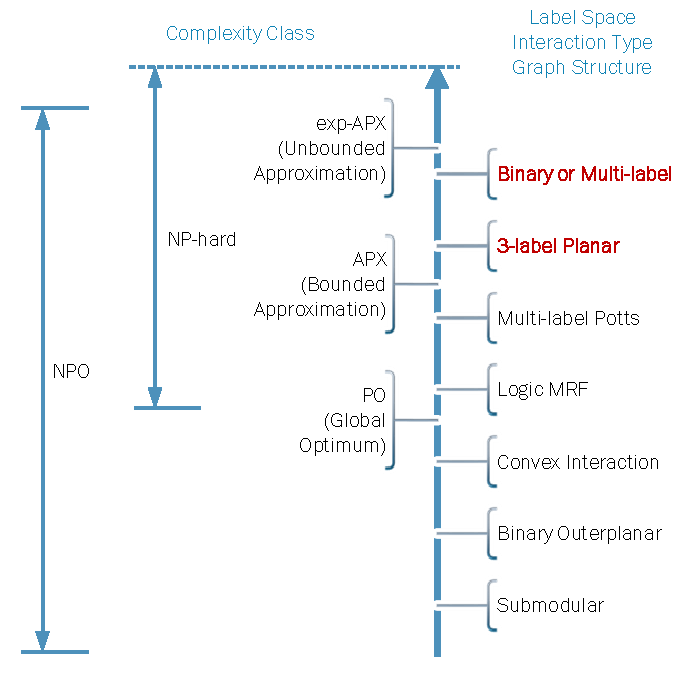
\includegraphics[width=0.6\linewidth]{figure/HardnessAxis.pdf}
\end{center}
    \caption{Discrete energy minimization problems aligned on a complexity axis. Red, boldface indicates new results proven in this paper. Note that problems are not ranked within a complexity class. Some problems discussed in this paper are removed for the simplicity of the figure.}
    % ** within a complexity class is not technically correct
\label{fig:hardnessaxis}
\end{figure}

% First contribution  QPBO and general case proof 
\textbf{Binary and multi-label case}  (Section~\ref{sec:gencase}). It is known that QPBO (2-label case) and the general energy minimization problem (multi-label case) are NP-hard~\cite{BorosHammer02}. They generalize such classical NP-hard optimization problems on graphs as vertex packing (maximum independent set) and the minimum and maximum cut problems~\cite{Karp-72}.
In this paper, we show a much stronger conclusion. \emph{We prove that QPBO as well as general energy minimization are complete (being the hardest problems) in the class exp-APX.} This implies that there can be no method in polynomial time to find an approximation within a constant factor of the optimal, {\red and in fact, the only possible factor in polynomial time is exponential in the input size}. % please delete if unsure
In practice, this means that a solution may be essentially arbitrarily bad.
Furthermore, all optimization problems in which merely finding a feasible solution is tractable are in exp-APX (see \Section{sec:prelim}) and thus QPBO, being exp-APX-complete, is amongst the hardest of them.
%In fact, any optimization problem, in which merely finding a feasible solution is tractable can be reduced to QPBO while preserving approximation ratio. It means that QPBO is as 


% 3 or more label planar graph contribution
\textbf{Planar three or more label case}  (Section~\ref{sec:plcase}). Planar graphs form the underlying graph structure for many computer vision and image processing tasks. It is known that efficient exact algorithms exist for some special cases of planar 2-label energy minimization, such as outerplanar~\cite{Schraudolph-10}.  In this paper, we show that for the case of three or more labels, planar energy minimization is exp-APX-complete, which means these problems are as hard as general energy minimization. The complexity of planar 2-label case remains an open question.

\textbf{Subclass problems}  (Section~\ref{sec:specialcases}). Special cases for some energy minimization algorithms relevant to computer vision are known to be tractable. However, detailed complexity analysis of these algorithms is patchy and spread across numerous papers.  In Section~\ref{sec:specialcases}, we classify the complexity of these subclass problems and illustrate some of their connections.  Such an analysis can help computer vision researchers become acquainted with existing complexity results relevant to energy minimization and can aid in selecting an appropriate model for an application or in designing new algorithms.






\subsection{Related Work}\label{sec:related}

% We focus on complexity, not applications.
% Most work is on harness (is it P or NP hard)
% Some work on complexity of approximation - where did this field come from
% - most detailed work is on other problems
% - or has weaker results
%

% We focus on theoretical and not empirical.  
Much of the work on complexity in computer vision has focused on experimental or empirical comparison of inference methods, including influential studies on choosing the best optimization techniques for specific classes of energy minimization problems~\cite{Szeliski08-PAMI,kappes2015comparative} and the PASCAL Probabilistic Inference Challenge, which focused on the more general context of inference in graphical models~\cite{PIC}. In contrast, our work focuses on theoretical computational complexity, rather than experimental analysis.

% Known results for NP-hardness not known for approximations
On the theoretical side, the NP-hardness of certain energy minimization problems is well studied. It has been shown that 2-label energy minimization is, in general, NP-hard, but it can be in PO if it is submodular~\cite{Kolmogorov02:regular-pami} or, \eg, outerplanar~\cite{Schraudolph-10}. For multi-label problems, the NP-hardness was proven by reduction from the NP-hard multi-way cut problem~\cite{boykov2001approximate}. These results, however, say nothing about the complexity of {\em approximating} the global optimum for the intractable cases. The complexity involving approximation has been studied for classical combinatorial problems, such as MAX-CUT and MAX-2SAT, which are known to be APX-complete~\cite{Papadimitriou-91}. QPBO generalizes such problems and is therefore APX-hard. This leaves a possibility that QPBO may be in APX, \ie, approximable within a constant factor.

% It is well-known that QPBO is NP-hard, since it generalizes such problems as maximum cut and maximum 2-satisfiability~\cite{Karp-72}. 
% These problems are also known to be APX-complete~\cite{Papadimitriou-91} (implies NP-hardness). Therefore, QPBO is APX-hard.


% Results for directed graphical models (one measure)
Energy minimization is often used to solve MAP inference for undirected graphical models. In contrast to scarce results for energy minimization and undirected graphical models, researchers have more extensively studied the computational complexity of approximating the MAP solution for {\em Bayesian networks}, also known as {\em directed graphical models}~\cite{kwisthout2015tree}. Abdelbar and Hedetniemi first proved the NP-hardness for approximating the MAP assignment of directed graphical models in the value of probability, \ie, finding $x$ such that
%\begin{align}\label{p-approx-ratio}
%\frac{p(x^*)}{p(x)} \leq r(n)
%\end{align}
$p(x^*)/ p(x) \leq r(n)$
with a constant or polynomial ratio $r(n) \geq 1$ is NP-hard, showing that this problem is poly-APX-hard~\cite{Abdelbar-98}. 
% ::: can we remove the following statement and footnote?  Is it really relevant to the related work here?
%This result holds even after restricting to binary variables and factors of order 3.\footnote{\citet[\parSym 6.1]{Abdelbar-98} count incoming edges of the network: for a factor $p(x_1 | x_2,x_3)$ there are two, but the total number of variables it couples is 3.} 
% ::: I am not sure the rest of this paragraph is needed either.
% ::: maybe add back in later.  Note that the approximation ratio for probabilities translates to an absolute approximation (an additive bound) for energies in a minimization problem.
% ::: added "in a minimization problem" is that true.
% ::: This is a good candidate for text to remove if we need space ->
% In addition, they showed that the following problems are also APX-hard:
% \begin{itemize}
% \item given the optimal solution, approximate the next optimal solution
% ** By reviewer: next optimal is really confusing
% \item given the optimal solution, approximate the optimal solution conditioned on changing the assignment of one variable
% \end{itemize}
The probability approximation ratio is closest to the energy ratio used in our work, but other approximation measures have also been studied.  \citeauthor{Kwisthout-11} showed the NP-hardness for approximating MAPs with the measure of additive value-, structure-, and rank-approximation~\cite{Kwisthout-11,Kwisthout-13,kwisthout2015tree}.
% ::: This next statement could easily be omitted, I think.
% ** Because NP-hardness does not apply to randomzied algorithms, there is no concise way of introducing expectation-approximation
He also investigated the hardness of expectation-approximation of MAP, and found that no randomized algorithm can expectation-approximate MAP in polynomial time with a bounded margin of error unless NP $\subseteq$ BPP, an assumption that is highly unlikely to be true~\cite{kwisthout2015tree}.

% Other approximation measures
%More recently, the hardness of MAP inference is studied in various approximation measures. Aside from ratio approximation, the NP-hardness has been shown for additive value-approximation of MAP \citet{Kwisthout-11}, structure-approximation of MAP \citet{Kwisthout-13}, rank-approximation of MAP \cite{kwisthout2015tree}. \citet{kwisthout2015tree} also investigated the hardness of expectation-approximation of MAP, and the finding is that no randomized algorithm can expectation-approximate MAP in polynomial time with bounded margin of error unless NP $\subseteq$ BPP, an assumption that is highly unlikely to be true.

% How is what we're doing different?
Unfortunately, the complexity results for directed models do not readily transfer to undirected models and vice versa. In directed and undirected models, the graph represents different conditional independence relations, thus the underlying family of probability distributions encoded by these two models is distinct, as detailed in Section~\ref{sec:BayesNet}. However, one can ask similar questions on the hardness of undirected models in terms of various approximation measures. In this work, we answer two questions, ``How hard is it to approximate the MAP inference in the ratio of energy (log probability) and the ratio of probability?'' The complexity of structure-, rank-, and expectation-approximation remain open questions for energy minimization.


% ::: removed text:  which results in a complexity claims that may sound contradictory (see~\autoref{fig-differences}). Roughly, NPO class by~\citet{Orponen90onapproximation} matches exp-APX class by~\citet{approx99}.

% \begin{table}[tb]
% \centering
% \setlength{\tabcolsep}{2pt}
% \begin{tabular}{|c|ccc|}
% \hline
% Source & Objective & Feasibility & Approximation Measure \\
% \hline
% \cite{Orponen90onapproximation} & non-negative & P &  cost-respecting\\
% \cite{approx99} & positive & NP &  performance ratio\\
% \hline
% \end{tabular}
% \caption{Two different sources of fundamental definitions\label{fig-differences}.}
% \end{table}
%::: this table seems a bit tacky.  I suggest removing it and then rewording the text to avoid needing it.  
% : updated the caption


% Paragraphs to be moved to the discussion after the corollary
% However, \eqref{p-approx-ratio} translates to an absolute energy approximation with a bound of $\log (r(n))$, \ie, logarithmic in $n$. We will show as a corollary from our result that it provides a stronger inapproximability for probabilities.

%The difference to our result is that approximation ration for MPE translates to additive approximation of energies (in order to translate a multiplicative factorization of a Belief Network to an additive one of the form~\eqref{eq:1}, the connection should be given by $p(x) = \exp(-E(x))$). 
%Additionally, their proof was given for a model involving four-tuple interactions (three-tuple in case of~\cite[\parSym 6.1]{Abdelbar-98}), and in this respect ours is a refinement. 
%We also imply a stronger hardness: while \cite{Abdelbar-98} shows it is NP-hard to approximate with a polynomial factor, we show it is NP-hard to approximate with a subexponential factor.
 % than poly-APX-hard.
%We will show as a corollary from our result that approximating in the value of probability is exp-APX-complete as well, which in particular implies the problem is poly-APX-hard.


% Maybe such basics clarification is better fit in the discussion section?

% NP-hardness has been shown for the MAP assignment of belief networks by~\citet{Cooper-90} and \citet{Shimony-94}. \citet{Abdelbar-98} has shown that approximating the MAP assignment is also NP-hard. However, there are substantial differences from our result.
% Belief networks have a probability density function $p(x)$ that factors according to a directed acyclic graph, \eg, as $p(x_1,x_2,x_3) = p(x_1 | x_2,x_3)p(x_2)p(x_3)$. %Using the relation $p(x) = \exp(-f(x))$, 
% %The negative logarithm of the pdf is then representable as a partially separable function of the form~\eqref{eq:1}. Maximization of the probability 
% For belief networks, finding the MAP assignment\footnote{Same as the most probable estimate (MPE).} in a Bayesian network is related to energy minimization~\eqref{eq:1} by letting $f(x) = -\log(p(x))$. The product is transformed into the sum and so, \eg, factor $p(x_1 | x_2,x_3)$ corresponds to term $f_{1,2,3}(x_1,x_2,x_3)$.
% %
% Note, factors of at most two variables, \eg, $p(x_1 | x_2)$, can form only a tree-structured model. % and therefore a Bayesian Network corresponding to a given energy may require higher order factors.
% %In the other direction, 
% Therefore, a Bayesian network corresponding to the pairwise energy~\eqref{eq:1} may require to use factors of order up to $|V|$. \revisit[this sentence is confusing] % in the Bayesian Network representation. 
% It is seen that while the general problems are convertible, fixed-parameter classes (such as order and graph restrictions) differ. In addition, approximation ratio for probabilities translates to an absolute approximation (an additive bound) for energies.


% \citet{Abdelbar-98} has shown that approximating the MAP assignment is also NP-hard. However, there are substantial differences from our result.


% are two neccessary conditions for the problem to be in PO. 


% It is well-known that QPBO is NP-hard, since it generalizes such problems as maximum cut and maximum 2-satisfiability~\cite{Karp-72}. 
% These problems are also known to be APX-complete~\cite{Papadimitriou-91} (implies NP-hardness). Therefore, QPBO is APX-hard.
% %::: this does not flow very well.  This next text is not really related work.  It is more about our work.  Maybe better to just say "In this paper, we prove the stronger claim that QPBO is complete in exp-APX."
% Completeness in exp-APX is stronger. 
%::: suggest moving the following text to the section on the proof.
% In particular, it shows that such problems as general traveling salesman problem (TSP) can be reduced to QPBO while preserving approximation ratio in a linear fashion.

\section{Definitions and Notation} \label{sec:prelim}

There are at least two different sets of definitions of what is considered an NP optimization problem~\cite{orponen1987approximation, ausiello1999complexity}. Here, we follow the notation of Ausiello et al~\cite{ausiello1999complexity} and restate the definitions needed for us to state and prove our theorems in Sections~\ref{sec:gencase} and \ref{sec:plcase} with our explanation of their relevance to our proofs.

\begin{definition}[Optimization Problem, \cite{ausiello1999complexity} Def. 1.16]An {\em optimization problem} $\P$ is characterized by a quadruple $(\I,\S,m,\text{goal})$ where
\begin{enumerate}
\item $\I$ is the set of instances of $\P$;
\item $\S$ is a function that associates to any input instance $x\in\I$ the set of {\em feasible solutions} of $x$;
\item and $m$ is the {\em measure} function, defined for pairs $(x,y)$ such that $x\in\I$ and $y\in\S(x)$. For every such pair $(x,y)$, $m(x,y)$ provides a  positive integer.
\item goal $\in$ \{MIN, MAX\}.

% \footnote{In practice, usually $m \in \mathcal{Q}$ the measure is usually defined in $\mathcal{Q}$ (rational numbers). However, it is possible to transform any such problem into an equivalent one where m is a positive integer. (cite)}
%satisfying our definition} which is the value of the feasible solution $y$. 

\end{enumerate}
\end{definition}
\noindent
Notice the assumption that the cost is positive, and, in particular, it cannot be zero.

%Analogous to NP and P for decision problems, we have NPO and PO for optimization problems:

\begin{definition}[Class NPO, \cite{ausiello1999complexity} Def 1.17] An optimization problem $\P = (\I,\S,m, \text{goal}$ $\in$ $\{\min , \max\} )$ belongs to the class of NP optimization (NPO) problems if the following hold:
\begin{enumerate}
\item The set of instances $\I$ is recognizable in polynomial time.
\item There exists a polynomial $q$ such that given an instance $x\in\I$, for any $y\in \S(x)$, $|y| < q(x)$ and, besides, for any $y$ such that $|y| < q(x)$, it is decidable in polynomial time whether $y\in\S(x)$.
\item The measure function $m$ is computable in polynomial time.
\end{enumerate}
\end{definition}

\begin{definition}[Class PO, \cite{ausiello1999complexity} Def 1.18] An optimization problem $\P$ belongs to the class of PO if it is in NPO and there exists a polynomial-time algorithm that, for any instance $x\in\I$, returns an optimal solution $y\in\S^*(x)$, together with its value $m^*(x)$.
\end{definition}

%For intractable problems, it may be acceptable to seek an approximate solution that is sufficiently close to optimal.

\begin{definition}[Approximation Algorithm, \cite{ausiello1999complexity} Def. 3.1]Given an optimization problem $\P = (\I,\S,m,\text{goal})$ an algorithm $\A$ is an {\em approximation algorithm} for $\P$ if, for any given instance $x\in\I$, it returns an {\em approximate solution}, that is a feasible solution $\A(x) \in \S(x)$.
\end{definition}

%
\begin{definition}[Performance Ratio, \cite{ausiello1999complexity}, Def. 3.6] \label{def:ratio} Given an optimization problem $\P$, for any instance $x$ of $\P$ and for any feasible solution $y\in\S(x)$, the {\em performance ratio}, {\em approximation ratio} or {\em approximation factor} of $y$ with respect to $x$ is defined as
\begin{align}
R(x,y) = \max\Big\{\frac{m(x,y)}{m^*(x)}, \frac{m^*(x)}{m(x,y)}\Big\},
\end{align}
where $m^*(x)$ is the measure of the optimal solution for the instance $x$.
\end{definition}
Since $m^*(x)$ is a positive integer, the performance ratio is well-defined. It is a rational number in $[1,\infty)$.
Notice that from this definition, it follows that if finding a feasible solution, \eg $y\in\S(x)$, is an NP-hard decision problem, then there exists no polynomial-time approximation algorithm for $\P$, irrespective of the kind of performance evaluation that one could possibly mean. 

\begin{definition}[$r(n)$-approximation, \cite{ausiello1999complexity}, Def. 8.1]Given an optimization problem $\P$ in NPO, an approximation algorithm $\A$ for $\P$, and a function $r\colon \Natural \to (1,\infty)$, we say that $\A$ is an {\em $r(n)$-approximate} algorithm for $\P$ if, for any instance $x$ of $\P$ such that $\S(x) \neq \emptyset$, the performance ratio of the feasible solution $\A(x)$ with respect to $x$ verifies the following inequality:
\begin{align}
R(x,\A(x)) \leq r(|x|).
\end{align}
\end{definition}

\begin{definition}[$F$-APX, \cite{ausiello1999complexity}, Def. 8.2]\label{def:F-APX} Given a class of functions $F$, $F$-APX is the class of all NPO problems $\P$ such that, for some function $r\in F$, there exists a polynomial-time $r(n)$-approximate algorithm for $\P$.
\end{definition}

The class of constant functions for $F$ yields the complexity class APX. Together with logarithmic, polynomial, and exponential functions applied in~\cref{def:F-APX}, the following {\em complexity axis} is established:
\begin{align}\notag                                           
\mbox{PO $\subseteq$ APX $\subseteq$ log-APX $\subseteq$ poly-APX $\subseteq$ exp-APX $\subseteq$ NPO}.
\end{align}

\noindent

Since the measure $m$ needs to be computable in polynomial time for NPO problems, the largest measure and thus the largest performance ratio is an exponential function. But exp-APX does not equal to NPO (assuming P $\neq$ NP) because NPO contains problems whose feasible solutions cannot be found in polynomial time.  For an energy minimization problem, any label assignment is a feasible solution, implying that all energy minimization problems are in exp-APX.

% While any energy minimization can be reduced to a Potts model~\cite{prusa2015hard},
% % ::: not actually in the next section
% there exists no reduction that preserves the approximation ratio because Potts model is in APX, an easier complexity class. Therefore proposing an algorithm employing such a reduction and quoting the 2-approximability of the Potts model would be an immediate mistake.

The standard approach for proofs in complexity theory is to perform a reduction from a known NP-complete problem.  Unfortunately, the most common polynomial-time reductions ignore the quality of the solution in the approximated case. For example, it is shown that any energy minimization problem can be reduced to a factor 2 approximable Potts model \cite{prusa2015hard}, however the reduction is not approximation preserving and is unable to show the hardness of general energy minimization in terms of approximation. Therefore, it is necessary to use an approximation preserving (AP) reduction to classify NPO problems that are not in PO, for which only the approximation algorithms are tractable.  AP-preserving reductions preserve the approximation ratio in a linear fashion, and thus preserve the membership in these complexity classes.  Formally,

\begin{definition}[AP-reduction, \cite{ausiello1999complexity} Def. 8.3]\label{def:AP-red}
Let $\P_1$ and $\P_2$ be two problems in NPO. $\P_1$ is said to be AP-{\em reducible} to $\P_2$, in symbols $\P_1 \leqAP \P_2$, if two functions $\pi$ and $\sigma$ and a positive constant $\alpha$ exist such that:
\begin{enumerate}
\item For any instance $x\in \I_1$ and for any rational $r > 1$, $\pi(x, r) \in \I_2$.
\item For any instance $x\in \I_1$ and for any rational $r > 1$, if $S_1(x) \neq \emptyset$ then $S_2(\pi(x,r)) \neq \emptyset$.
\item For any instance $x\in \I_1$, for any rational $r > 1$ and for any $y \in S_2(\pi(x,r))$, $\sigma(x, y, r) \in S_1(x)$.
\item $\pi$ and $\sigma$ are computable by algorithms whose running time is polynomial for any fixed rational $r$.
\item For any instance $x\in \I_1$, for any rational $r > 1$, and for any $y \in S_2(\pi(x,r))$,
\begin{align} \label{eq:AP-red}
R_2(\pi(x,r),y) \leq r \quad \text{implies} \\
R_1(x, \sigma(x, y, r)) \leq 1 + \alpha(r-1).
\end{align}
\end{enumerate}
\end{definition}

AP-reduction is the formal definition of the term `as hard as' used in this paper unless otherwise specified. It defines a partial order among optimization problems. With respect to this relationship, we can formally define the subclass containing the hardest problems in a complexity class:

\begin{definition}[$\C$-hard and $\C$-complete,  \cite{ausiello1999complexity} Def. 8.5]\label{def:complete} Given a class $\C$ of NPO problems, a problem $\P$ is $\C$-hard if, for any $\P' \in \C$, $\P' \leqAP \P$. A $\C$-hard problem is $\C$-complete if it belongs to $\C$.
\end{definition}

Intuitively, a complexity class $\C$ specifies the upper bound on the hardness of the problems within, $\C$-hard specifies the lower bound, and $\C$-complete exactly specifies the hardness.
\section{Inapproximability for the General Case} \label{sec:gencase}

% Start section with an overview:
% - explain the goal.  What is known, what you will show.
% - explain the process
%   - qpbo is a special case.
%   - prove that and then extend to general case.
In this section, we show that QPBO and general energy minimization are inapproximable by proving they are exp-APX-complete. As previously mentioned, it is already known that these problems are NP-hard \cite{BorosHammer02}, but it was previously unknown whether useful approximation guarantees were possible in the general case.  %We start our proof with the 2-label case QPBO, then we prove the more general case.
The formal statement of QPBO as an optimization problem is as follows:
\begin{problem}{\bf QPBO}
\begin{itemize}
\item[\sc instance:] A pseudo-Boolean function $f \colon \Bool^\V \to \Natural \colon$
\begin{align}
f(x) = \sum_{v\in\V} f_u(x_u) + \sum_{u,v\in\V} f_{uv}(x_u,x_v),
\end{align}
given by the collection of unary terms $f_u$ and pairwise terms $f_{uv}$.
\item[\sc solution:] Assignment of variables $x \in \Bool^\V$.
\item[\sc measure:] $\min f(x) > 0$.
\end{itemize}
\end{problem}

\begin{restatable}{theorem}{Tmain}\label{th:main}
%\begin{theorem} \label{th:main}
QPBO is exp-APX-complete.
%\end{theorem}
\end{restatable}
%\noindent
\begin{proofsketch} (Full proof in \cref{sec:formalproof}).
\begin{enumerate}
\item We observe that W3SAT-triv is known to be exp-APX-complete \cite{ausiello1999complexity}. W3SAT-triv is a 3-SAT problem with weights on the variables and an artificial, trivial solution.
\item Each 3-clause in the conjunctive normal form can be represented as a polynomial consisting of three binary variables. Together with representing the weights with the unary terms, we arrive at a 3-label energy minimization problem.
\item We use the method of~\cite{ishikawa2011transformation} to transform the 3-label problem into a 2-label one, with polynomially many additional variables, which is an instance of QPBO.
\item The transformation defines an injective forward mapping $\pi$ and then we define a surjective inverse mapping $\sigma$ to set up the two-way correspondence between W3SAT-triv and the transformed QPBO.
\item We prove that such mappings build an AP-reduction from W3SAT-triv to QPBO, \ie W3SAT-triv $\leqAP$ QPBO. This proves that QPBO is exp-APX-hard.
\item We observe that all energy minimization problems are in exp-APX and thereby concluding that QPBO is exp-APX-complete.
\end{enumerate}
\end{proofsketch}
% ::: If there is space, it would be good to flesh this proof sketch out a bit.  In particular, there i no intuition of what pi and sigma are in this brief sketch
% ** sigma cannot be explained before formally showing W3SAT-triv

This inapproximability result can be generalized to more than two labels.
\begin{restatable}{corollary}{Cgen}\label{C:gen}
$k$-label energy minimization is exp-APX-complete for $k \geq 2$.
\end{restatable}
%
%\noindent
%\textbf{Proof sketch} 
\begin{proofsketch}
(Full proof in \cref{sec:formalproof}). This theorem is proved by showing QPBO $ \leqAP$ $k$-label energy minimization for $k \geq 2$.
\end{proofsketch}
%We show in \cref{C:prob-approx} the inapproximability in energy (log probability) transfer to probability in Equation~\cref{p-approx-ratio} as well.

 Our result also implies inapproximablity of MAP in the measure of probability (as studied for directed networks by~\citet{Kwisthout-13}). For undirected models the probability is given by the associated Gibbs distribution: $p(x) = \exp(-E(x))$.
 \begin{restatable}{corollary}{CprobApprox}\label{C:prob-approx}
 It is NP-hard to find a solution $x^*$ to MAP such that $p(x^*)/p(x) < \exp(r(n))$ for any given polynomial $r$.
 %\end{corollary}
 \end{restatable}
 \begin{proofsketch}
 (Full proof in \cref{sec:formalproof}). Note that a ratio $r(n)$ in the energy leads to $\Theta(\exp(r(n)))$ for the ratio in probability.
 \end{proofsketch}

Taken together, this theorem and its corollaries form a very strong inapproximability result for general energy minimization. They imply not only NP-hardness, but also that there is no algorithm that can approximate general energy minimization with two or more labels with an approximation ratio better than {\red some exponential function in the input size}. In other words, any approximation algorithm of the general energy minimization problem can perform arbitrarily badly, and it would be pointless to try to prove a bound on the approximation ratio for existing approximation algorithms for the general case.  While this conclusion is disappointing, these results serve as a clarification of grounds and guidance for model selection and algorithm design. Instead of counting on an oracle that solves the energy minimization problem, researchers should put efforts into selecting the proper formulation, trading off expressiveness for tractability. % For example, since QPBO is harder than MAXCUT it might be preferable to use MAXCUT as a model in a specific application or as a sub-problem solver in a general optimization algorithm.

% Note all the above discussion (collorary 
%In sum, these results amount to that any approximation algorithm of the general energy minimization problem can perform arbitrarily bad and it might be pointless to try to prove the approximation bound of existing approximation algorithms in the general case. 
% \par
% These inapproximability results should be understood not as disappointing facts (as they were in fact expected) but as a clarification of grounds and guidance for model selection and algorithms design. For example, since QPBO is harder than MAXCUT it might be preferable to use MAXCUT as a model in a specific application or as a subproblem solver in a general optimization algorithm. While any energy minimization can be reduced to a Potts model (see next section), there exist no reduction that preserves approximation ratio because Potts model is in APX, an easier complexity class. Therefore proposing an algorithm employing such a reduction and quoting the 2-approximability of Potts model would be an immediate mistake.
\section{Inapproximability for the Planar Case} \label{sec:plcase}

\begin{figure}[b]
\begin{center}
   
\includegraphics[width=1\linewidth]{figure/PlanarComplexity.pdf}
\end{center}
   \caption{Complexity for planar energy minimization problems. The ``general case'' implies no restrictions on the pairwise interaction type.  This paper shows that the third category of problems is not efficiently approximable.}
\label{fig:planarcomp}
\end{figure}

Efficient algorithms for energy minimization have been found for special cases of 2-label planar graphs.  Examples include planar 2-label problems without unary terms and outerplanar 2-label problems (i.e., the graph structure remains planar after connecting to a common node)~\cite{Schraudolph-10}. 
% ::: safe to omit - most everyone knows what a planar graph is
% {\em Planar graphs} are graphs that can be drawn on the plane in such a way that its edges intersect only at their endpoints.
Grid structures over image pixels naturally give rise to planar graphs in computer vision.  Given their frequency of use in this domain, it is natural to consider the complexity of more general cases involving planar graphs. Figure~\ref{fig:planarcomp} visualizes the current state of knowledge  of the complexity of energy minimization problems on planar graphs.  In this section, we prove that for the case of planar graphs with three or more labels, energy minimization is exp-APX-complete. This result is important because it significantly reduces the space of potentially efficient algorithms on planar graphs.  The approximibility of the general case for planar 2-label problems an open question.

\begin{restatable}{theorem}{Tplanar}\label{th:planar}
Planar 3-label energy minimization is exp-APX-complete.
\end{restatable}
%\noindent
%\textbf{Proof sketch} 
\begin{proofsketch}
(Full proof in \cref{sec:formalproof}).
\begin{enumerate}
    \item We construct elementary gadgets to reduce any 3-label energy minimization problem to a planar one with polynomially many auxiliary nodes.
    \item The above reduction defines an injective forward mapping and we define a surjective inverse mapping $\sigma$ to set up the two-way correspondence between the original problem and the reduced planar one.
    \item We prove that such mappings build an AP-reduction, \ie, 3-label energy minimization $\leqAP$ planar 3-label energy minimization.
    \item Since 3-label energy minimization is exp-APX-complete (\cref{C:gen}) and all energy minimization problems are in exp-APX, we thereby conclude that planar 3-label energy minimization is exp-APX-complete.
\end{enumerate}
\end{proofsketch}
\begin{restatable}{corollary}{Cplanark}\label{C:planark}
Planar $k$-label energy minimization is exp-APX-complete, for $k \geq 3$.
\end{restatable}
%\textbf{Proof sketch} 
\begin{proofsketch}
(Full proof in \cref{sec:formalproof}).
This theorem is proved by showing planar 3-label energy minimization $ \leqAP$ planar $k$-label energy minimization, for $k \geq 3$. 
\end{proofsketch}
These theorems show that the restricted case of planar graphs with 3 or more labels is as hard as general case for energy minimization problems with the same inapproximable implications discussed in Section~\ref{sec:gencase}.

The most novel and useful aspect of the proof of Theorem~\ref{th:planar} is the planar reduction in Step 1. The reduction creates an equivalent planar representation to any non-planar 3-label graph.  That is, the graphs share the same optimal value.  The reduction applies elementary constructions or ``gadgets'' to uncross two intersecting edges. This process is repeated until all intersecting edges are uncrossed. Similar elementary constructions were used to study the complexity of the linear programming formulation of energy minimization problems~\cite{prusa2015universality,prusa2015hard}.
Our novel gadgets have three key properties {\em at the same time}: 1) they are able to uncross intersecting edges, 2) they work on non-relaxed problems, \ie, all indicator variables (or pseudomarginals to be formal) are integral; and 3) they can be applied repeatedly to build an AP-reduction.


%This reduction is similar to the method used in~\cite{prusa2015universality}, except that our approach applies to the non-relaxed case, whereas the method in~\cite{prusa2015universality} applies only to the relaxed case.  

%
%On the other hand, it does not make sense to reduce TSP to QPBO, as   
%\begin{figure}
%\RawFloats
%\centering
%\begin{minipage}{.5\textwidth}
  %\centering
   %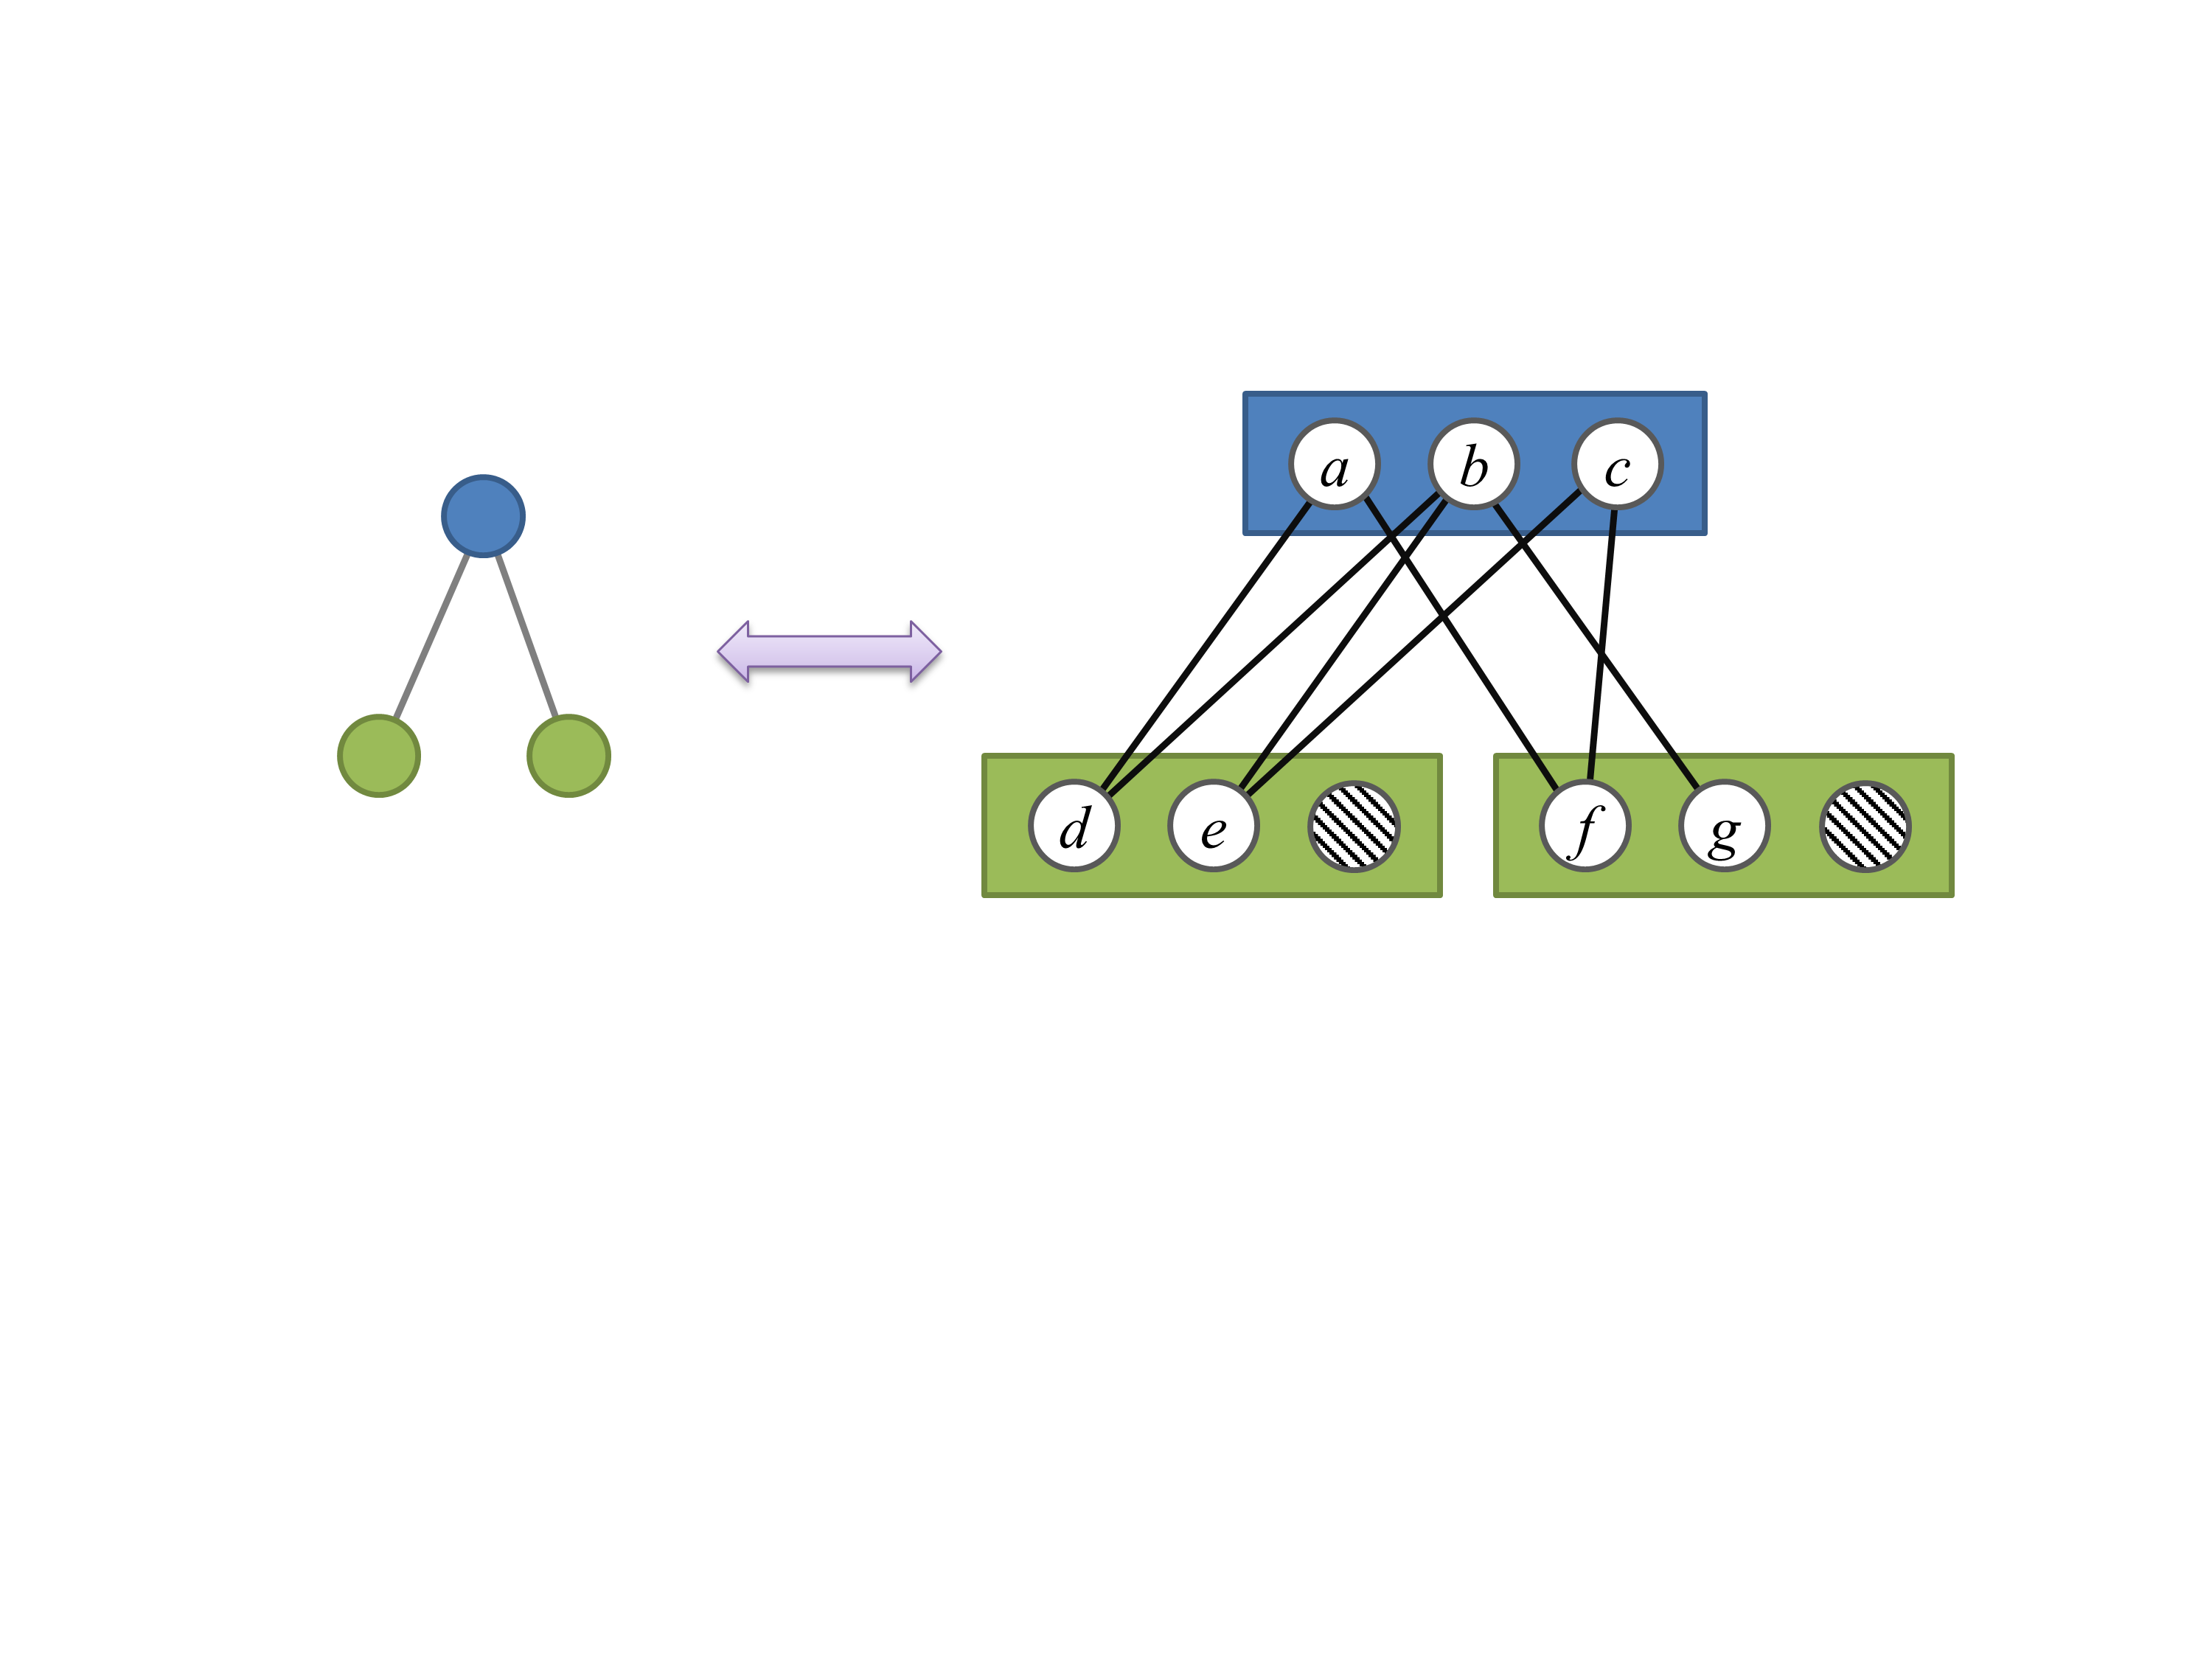
\includegraphics[trim={0 5cm 0 0}, clip, width=1.15\linewidth]{figure/Planar/Slide1.PNG}
   %\caption{{\sc Split}} \label{fig:split}
%\end{minipage}%
%\begin{minipage}{.5\textwidth}
  %\centering
   %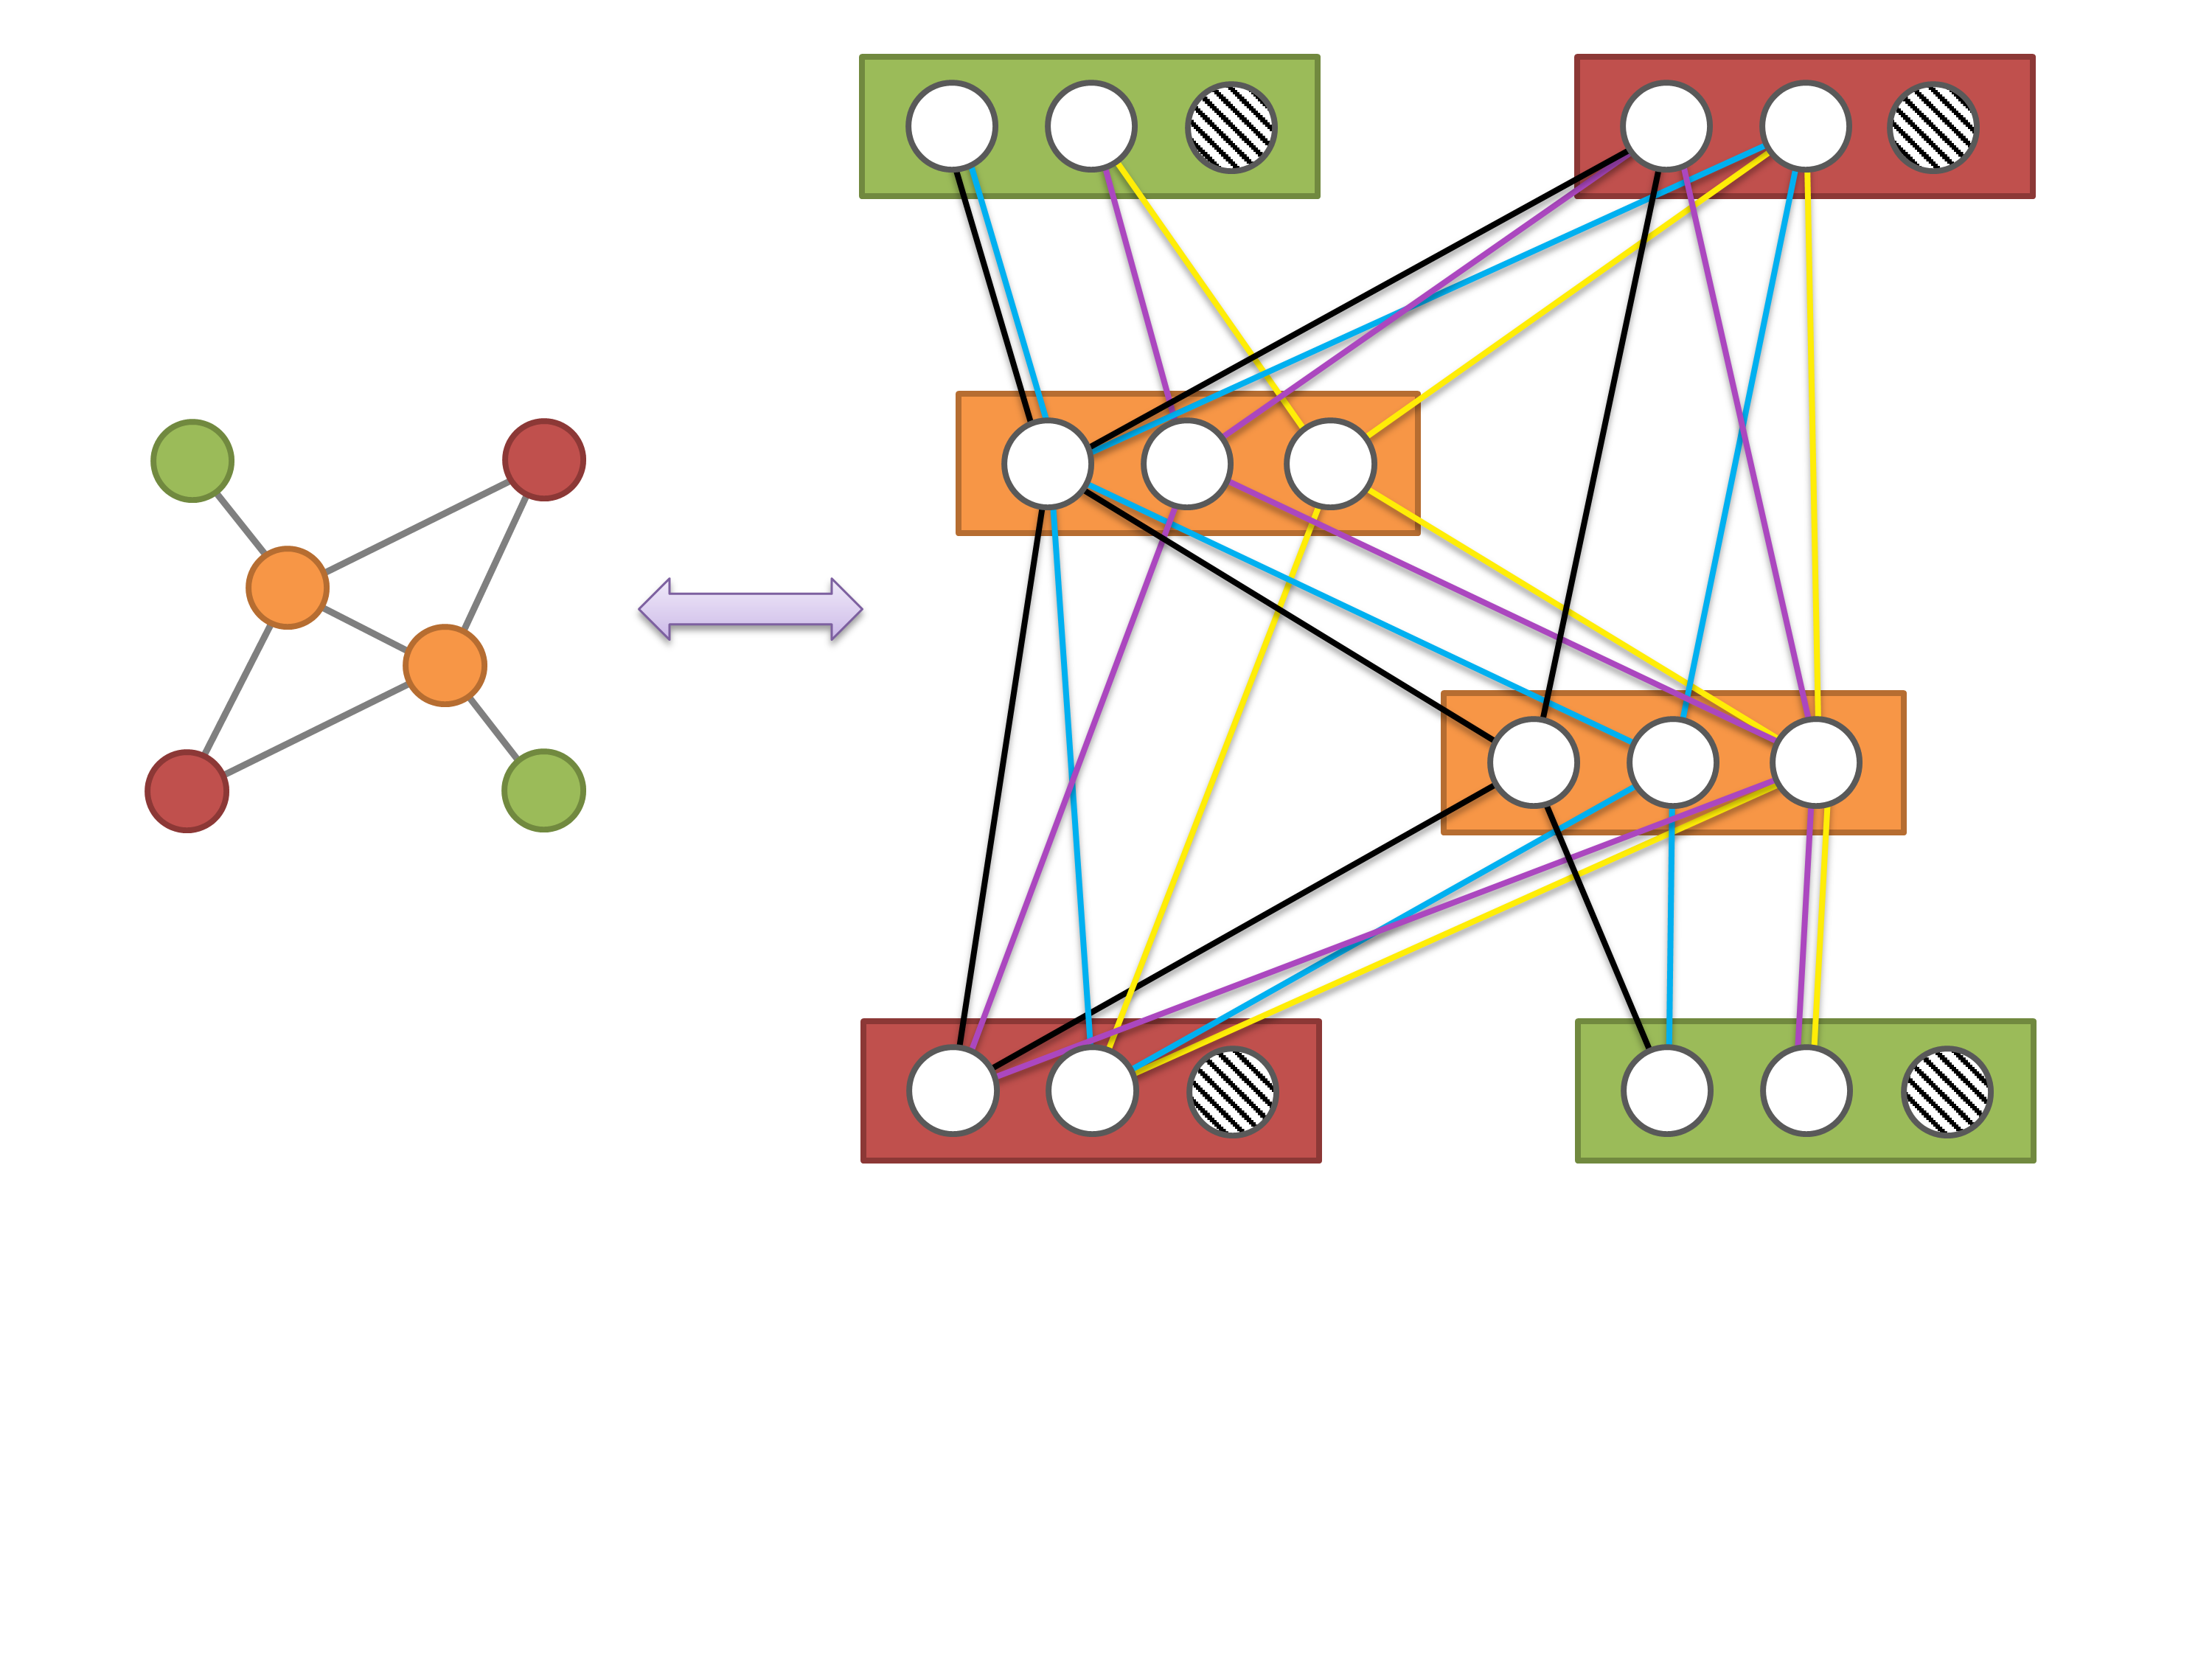
\includegraphics[trim={0 5cm 0 0}, clip, width=1.15\linewidth]{figure/Planar/Slide2.PNG}
   %\caption{{\sc UncrossCopy} } \label{fig:uncrosscopy}
%\end{minipage}
%\end{figure}
\begin{figure}
\centering
\begin{tabular}{cc}
\begin{tabular}{c}%
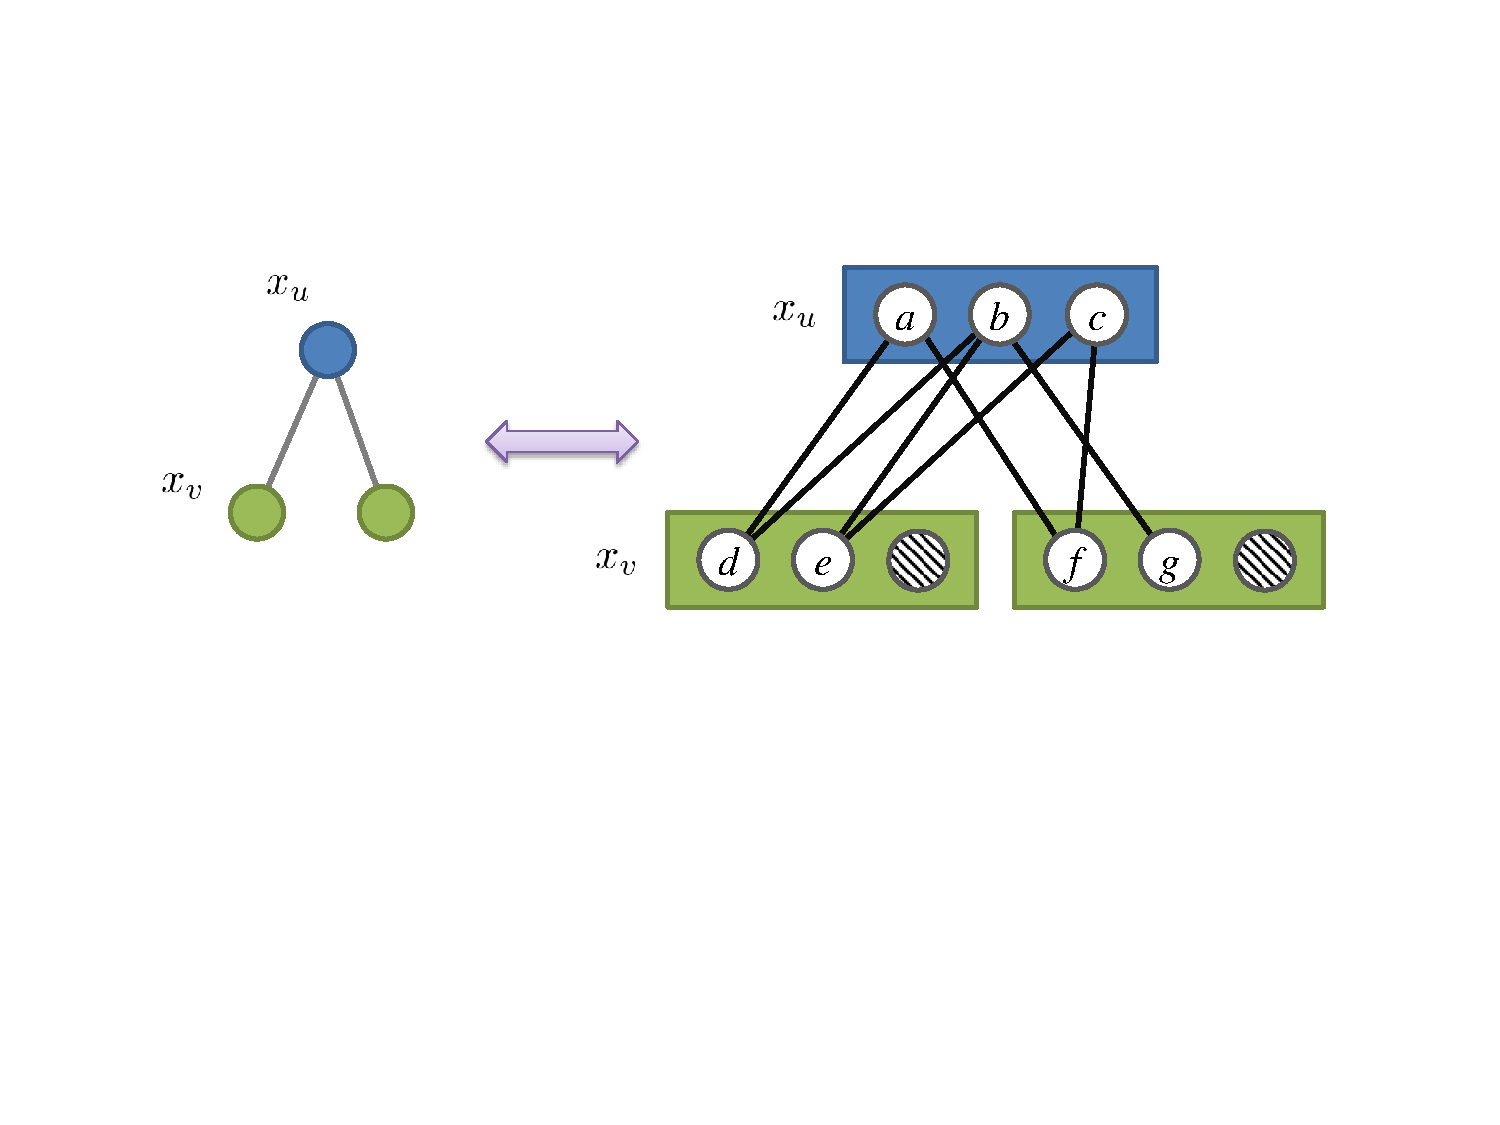
\includegraphics[width=0.39\linewidth]{figure/Planar/Planar-1-crop.pdf}
\end{tabular}&\ \ \ \ \ \ 
\begin{tabular}{c}%
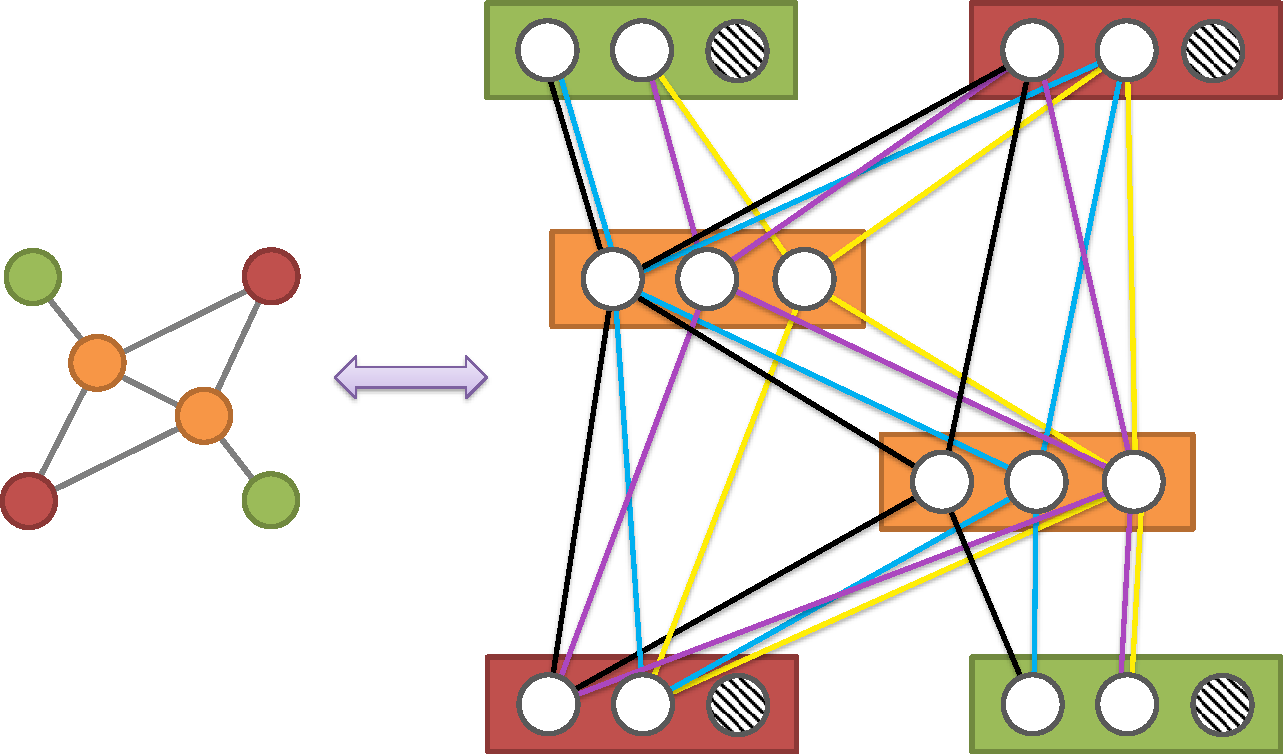
\includegraphics[width=0.39\linewidth]{figure/Planar/Planar-2-crop.pdf}
\end{tabular}\\
{\sc Split} & {\sc UncrossCopy}
\end{tabular}
\caption{Gadgets to represent a 3-label variable as two 2-label variables ({\sc Split}) and to copy the values of two diagonal pairs of 2-label variables without edge crossing ({\sc UncrossCopy}).\label{fig:split}}
\end{figure}

% 
The two gadgets used in our reduction are illustrated in Figure~\ref{fig:split}. A 3-label node can be encoded as a collection of 3 indicator variables with a one-hot constraint. In the figure, a solid colored circle denotes a 3-label node, and a solid colored rectangle denotes the equivalent node expressed with indicator variables (white circles).  For example, in Figure~\ref{fig:split}, $a=1$ corresponds to the blue node taking the first label value. The pairwise potentials (edges on the left part of the figures) can be viewed as edge costs between the indicator variables (black lines on the right), \eg, $f_{uv}(3, 2)$ is placed onto the edge between indicator $c$ and $e$ and is counted into the overall measure if and only if $c = e = 1$. In our gadgets, drawn edges represent zero cost while omitted edges represent positive infinity\footnote{A very large number will also serve the same purpose, \eg, take the sum of the absolute value of all energy terms and add 1. Therefore, we are not expanding the set of allowed energy terms to include $\infty$.}.  While the set of feasible solutions remains the same, the gadget encourages certain labeling relationships, which, if not satisfied, cause the overall measure to be infinity. Therefore, the encouraged relationships must be satisfied by any optimal solution. The two gadgets serves different purposes:

\textsc{Split} A 3-label node (blue) is split into two 2-label nodes (green). The shaded circle represents a label with a positive infinite unary cost and thus creates a simulated 2-label node. The encouraged relationships are
\begin{itemize}
    \item $a = 1 \leftrightarrow d = 1 \text{ and } f = 1$.
    \item $b = 1 \leftrightarrow g = 1$.
    \item $c = 1 \leftrightarrow e = 1 \text{ and } f = 1$.
\end{itemize}
Thus $(d,f)$ encodes $a$, $(d,g)$ and $(e,g)$ both encode $b$ and $(e,f)$ encodes $c$.

\textsc{UncrossCopy} The values of two 2-label nodes are encouraged to be the same as their diagonal counterparts respectively (red to red, green to green) without crossing with each other. The orange nodes are intermediate nodes that pass on the values. All types of lines represent the same edge cost, which is 0. The color differences visualize the verification for each of the 4 possible states of two 2-label nodes.  For example, the cyan lines verify the case where the top-left (green) node takes the values (1, 0) and the top-right (red) node takes the value (0, 1).  It is clear that the encouraged solution is for the bottom-left (red) node to take the value (0, 1), and the bottom-right (green) node to take the value (1, 0).

\begin{figure}
\begin{center}
   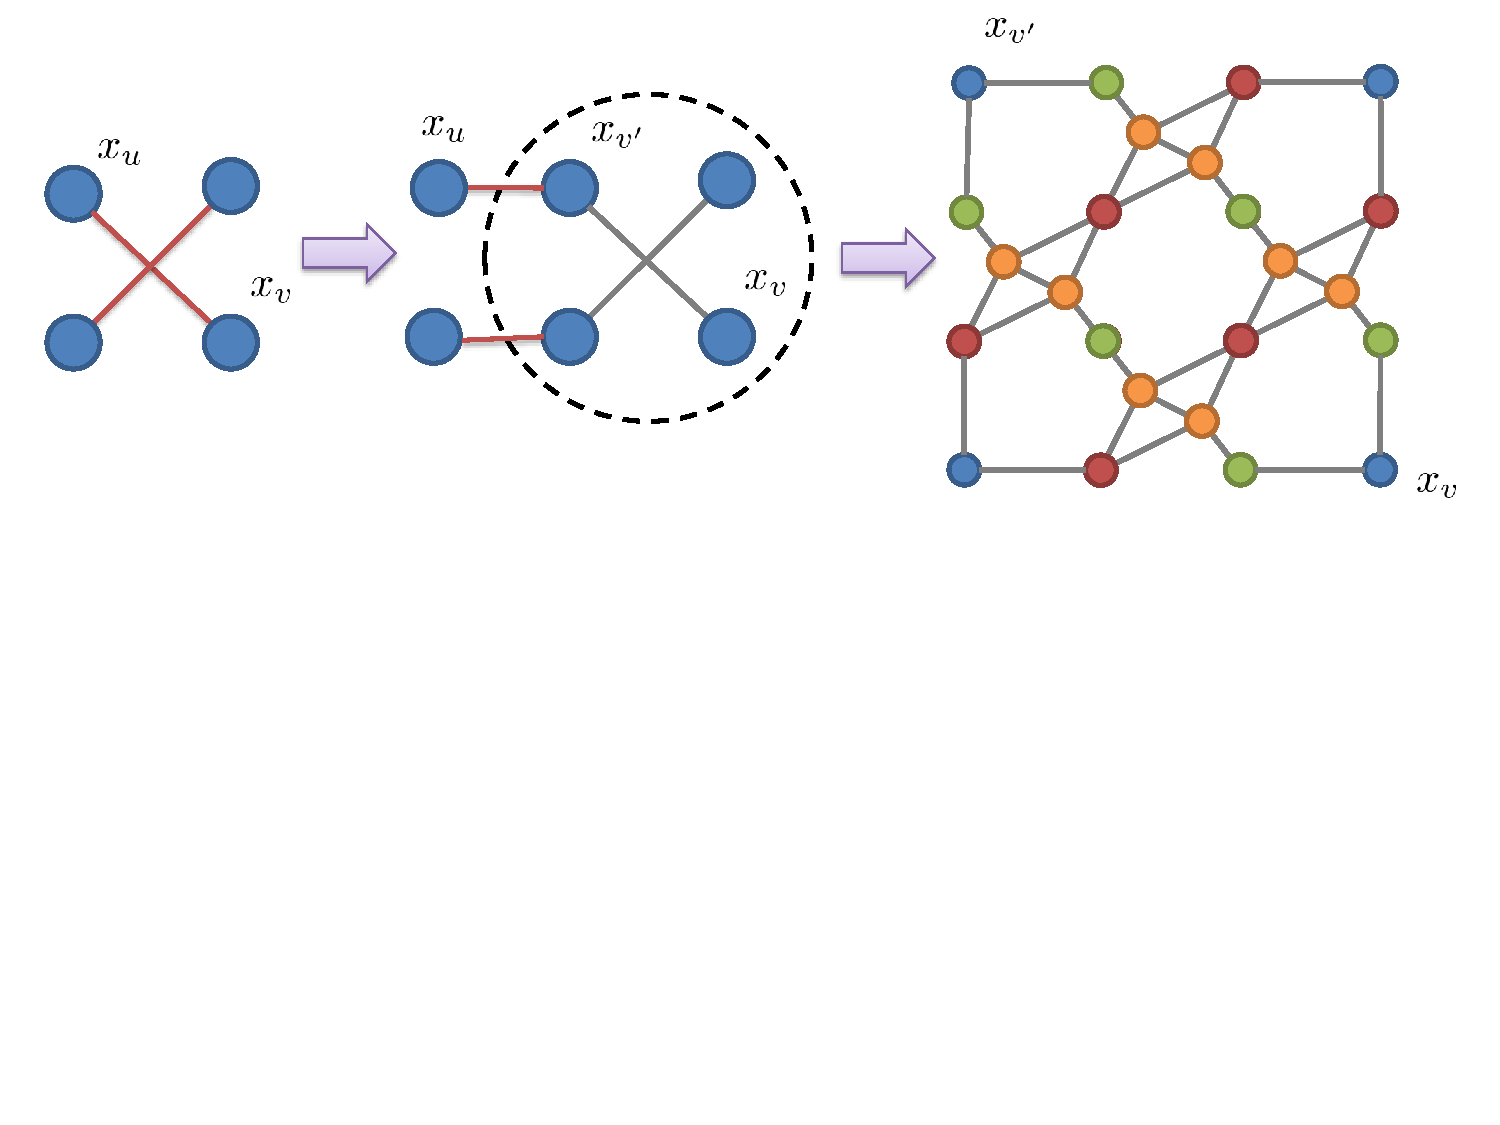
\includegraphics[trim={0 10.5cm 0 0}, clip, width=0.7\linewidth]{figure/Planar/Planar-3.pdf}
\end{center}
\caption{Planar reduction for 3-label problems} \label{fig:planarreduct}
\end{figure}

These two gadgets can be used to uncross the intersecting edges of two pairs of 3-label nodes (Figure~\ref{fig:planarreduct}, left).  For a crossing edge ($x_u$, $x_v$), first a new 3-label node $x_v'$ is introduced preserving the same arbitrary interaction (red line) as before (Figure~\ref{fig:planarreduct}, middle). Then, the crossing nodes (shown within the dotted circle) are uncrossed by applying {\sc Split} and {\sc UncrossCopy} four times (Figure~\ref{fig:planarreduct}, right).
Without loss of generality, we can assume that no more than two edges intersect at a common point except at their endpoints.  This process can be applied repeatedly at each edge crossing until there are no edge crossings left in the graph~\cite{prusa2015universality}.

% \section{Our Results}\label{sec:results}

%This section presents our contribution to the study of complexity for energy minimization problems.
\subsection{Definitions}
The formal statement of the announced contribution requires the following notions: what is understood as a NP optimization problem in general and QPBO problem in particular and how the complexity classes are defined with the help of an approximation preserving reduction. The most important parts of this structure are as follows.

%\par Unfortunately, there are slightly different versions of what to be considered as optimization problem \cite{orponen1987approximation, ausiello1999complexity}. We found \cite{ausiello1999complexity} to be the most consistent reference. % and we specialize these definitions here to the case of minimization problems for clarity.
Unfortunately, different authors adopt different definitions of NP optimization problems and approximability, which results in a complexity claims that may sound contradictory, see~\autoref{fig-differences}. Roughly, NPO class by~\citet{Orponen90onapproximation} matches exp-APX class by~\citet{approx99}.
\begin{table}[tb]
\centering
\setlength{\tabcolsep}{2pt}
\begin{tabular}{|c|ccc|}
\hline
Source & Objective & Feasibility & Approximation Measure \\
\hline
\cite{Orponen90onapproximation} & non-negative & P &  cost-respecting\\
\cite{approx99} & positive & NP &  approx. ratio\\
\hline
\end{tabular}
\caption{Some differences in definitions\label{fig-differences} of the class of NP optimization problems in the literature.}
\end{table}
%\par
Since one may arrive at a different claims, depending on these definitions, it is essential to state them precisely here. We follow~\citet{approx99} as the most consistent reference.
%
\begin{definition}[\cite{ausiello1999complexity}, Def. 1.16]A {\em minimization problem} $\P$ is characterized by a triplet $(\I,\S,m)$ where
\begin{enumerate}
\item $\I$ is the set of instances of $\P$;
\item $\S$ is a function that associates to any input instance $x\in\I$ the set of {\em feasible solutions} of $x$;
\item $m$ is the {\em measure} (or {\em cost} in context of minimization) function, defined for pairs $(x,y)$ such that $x\in\I$ and $y\in\S(x)$. For every such pair $(x,y)$, $m(x,y)$ provides a {\bf positive integer}\footnote{In practice, the measure is usually defined in $\mathcal{Q}$. It is however possible to transform any such problem into an equivalent one satisfying our definition} which is the value of the feasible solution $y$. 
\end{enumerate}
\end{definition}
Notice, the important part of this definition, besides notation convention, is the assumption that the cost is positive, in particular it cannot be zero.
Analogous to NP and P for decision problems, we have NPO and PO for optimization problems.
%
\begin{definition}[\cite{ausiello1999complexity}, Def 1.17] A minimization problem $\P = (\I,\S,m)$ belongs to the class of NP minimization (NPO) problems if the following holds:
\begin{enumerate}
\item the set of instances $I$ is recognizable in polynomial time.
\item there exists a polynomial $q$ such that given an instance $x\in\I$, for any $y\in \S(x)$, $|y| < q(x)$ and, besides, for any $y$ such that $|y| < q(x)$, it is decidable in polynomial time whether $y\in\S(x)$.
\item the measure function $m$ is computable in polynomial time.
\end{enumerate}
\end{definition}

%
\begin{definition}[\cite{ausiello1999complexity}, Def. 3.6]Given a minimization problem $\P$, for any instance $x$ of $\P$ and for any feasible solution $y\in\S(x)$, the {\em performance ratio} of $y$ with respect to $x$ is defined as
\begin{align}
R(x,y) = \frac{m(x,y)}{m^*(x)},
\end{align}
where $m^*(x)$ is the cost of the optimal solution.
\end{definition}
Now, since $m^*(x)$ is a positive integer, the performance ratio is well-defined, it is a rational number in $[1,\infty)$.
Notice, already from this definition follows that if finding a feasible solution, \eg $y\in\S(x)$, is an NP-hard decision problem, then there exist no {\em polynomial-time} approximation algorithm for $\P$. And this is irrespective of the kind of performance evaluation that one could possibly mean. The energy minimization~\eqref{eq:1} is easier than that - finding a feasible solution does not present a problem.
\begin{definition}[\cite{ausiello1999complexity}, Def. 8.1]Given an optimization problem $\P$ in NPO, an approximation algorithm $\A$ for $\P$, and a function $r\colon \Natural \to (1,\infty)$, we say that $\A$ is an {\em $r(n)$-approximate} algorithm for $\P$ if, for any instance $x$ of $\P$ such that $\S(x) \neq \emptyset$, the performance ratio of the feasible solution $\A(x)$ with respect to $x$ verifies the following inequality:
\begin{align}
R(x,\A(x)) \leq r(|x|).
\end{align}
\end{definition}
\begin{definition}[\cite{ausiello1999complexity}, Def. 8.2]\label{def:F-APX} Given a class of functions $F$, $F$-APX is the class of all NPO problems $\P$ such that, for some function $r\in F$, there exists a polynomial-time $r(n)$-approximate algorithm for $\P$.
\end{definition}

For $F$ being the class of constant functions, we get the complexity class APX. Together with logarithmic, polynomials and exponent functions used in~\cref{def:F-APX}, the following classification ruler is established:
\begin{align}\notag                                                                                                                                                          
\mbox{PO $\subseteq$ APX $\subseteq$ log-APX $\subseteq$ poly-APX $\subseteq$ exp-APX $\subseteq$ NPO}.
\end{align}


\subsection{Results}
%The following formally introduces what is understood as QPBO problem:
As we seen above an optimization problem is specified by a set of its instances, set of its solutions and the objective. We have
\begin{problem}{\bf QPBO}
\begin{itemize}
\item[\sc instance:] A pseudo-Boolean function $f \colon \Bool^\V \to \Natural \colon$
\begin{align}
f(x) = \sum_{v\in\V} f_u(x_u) + \sum_{u,v\in\V} f_{uv}(x_u,x_v),
\end{align}
given by the collection of unary terms $f_u$ and pairwise terms $f_{uv}$.
\item[\sc solution:] Assignment of variables $x \in \Bool^\V$.
\item[\sc measure:] $f(x) > 0$.
\end{itemize}
\end{problem}

\begin{restatable}{theorem}{Tmain}\label{th:main}
%\begin{theorem} \label{th:main}
QPBO is exp-APX-complete.
%\end{theorem}
\end{restatable}
\par
%\vskip\0.5\baselineskip
In the proof we construct a reduction from the weighted 3-satisfiability problem (W3SAT) using reduction by Ishikawa~\cite{ishikawa2011transformation} and show that the reduction preserves approximation ratio. We then use the known result that W3SAT can be used to solve any optimization problem encoded by a Turing machine and thus is complete in the class exp-APX.
Next, we show that restricting to planar 3-label energy minimization is also as hard:
%In addition, we construct a reduction that converts any 3-label energy minimization problems into a planar one. 
%This reduction is an approximation preserving (AP) one (will be defined and explained in \cref{sec:appendix}), thus showing that planar 3-label energy minimization is as hard as any arbitrary 3-label energy minimization. Therefore, we have the following theorem:
\begin{restatable}{theorem}{Tplanar} \label{th:planar}
Planar 3-label energy minimization is exp-APX-complete.
\end{restatable}
This result uses reduction gadgets inspired by a similar construction for reduction of LP-relaxations~\cite{prusa2015hard,Prusa-Werner-15-Universality}. Similar to these works we show how some edges may be uncrossed using auxiliary variables. Differently from them, the gadgets reduce integer solutions and not relaxed once (indeed their gadgets are infeasible for the discrete problem).
\par
The implications of the above theorems are further explained by the following corollaries. % (assuming P $\neq$ NP)

%\begin{corollary}
%QPBO is NP-hard.
%\end{corollary}

%\begin{corollary}
\begin{restatable}{corollary}{CexpApprox}\label{C:exp-approx}
There is no algorithm that can approximate QPBO  or planar 3-label energy minimization with an approximation ratio better than some exponential functions in the input size.
\end{restatable}
%\end{corollary}

%\begin{corollary}
This next corollary relates to the existing results for Bayesian networks.
\begin{restatable}{corollary}{CprobApprox}\label{C:prob-approx}
Probability ratio approximation is poly-APX-hard: it is NP-hard to approximate MAP in the value of probability~\eqref{p-approx-ratio} with any polynomial ratio $r(n)$.
%\end{corollary}
\end{restatable}

Naturally, the above results hold for the general form in (\ref{eq:1}) with arbitrary label space $\mathcal{L}$, as it contains all instances of QPBO.
There is one other corollary for the general problem:

\begin{restatable}{corollary}{ClabelApprox}\label{C:label-approx}
There is no algorithm that can approximate $k$-label energy minimization with an approximation ratio better or equal than some polynomials in $k$.
\end{restatable}
%\vskip0.5\baselineskip
\par
%In sum, these results amount to that any approximation algorithm of the general discrete energy minimization problem can perform arbitrarily bad and it might be pointless to try to prove the approximation bound of existing approximation algorithms in the general case. 
\par
These inapproximability results should be understood not as disappointing facts (as they were in fact expected) but as a clarification of grounds and guidance for model selection and algorithms design. For example, since QPBO is harder than MAXCUT it might be preferable to use MAXCUT as a model in a specific application or as a subproblem solver in a general optimization algorithm. While any energy minimization can be reduced to a Potts model (see next section), there exist no reduction that preserves approximation ratio because Potts model is in APX, an easier complexity class. Therefore proposing an algorithm employing such a reduction and quoting the 2-approximability of Potts model would be an immediate mistake.
%
%On the other hand, it does not make sense to reduce TSP to QPBO, as   
%
%These results are indeed disappointing, but as we have discussed, many of its subclass problems are relatively tractable. 
%We should not count on an oracle that solves the energy minimization problem. Instead, we should put efforts into selecting the proper formulation, trading off expressiveness for tractability.
%
%Implications of \cref{th:main} apply here as well. 
%The reduction itself might be useful if 3-label planar energy minimization is tractable. Yet, we present the reduction here as an inspiration for algorithmic design and proofs.



\section{Complexity of Subclass Problems} \label{sec:specialcases}

% The hardness of a discrete energy minimization problem depends on the graph structure, the interaction type and the label space. 

In this section, we classify some of the special cases of energy minimization according to our complexity axis (Figure~\ref{fig:hardnessaxis}). This classification can be viewed as a reinterpretation of existing results from the literature into a unified framework.

\subsection{Class PO (Global Optimum)}
% ::: would be worthwhile to add a sentence like this:
% ** I think it's fine without it
% The first set of algorithms we consider are in class PO, and thus a global optimum may be found in polynomial time with respect to the input.

Polynomial time solvability may be achieved by considering two principal restrictions: those restricting the {\em structure} of the problem, \ie, the graph $G$, and those restricting the type of allowed interactions, \ie, functions $f_{uv}$.
%\begin{itemize}
%    \item Structure restrictions: tree, bounded tree width, outer planar.
%    \item Interaction restrictions: characterization, bsiubmodular, submodular, convex, mincut.
%    \item Unary constraints and mixed pairwise-unary constraints.
%\end{itemize}

\textbf{Structure Restrictions.} When $G$ is a chain, energy minimization
% ~\eqref{eq:1}
reduces to finding a shortest path in the trellis graph, which can be solved using a classical dynamic programming method known, \eg, as the Viterbi algorithm~\cite{forney1973viterbi}.
%the Viterbi algorithm~\cite{forney1973viterbi}.
%::: get a better cite for viterbi.  do not cite wikipedia (ever).  you are not in 4th grade.
%:::old text: a classical dynamic programming method known, \eg, as Viterbi algorithm~\cite{wikipedia}.
%## What one can learn from wikipedia is that Viterbi was only onle of the gentelmen who have proposed such algorithms in different context
%When $G$ is a tree, the same DP principle applies: given a fixed state of a node the problem decouples into independent minimizations.
The same dynamic programming (DP) principle applies to graphs of bounded tree-width.  Fixing all variables in a separator set decouples the problem into independent optimization problems. For treewidth 1, the separators are just individual vertices and the problem is solved by a variant of DP~\cite{Pearl-88,SchlesingerHlavac2002}.
For higher treewidth, the respective optimization procedure is known as junction tree decomposition~\cite{Lauritzen96}. A loop is a simple example of a treewidth 2 problem. However, for a treewidth $k$, the time complexity is exponential in $k$~\cite{Lauritzen96}.
Finally, when $G$ is an outer-planar graph, the problem can be solved by the method of~\cite{Schraudolph-10}, which reduces it to a planar Ising model, for which efficient algorithms exist~\cite{Shih-90}.


\textbf{Interaction Restrictions.}
%Binary image segmentation with attractive interactions reduces to a minimum cut problem~\cite{Greig89}.
% Binary energy minimization with attractive interactions reduces to minimum cut problem~\cite{Greig89}. The set of problems solvable in this way is closely related to submodularity.
Submodularity is a restriction closely related to problems solvable by minimum cut. A quadratic pseudo-Boolean function $f$ is {\em submodular} iff its quadratic terms are non-positive.  It is then known to be equivalent with finding a minimum cut in a corresponding network~\cite{Hammer:OR68}. 
Another way to state this condition for QPBO is 
% \begin{align} \label{eq:submodular}
$\forall (u, v) \in \E, f_{uv}(0, 1) + f_{uv}(1, 0) \geq f_{uv}(0, 0) + f_{uv}(1, 1).$
% \end{align} 
%
However, submodularity is more general.  It extends to higher-order and multi-label problems. Submodularity is considered a discrete analog of convexity. Just as convex functions are relatively easy to optimize, general submodular function minimization  can be solved in strongly polynomial time~\cite{Schrijver00}.
Kolmogorov and Zabin introduced submodularity in computer vision and showed that binary 2\textsuperscript{nd} order and 3\textsuperscript{rd} order submodular problems can be always reduced to minimum cut, which is much more efficient than general submodular function minimization~\cite{kolmogorov2004energy}. \citeauthor{Zivny-08-binary} and \citeauthor{ramalingam2008exact} give more results on functions reducible to minimum cut~\cite{Zivny-08-binary,ramalingam2008exact}.
For QPBO on an unrestricted graph structure, the following {\em dichotomy} result has been proven by~\citet{Cohen-04}:
 %\begin{theorem}[\citet{Cohen-04}]
 %Let L be a class of functions from $\{0, 1\}$ to $\Rationals$. Let $C_L$ be the
 %class of instances with functions from $L$.
 %\begin{enumerate}
 %\item Either every $f \in L$ is submodular and thus $C_L \in $ PO,
 %\item or $C_L$ encodes MAXCUT and hence is NP-hard.
 %\end{enumerate}
 %\end{theorem}
%\noindent This theorem means that 
either the problem is submodular and thus in PO or it is NP-hard (\ie, submodular problems are the only ones that are tractable in this case).
%, implying that the only tractable problems are those that are submodular.
%if and only if it is submodular\footnote{Assuming P $\neq$ NP}.
%
%\citet{kolmogorov2004energy} have studied the tractability for QPBO. They found in general QPBO is NP-hard and the necessary and sufficient condition for QPBO to be able to be solved by graph cut is the submodularity condition:
%% There might be different submodular definitions in the literature. Let's stick to the one that is widely used in the vision community.
%\begin{align} \label{eq:submodular}
%\forall (u, v) \in \E, f_{uv}(0, 1) + f_{uv}(1, 0) \geq f_{uv}(0, 0) + f_{uv}(1, 1)
%\end{align}
%
%Note that submodularity condition is {\em not the only} sufficient condition for QPBO to be in PO, as we shown later in the mixed restriction subsection. 

For multi-label problems~\citeauthor{Ishikawa03} proposed a reduction to minimum cut for problems with convex interactions, \ie, where $f_{uv}(x_u,x_v) = g_{uv}(x_u - x_v)$ and $g_{uv}$ is convex and symmetric~\cite{Ishikawa03}. 
It is worth noting that when the unary terms are convex as well, the problem can be solved even more efficiently~\cite{Hochbaum-2001-MRF,Kolmogorov05primal-dualalgorithm}. %The construction by~\citet{Hochbaum-2001-MRF} 
The same reduction~\cite{Ishikawa03} remains correct for a more general class of submodular multi-label problems.
% ** Can we introduce the order dependent nature before introducing component-wise minimum?
In modern terminology, component-wise minimum $x \wedge y$ and component-wise maximum $x \vee y$ of complete labelings $x$, $y$ for all nodes are introduced. These operations depend on the {\em order of labels} and, in turn, define a lattice on the set of labelings. The function $f$ is called {\em submodular on the lattice} if $f(x \vee y) + f(x \wedge y) \leq f(x) + f(y)$ for all $x$, $y$~\cite{Topkis-78}.
In the pairwise case, the condition can be simplified to the form of submodularity common in computer vision \cite{ramalingam2008exact}:
\begin{align} \label{eq:submodular}
f_{uv}(i, j+1) + f_{uv}(i+1, j) \geq f_{uv}(i, j) + f_{uv}(i+1, j+1).
\end{align}
In particular, it is easy to see that a convex $f_{uv}$ satisfies it~\cite{Ishikawa03}.
%equivalent to that each $f_{uv}$ is submodular as defined in~\eqref{eq:submodular}.
\citet{Kolmogorov-10} and \citet{Arora-12} proposed maxflow-like algorithms for higher order submodular energy minimization. 
\citeauthor{DSchlesinger-07-permuted} proposed an algorithm to find a reordering in which the problem is submodular if one exists~\cite{DSchlesinger-07-permuted}. 
 %Generalizing on operation $\vee$ and $\wedge$, a class of bisubmodular 
%\revisit
However, unlike in the binary case, solvable multi-label problems are more diverse. A variety of problems are generalizations of submodularity and are in PO, including symmetric tournament pair, submodularity on arbitrary trees, submodularity on arbitrary lattices, skew bisubmodularity, and bisubmodularity on arbitrary domains (see references in~\cite{Thapper-13}).
%::: previous text (not a sentence): To name a few, (see references in~\cite{Thapper-13}): symmetric tournament pair, submodularity on arbitrary trees, submodularity on arbitrary lattices, skew bisubmodularity, and bisubmodularity on arbitrary domains are all generalizations of submodularity and are all in PO.
\citet{Thapper-12} and \citet{Kolmogorov-12-LP-power} characterized these tractable classes and proved a similar dichotomy result: a of problem of unrestricted structure is either solvable by LP-relaxation (and thus in PO) or it is NP-hard. It appears that LP relaxation is the most powerful and general solving technique~\cite{Zivny-Werner-Prusa-ASP-MIT2014}.
%
%There have been many generalizations of multi-label submodular functions proposed until the following result has been finally established:
% \begin{theorem}[\citet{Thapper-12,Thapper-13}]
% Let $D$ be an arbitrary finite set and $L$ a class of functions from $D$ to $\Rationals$. Let $C_L$ be the class of instances with functions from $L$.
% \begin{enumerate}
% \item Either every $f \in L$ satisfies a certain algebraic condition
% and Basic LP relaxation (BLP) solves every instance from $C_L$,
% \item or $C_L$ encodes MAXCUT and hence is NP-hard.
% \end{enumerate}
% \end{theorem}
% It follows that all tractable problems with interaction restrictions has been characterized. Moreover, if the problem is tractable it can be solved by an LP relaxation technique.

%In case unary function are convex as well, an efficient~\citet{Hochbaum-2001-MRF} can solve the problem in time not dependent on the number of labels.
%
%In the case of more than 2 labels, the {\em submodularity} is defined given a totally ordered label space $\mathcal{L}$ \footnote{There exist alternative definitions for multi-label submodularity \cite{Kolmogorov-Rother-07-QBPO-pami}, under this definition the NP-hard metric labeling problem is considered as a submodular subclass. \cite{kappes2015comparative}}\cite{ramalingam2008exact}: $\forall (u, v) \in \E \text{ and } \forall a, b \in \mathcal{L}$,
%\begin{align} \label{eq:multisubmodular}
%f_{uv}(a+1, b) + f_{uv}(a, b+1) \geq f_{uv}(a, b) + f_{uv}(a+1, b+1)
%\end{align}
%
% TODO: the citation below might be incomplete
%Polynomial time exact inference \cite{ramalingam2008exact} is possible under this multi-label submodular conditions. In addition, \citet{DSchlesinger-07-permuted} proposed an algorithm to find a reordering of the label space $\mathcal{L}$ in which the problem is submodular if one exists. The tractability of multi-label submodular problems is studied of a more general context as valued CSP \cite{Thapper-12,Thapper-13}. The studies characterize {\em all tractable problems with interaction restrictions has been characterized and shows that if the problem is tractable it can be solved by an LP relaxation technique.}

% higher-order submodular case not discussed

\textbf{Mixed Restrictions.}
In comparison, results with mixed structure and interaction restrictions are rare. One example is a planar Ising model without unary terms~\cite{Shih-90}. Since there is a restriction on structure (planarity) and unary terms, it does not fall into any of the classes described above. 
% ** consider removing the above sentence if running out of space
Another example is the restriction to supermodular functions on a bipartite graph, solvable by~\cite{DSchlesinger-07-permuted} and by LP relaxation, but not falling under the characterization~\cite{Thapper-13} because of the graph restriction. %\citet{boykov2001approximate} uses 

\textbf{Algorithmic Applications.}
The aforementioned tractable formulations in PO can be used to solve or approximate harder problems. Such trees, cycles and planar problems are used in dual decomposition methods~\cite{Komodakis-subgradient,KomodakisP08,BatraGPC10}. Binary submodular problems are used for finding an optimized crossover of two-candidate multi-label solutions. An example of this technique, the expansion move algorithm, achieves a constant approximation ratio for the Potts model~\cite{boykov2001approximate}. Extended dynamic programming can be used to solve restricted segmentation problems~\cite{Felzenszwalb-10-Tiered} and as move-making subroutine~\cite{VineetWT12}.
LP relaxation also provides approximation guarantees for many problems~\cite{Kleinberg99,Chekuri-01,Komodakis-07,BachHG15}, placing them in the APX class.
%, as explained in the next subsection. 
%
% ** Connection to LP relaxation not explained in APX section
% So is QPBO with submodular interactions. 
% and starting from pseudo-Boolean case. Binary image segmentation with attractive constrains~\cite{Greig89} reduces to a minimum cut problem. In fact, QPBO can be always written as an extended to by negative weights minimum cut by selecting appropriate weights, but only in the case the weights are non-negative the problem is solvable (and has maximum flow dual). It turns out  
%As mentioned earlier in case of $0$-$1$ variables the problem of optimizing QPBO is known to be solvable 

% \revisit
%
%\par
%Special cases in PO are the ones that are most studied. Their popularity is a result of not only their simplicity, but also their role as the foundation to solve harder problems. First, if the topological structure forms a tree, then global optimum can always be found in polynomial time through message passing with dynamic programming. Assuming arbitrary structure but limiting the the label space to be Boolean and the problem to be submodular (defined below), we can find the global optimum through graph-cut. The algorithm has low order polynomial complexity in theory and is shown to be very efficient in practice for computer vision problems. Despite that many multi-class (more than 2 labels) problems do not belong to PO, they can still be approximated by a series of binary ones. 
%
%\begin{definition}[\cite{rother2007optimizing}]
%A binary (two-class) energy minimization problem is {\em submodular} if and only if $\forall{u,v\in\V}$
%\begin{align} \label{eq:submodular}
%f_{uv}(0, 1) + f_{uv}(1, 0) \geq f_{uv}(0, 0) + f_{uv}(1, 1)
%\end{align}
%\end{definition}
%
%Multi-class problems can in fact be in PO if we consider a totally ordered set as the label space, for instance, the set of consecutive integers. Making use of finite difference, Ishikawa \cite{ishikawa2003exact} has given an exact reduction to graph-cut from problems with convex priors with respect to a totally ordered label set:
%
%\begin{definition}[\cite{ishikawa2003exact}]
%If for each edge $uv \in \E$, pairwise potential $f_{uv}(x_u,x_v)$ takes the form $c_uvg(x_u-x_v)$, where $c_uv$ is an edge dependent constant and $g(x)$ is a {\em convex function}, then problem \ref{eq:1} is called one with {\em convex priors}.
%\end{definition}
%
%Note that the well-known Potts model is not a special case of this definition and the convexity here is defined on a discrete set. 

\subsection{Class APX (Bounded Approximation)} \label{sec:apx}

Problems that have bounded approximation in polynomial time usually have certain restriction on the interaction type. The Potts model may be the simplest and most common way to enforce the smoothness of the labeling. Each pairwise interaction depends on whether the neighboring labellings are the same, \ie $f_{uv}(x_u,x_v) = c_{uv}\delta(x_u, x_v)$.  Boykov \etal showed a reduction to this problem from the NP-hard multiway cut~\cite{boykov2001approximate}, also known to be APX-complete~\cite{ausiello1999complexity, dahlhaus1994complexity}. They also proved that their constructed alpha-expansion algorithm is guaranteed to produce a factor two approximation to the global optimum. These results prove that the Potts model is in APX but not in PO. However, their reduction from multiway cut is not an AP-reduction, as it violates the third condition of AP-reducibility. Therefore, it is still an open problem whether the Potts model is APX-complete.
% removed footnote:
%  \footnote{There is a workaround to satisfy the third condition by defining a proper mapping $\sigma$, but it is then not obvious how to satisfy the fifth condition.}.
Boykov \etal also showed that their algorithm can approximate the more general problem of metric labeling~\cite{boykov2001approximate}. The energy is called {\em metric} if, for an arbitrary, finite label space $\mathcal{L}$, the pairwise interaction satisfies a) $ f_{uv}(\alpha, \beta) = 0$, b) $f_{uv}(\alpha, \beta) = f_{uv}(\beta, \alpha) \geq 0$, and c) $f_{uv}(\alpha, \beta) \leq f_{uv}(\beta, \gamma) + f_{uv}(\beta, \gamma)$,
% \begin{align}
%         f_{uv}(\alpha, \beta) & = 0 \leftrightarrow \alpha = \beta, \\
%         f_{uv}(\alpha, \beta) & = f_{uv}(\beta, \alpha) \geq 0, \\
%         f_{uv}(\alpha, \beta) & \leq f_{uv}(\beta, \gamma) + f_{uv}(\beta, \gamma),
% \end{align}
for any labels $\alpha$, $\beta$, $\gamma \in \mathcal{L}$ and any $uv \in \E$. Although their approximation algorithm has a bound on the performance ratio, the bound depends on the ratio of some pairwise terms, a number that can grow exponentially large. For metric labeling with $k$ labels, Kleinberg \etal proposed an $O(\log k \log \log k)$-approximation algorithm. This bound was further improved to $O(\log k)$ by \citet{Chekuri:2005:LPF}, making metric labeling a problem in log-APX \footnote{Observe that $k = O(\text{poly}(|x|))$, where $|x|$ is the input instance size (see \cref{C:label-approx}). }.
 %As the label size $k$ can at most be a polynomial of the input size $|x|$ (See the proof for \cref{C:label-approx} in \cref{sec:formalproof}), the bound on the performance ratio is equivalent to $O(\log |x|)$, making metric labeling a problem in log-APX.

We have seen that a problem with convex pairwise interactions is in PO. An interesting variant is its truncated counterpart, \ie, $f_{uv}(x_u,x_v) = w_{uv}\min\{d(x_u - x_v), M\}$, where $w_{uv}$ is a non-negative weight, $d$ is a convex symmetric function to define the distance between two labels and $M$ is the truncating constant~\cite{veksler2007graph}.
This problem is NP-hard~\cite{veksler2007graph}, but \citet{Kumar-11-improved} have proposed an algorithm that yields bounded approximations with a factor of $2+\sqrt{2}$ for linear distance functions and a factor of $O(\sqrt{M})$ for quadratic distance functions\footnote{In these truncated convex problems, the ratio bound is defined for the pairwise part of the energy \cref{eq:1}. The approximation ratio in accordance to our definition is obtained assuming the unary terms are non-negative.}. This bound is analyzed for more general distance functions by~\citet{kumar2014rounding}.

Another APX problem with implicit restrictions on the interaction type is logic MRF~\cite{bach2015unifying}. It is a powerful higher order model able to encode arbitrary logical relations of Boolean variables. It has energy function $f(x) = \sum_i^n w_iC_i$, where each $C_i$ is a disjunctive clause involving a subset of Boolean variables $x$, and $C_i = 1$ if it is satisfied and 0 otherwise. Each clause $C_i$ is assigned a non-negative weight $w_i$. The goal is to find an assignment of $x$ to maximize $f(x)$. As disjunctive clauses can be converted into polynomials, this is essentially a pseudo-Boolean optimization problem. However, this is a special case of general 2-label energy minimization, as its polynomial basis spans a subspace of the basis of the latter. \citet{bach2015unifying} proved that logic MRF is in APX by showing that it is a special case of MAX-SAT with non-negative weights.
%
%\citeauthor{bach2015unifying} showed that logic MRF is a special case of MAX-SAT, which admits a constant factor approximation algorithm in polynomial time~\cite{bach2015unifying}. This implies that the same algorithm can be used to solve logic MRF with a approximation guarantee and, thus, logic MRF is in APX. 


\section{Discussion}\label{sec:discussion}

The algorithmic implications of our inapproximability have been discussed above. Here, we focus on the discussion of practical implications. 
% ** Topic sentences to be added when there is enough space
% On one hand, we show that the inapproximable formulation is unsuitable for tasks requiring approximation guarantee. On the other hand, we show that the lack of approximation guarantee does not prevent the model being applied to real world applications due to the lack of direct connection between complexity theory and practical application.
An approximation guarantee is most needed when inference is used as a subroutine of a larger task. In the parameter learning problem, for example, %it is acceptable to have a constant factor approximation for the inference subroutine when efficient exact algorithms are not available: 
\citet{finley2008training} proved that a constant factor approximation guarantee yields a multiplicative bound on the learning objective, providing a relative guarantee for the quality of the learned parameters. An optimality guarantee is important, as the inference subroutine is called multiple times, and even a single poor approximation, which returns a not-so-bad worst violater, will lead to the early termination of structural learning algorithm. 

However, despite having no approximation ratio guarantee, algorithms such as the extended roof duality algorithm for QPBO~\cite{rother2007optimizing} are still widely used. This gap between theory and application applies not only to our results but to all other complexity results as well. We list several key reasons for the potential lack of correspondence between theoretical complexity guarantees and practical performance.

\textbf{Complexity results address the worst case scenario.} Our inapproximability result guarantees that for any polynomial time algorithm, there exists an input instance for which the algorithm will produce a very poor approximation. However, applications often do not encounter the worst case. Such is the case with the simplex algorithm, whose worst case complexity is exponential, yet it is widely used in practice. 

% **  widely used vs considered the most efficient and most reliable linear programming algorithm in practice

%Many algorithms can certify global optimality if they were able to solve the problem.

%However, the average case is not addressed. It is widely known that the simplex algorithm, with a worst case exponential complexity, is considered the most efficient and most reliable linear programming algorithm in practice.

\textbf{Objective function is not the final evaluation criterion.} In many image processing tasks, the final evaluation criterion is the number of pixels correctly labeled. The relation between the energy value and the accuracy is implicit. In many cases, a local optimum is good enough to produce a high labeling accuracy and a visually appealing labeling.

\textbf{Other forms of optimality guarantee or indicator exist.} %The complexity other approximation measures besides multiplicative value approximation, such as additive value approximation~\cite{Kwisthout-11}, structure-approximation~\cite{Kwisthout-13}, rank-approximation~\cite{kwisthout2015tree}, and expectation-approximation~\cite{kwisthout2015tree}, remain open questions for energy minimization. 
%
Approximation measures in the distance of solutions or in the expectation of the objective value are likely to be prohibitive for energy minimization, as they are for Bayesian networks~\cite{Kwisthout-11,Kwisthout-13, kwisthout2015tree}.
On the other hand, a family of energy minimization algorithms has the property of being {\em persistent} or {\em partial optimal}, meaning a subset of nodes have consistent labeling with the global optimal one~\cite{Boros:TR91-maxflow, BorosHammer02,kohli2008partial, SSS-15-IRI,shekhovtsov-15-HO}. Rather than being an optimality guarantee, persistency is an optimality indicator. In the worst case, the set of persistent labeling could be empty, yet the percentage of persistent labeling over the all the nodes give us a notion of the algorithm's performance on this particular input instance  (a variant of structure approximation ratio) and at the same time it is useful in reducing the size of the search space. % \cite{kohli2008partial, SSS-15-IRI}.

% removed the singular and pluar form for indication of weak and strong persistency

% ** cannot start with details and maybe this is not a good place to dig into the theory behind persistency

% On the other hand, since~\cite{Boros:TR91-maxflow} efficiently solves the LP relaxation, it can certify global optimality in case the relaxed solution is integral for a given instance. Even if only a subset of variables are integral in the optimum relaxed solution it is still guaranteed that they are consistent with some (not fully known) globally optimal solution~\cite{BorosHammer01}. This property called persistency or partial optimality makes the method very useful in reducing the size of the problem. There are numerous extensions to this technique, \eg, \cite{kohli2008partial, SSS-15-IRI}.

%
%Other approximation measures besides multiplicative value approximation, such as additive value approximation~\cite{Kwisthout-11}, structure-approximation~\cite{Kwisthout-13}, rank-approximation~\cite{kwisthout2015tree} or expectation-approximation~\cite{kwisthout2015tree} are likely to be prohibitive for energy minimization as they are for Bayesian networks.

%A family of energy minimization algorithms has the property of being {\em persistent} or {\em partial optimal}, which means that for a subset of nodes, the labeling is the same as in the optimal case or cases~\cite{Boros:TR91-maxflow, rother2007optimizing, kohli2008partial, shekhovtsov2015maximum}. Rather than being an optimality guarantee, persistency is an optimality indicator. In the worst case, the set of persistent labeling could be empty, yet the percentage of persistent labeling over the all the nodes give us a notion of the algorithm's performance on this particular input instance.

% Even though connection of theoretical guarantee and practical performance is not strong, some tasks require optimality guarantees, especially when inference is used as a subroutine of a larger task. In structural learning, it is acceptable to have a constant factor approximation algorithm for the inference subroutine when efficient exact algorithms are not available. \citeauthor{finley2008training} proved that this constant factor approximation guarantee yields a multiplicative bound on the learning objective, providing a relative guarantee for the quality of the learned parameters~\cite{finley2008training}. An optimality guarantee is important, as the inference subroutine is called multiple times and even a single poor approximation, which returns a not-so-bad worst violater, will lead to the early termination of structural learning algorithm. 
% ::: Add this in if the other paper is submitted.  It is shown in \cite{Authors16} that when such is the case, we should reformulate the learning objective to make the inference problem tractable.

% Take away messages for practitioners
% if you have time, test to find it out
% if you don't, then don't formulate your problem this way


% After going through dozens of QPBO citations, I found most paper use QPBO as a fundation to build their own algorithms or cite QPBO as an alternative method. The ones that use QPBO as their inference method would say 'it works well' or 'it produces fast and accurate approximation on blabla'. There are a few which say they have tried multiple algorithms, QPBO is not the best, so they adopt blabla'.

% \par
% \revisit Explain why optimization problems who's decision version is NP-complete are not necessarily NPO-complete.
% {\gray
% All NP-hard optimization problems have their decision version being NP-complete. And NPO-complete problems are the hardest problems in NPO and is only a subset of NP-hard optimization problems. Formally, the completeness in NP and NPO are defined on different reductions and the problems in both classes do not correspond to each other one-by-one.
% % Karp vs AP
% \par


% In applications, it is preferable to formulate a real-world problem as a computational problem solvable in polynomial time. However, when the application requires a more complex model whose a global optimum is intractable, it is often satisfactory to solve the problem to a desired relative accuracy in the objective, \ie, reaching the optimum within a given ratio. Indeed, such algorithms exist such as the well-known Potts model can be approximated by alpha-expansion \cite{boykov2001approximate} within a constant factor of 2. In structural learning \cite{finley2008training} for example, it is acceptable to have a constant factor approximation algorithm for the inference oracle, also an instance of energy minimization, when efficient exact algorithms are not available. This is because the constant factor approximation for the inference oracle can yield a multiplicative bound on the learning objective, providing a relative guarantee for the quality of the learned parameters. In sum, the solution quality of structural learning depends on the approximation guarantees of the energy minimization subroutine. It is shown in cite{another eccv submission} that when such an efficient subroutine is impossible even in terms of constant ratio approximation, we should reformulate the learning objective to make the learning problem tractable.
\section{Conclusion}

In this paper, we have shown inapproximablity results for energy minimization in the general case and planar 3-label case. In addition, we present a unified overview of the complexity of existing energy minimization problems by arranging them in a fine-grained complexity scale. These altogether set up a new viewpoint for interpreting and classifying the complexity of optimization problems for the computer vision community.  In the future, it will be interesting to consider the open questions of the complexity of structure-, rank-, and expectation-approximation for energy minimization.



\section*{Acknowledgements}
A. Shekhovtsov was supported by the European Research Council under the Horizon 2020 program, ERC starting grant agreement 640156.

{\small
%\bibliographystyle{ieee}
%\bibliographystyle{splncs}
%\bibliographystyle{apalike}
\bibliographystyle{splncsnat}
\bibliography{bib/strings,bib/egbib,bib/all}
}

\newpage
\appendix
% \section{Additional Necessary Definitions} \label{sec:additonaldef}

%\subsection{Optimization Problems}

%\revisit[It might be better to move this sub-section to the appendix]

\begin{definition}[Class PO, \cite{ausiello1999complexity} Def 1.18] An minimization problem $\P$ belongs to the class of PO if it is in NPO and there exists a polynomial-time computable algorithm that, for any instance $x\in\I$, returns an optimal solution $y\in\S^*(x)$, together with its value $m^*(x)$.
\end{definition}

\begin{definition}[Approximaton Algorithm, \cite{ausiello1999complexity} Def. 3.1]Given a minimization problem $\P = (\I,\S,m)$ an algorithm $\A$ is an {\em approximation algorithm} for $\P$ if, for any given instance $x\in\I$, it returns an {\em approximate solution}, that is a feasible solution $\A(x) \in \S(x)$.
\end{definition}

%\subsection{Performance Evaluation}

%\revisit[It might be better to move this sub-section to the appendix]
%Definition of AP-reduction
\begin{definition}[AP-reduction, \cite{ausiello1999complexity} Def. 8.3]\label{def:AP-red}
Let $\P_1=(\I_1,S_1,m_1)$ and $\P_2=(\I_2,S_2,m_2)$ be two problems in NPO. $\P_1$ is said to be AP-{\em reducible} to $\P_2$, in symbols $\P_1 \leqAP \P_2$, if two functions $\pi$ and $\sigma$ and a positive constant $\alpha$ exist such that:
\begin{enumerate}
\item For any instance $x\in \I_1$ and for any rational $r > 1$, $\pi(x, r) \in \I_2$.
\item For any instance $x\in \I_1$ and for any rational $r > 1$, if $S_1(x) \neq \emptyset$ then $S_2(\pi(x,r)) \neq \emptyset$.
\item For any instance $x\in \I_1$, for any rational $r > 1$ and for any $y \in S_2(\pi(x,r))$, $\sigma(x, y, r) \in S_1(x)$.
\item $\pi$ and $\sigma$ are computable by algorithms whose running time is polynomial for any fixed rational r.
\item For any instance $x\in \I_1$, for any rational $r > 1$, and for any $y \in S_2(\pi(x,r))$,
\begin{align} \label{eq:AP-red}
R_2(\pi(x,r),y) \leq r \quad \text{implies} \\
R_1(x, \sigma(x, y, r)) \leq 1 + \alpha(r-1).
\end{align}
\end{enumerate}
\end{definition}

The acronym "AP" stands for approximation preserving. In contrast, the most common polynomial-time reductions for decision problems ignore the quality of the solution in the approximated case. Therefore AP-reduction is necessary to further classify NPO problems that are not in PO, for which only the approximation algorithms are tractable.

%\subsection{Approximation Classes}

%\revisit[It might be better to move this sub-section to the appendix]

\begin{definition}[$\C$-hard, \cite{ausiello1999complexity} Def. 8.5]\label{def:complete} Given a class $\C$ of NPO problems, a problem $\P$ is $\C$-hard if, for any $\P' \in \C$, $\P' \leqAP \P$. A $\C$-hard problem is $\C$-complete if it belongs to $\C$.
\end{definition}
\revisit[A partial order relationship]
Informally, a complexity class $\C$ specifies the upper bound on the hardness of the problems within, $\C$-hard specifies the lower bound and $\C$-complete exactly classifies the hardness. NPO-complete problems are the hardest according to the classification scale above. The next are exp-APX-complete problems and their only difference is that a feasible solution can always be found in polynomial time for exp-APX-complete problems. Completeness in these two classes implies inapproximiablity. Since the measure is computable in polynomial time, it cannot be larger than an exponential function of the input length. An exponential function is the worst possible bound on the performance ratio.
\section{Formal Proofs}\label{sec:formalproof}

%proofs and additional corollaries

Note for all proofs in this section, we represent the forward and reverse mappings in AP-reduction, as $\pi(\cdot)$ and $\sigma(\cdot,\cdot)$ instead of $\pi(\cdot,\cdot)$ and $\sigma(\cdot,\cdot,\cdot)$, since the mappings used here do not depend on the rational $r$ in \cref{def:AP-red}. Also, we assign integer values to Boolean functions: 0 for False and 1 for True.

\subsection{General Case}

%%%%%%%%%%%%%%%%%%%%%%%%%%%%%%%%%%%%%%%%%%%%

\Tmain*
\begin{proof}
We reduce from the following problem.
\begin{problem}[\cite{ausiello1999complexity}, Section 8.3.2]{\bf W3SAT-triv}
\begin{itemize}
\item[\sc instance:] Boolean CNF formula $F$ with variables $x_1,\cdots,x_n$ and each clause assuming exactly 3 variables; non-negative integer weights $w_1,\cdots, w_n$.
\item[\sc solution:] Truth assignment $\tau$ to the variables that either satisfies $F$ or assigns the trivial, all-true assignment.
\item[\sc measure:] $\min \sum_{i=1}^n w_i \tau(x_i)$.
\end{itemize}
\end{problem}

%(of \cref{th:main}) 
W3SAT-triv is known to be exp-APX-complete \cite{ausiello1999complexity}. We use an AP-reduction from W3SAT-triv to prove the same completeness result for QPBO. The optimal value of W3SAT-triv is upper bounded by $M := \sum_{i}w_i$ because the all-true assignment is feasible.
% L not explained
% The length of $M$ is linear in the length of instance $L$.
The objective weight is represented in QPBO as unary terms $f_i(x_i) = w_i x_i$. 
For every Boolean clause $C(x_i,x_j,x_k) \in F$ we construct a triple-wise term
\begin{align}
\phi_{ijk}(x_i,x_j,x_k) = M(1-C(x_i,x_j,x_k)).
\end{align}
This term takes the large value $M$ iff $C$ is not satisfied and $0$ otherwise. Further, the Boolean clause $C(x_i,x_j,x_k)$ can be represented uniquely as a multi-linear cubic polynomial. For example, a clause $x_1 \lor {\bar x}_2 \lor {\bar x}_3$ can be represented as
\begin{align}
    1 - (1 - x_1) x_2 x_3 = x_1 x_2 x_3 - x_2 x_3 + 1.
\end{align}
Then we obtain similar representation with a single third order term and a second order multi-linear polynomial for $\phi_{ijk}$:
\begin{align}
\phi_{ijk} = M(a x_i x_j x_k + \sum_{J} b_{J} \prod_{l\in J} x_l),
\end{align}
where $J\subseteq \{i,j,k\}, |J|\leq 2$, $\prod_{l\in J} x_l$ is set to 1 if $J$ is empty, $a \in \{-1, 1\}$, and $b_{J} \in \{-1, 0, 1\}$. We now apply the quadratization techniques \cite{ishikawa2011transformation} to $\phi_{ijk}$. After introducing an auxiliary variable $x_w$ with $w > n$, we observe the following identities:
\begin{align}
-x_i x_j x_k & = \min_{x_w\in \{0, 1\}} -x_w (x_i+x_j+x_k-2) \\
x_i x_j x_k & =  \min_{x_w\in \{0, 1\}} \big( (x_w{-}1) (x_i{+}x_j{+}x_k{-}1) + (x_i x_j{+}x_i x_k{+}x_j x_k) \Big)
\end{align}
In either case, substituting the cubic term $a x_i x_j x_k$ in $\phi_{ijk}$ with the expression inside the min operator, we can have a unified quadratic form
\begin{align}
\psi_{ijk} := M \sum_{J_w}b_{J_w}\prod_{l\in J_w} x_l,
\end{align}
where $J_w \subseteq \{i, j, k, w\}, |J_w|\leq 2$ and $\prod_{i\in J_w} x_i$ is set to 1 if $J_w$ is empty. In both cases, the quadratic form takes the same optimal values as its cubic counterpart given the optimal assignment, i.e.,
\begin{align}
 \min_{x_i, x_j, x_k, x_w} \psi_{ijk} = \min_{x_i, x_j, x_k} \phi_{ijk},
\end{align}
but the transformation expands the original range of the cubic term from $\{-1, 0\}$ to $\{-1, 0, 1, 2\}$ and from $\{0, 1\}$ to $\{0, 1, 3\}$ respectively for $a = -1$ and $a = 1$. Therefore, the cost of the constructed instance of QPBO is bounded in the absolute value by $3M$ and the number of added variables is exactly the number of clauses in $F$. Clearly, this construction can be computed in polynomial time. {\em Note that when approximation is used, this transformation is no longer exact ($\psi_{ijk} \neq \phi_{ijk}$), as the optimality of the auxiliary variable $x_w$ cannot be guaranteed. However, it can be verified that under all possible assignments (ignoring the min operator) in either case, $\psi_{ijk} \geq 0$, which is the key for the reduction to be an approximation preserving (AP) one.}

The construction above defines a mapping $\pi$ from any instance of W3SAT-triv ($p_1 \in I_1$) to an instance of QPBO ($p_2 \in I_2$). The mapping $\sigma$ from feasible solutions of $p_2$ ($x \in S_2(p_2)$) to that of $p_1$ is defined as follows: if $f(x) \geq M$, then let the mapped solution $\sigma(p_1, x)$ be the all true assignment, otherwise let the mapped solution $\sigma(p_1, x)$ be $x_i, i \in \{1, ..., n\}$. 

Now, we need to show that $(\pi,\sigma)$ together with a constant $\alpha$ is an AP-reduction. 
% For simplicity, we omit the irrelevant number number $r$ required in  Definition \ref{def:AP-red}, and 
Let $m_1$, $m_2$, $m_1^*$ and $m_2^*$ to be short for $m_1(p_1, \sigma(p_1, x))$, $m_2(p_2)$, $m_1^*(p_1)$, and $m_2^*(\pi(p_2))$ respectively, where $*$ indicates the optimal solution.  First, note that $\sigma(p_1, x)$ is always feasible for {\em W3SAT}-triv: either it satisfies $F$ or $f(x) \geq M$ and therefore $\sigma(p_1, x)$ is the all-true assignment. In the first case, since every quadratic term is non-negative, we have
\begin{align}
& m_1 = \sum_{i=1}^n x_i w_i \\
& \leq \sum_{i=1}^n x_i w_i + \sum_{C_{ijk} \in F} \psi_{ijk}(x_i,x_j,x_k) = f(x) = m_2.
\end{align}
In the second case, by construction
\begin{align}
m_1= M \leq f(x) = m_2.
\end{align}
Therefore, no matter which case $m_1 \leq m_2$.
\par
Now for the optimal solution, if $F$ is satisfiable, then by construction $m_1^* = m_2^*$. Recall from \cref{def:ratio}, $R = m/m^*$. 
For any instance $p_1 \in I_1$, for any rational $r > 1$, and for any $x \in S_2(p_2)$, if
\begin{align}
R_2(p_2, x) \leq r,
\end{align}
then
\begin{align}
m_1 \leq m_2 \leq rm_2^* = rm_1^* \\
R_1(p_1, \sigma(p_1, x)) = \frac{m_1}{m_1^*} \leq r
\end{align}
If $F$ is not satisfiable, $m_1^* = M \leq m_2^*$ and $m_2 \geq m_2* \geq M$. Thus, for any instance $p_1 \in I_1$, for any rational $r > 1$, and for any $x \in S_2(p_2)$,
\begin{align}
R_1(p_1, \sigma(p_1, x)) = \frac{m_1}{m_1^*} = \frac{M}{M} = 1 \leq r
\end{align}
Therefore $(\pi,\sigma, 1)$ is an AP-reduction. Since W3SAT-triv is exp-APX-complete and QPBO is in exp-APX, we prove that QPBO is exp-APX-complete.
\end{proof}

%%%%%%%%%%%%%%%%%%%%%%%%%%%%%%%%%%%%%%%%%%%%

\Cgen*
\begin{proof}
We create an AP-reduction from QPBO to $k$-label energy minimization by setting up the unary and pairwise terms to discourage a labeling with the additional $k - 2$ labels.

Denote QPBO as $ \P_1 = (\I_1, \S_1, m_1, \text{MIN})$ and $k$-label energy minimization as $ \P_2 = (\I_2, \S_2, m_2, \text{MIN})$.
Given an instance $p_1 = (\G = (\V, \E), \L_1, f) \in \I_1$, let $M(p_1)$ be a large number such that all for all ${\bf x}_1 \in \S_1$, $m_1 < M$. For example, we can let 
\begin{align}
    M = \sum_{u \in \V}\sum_{x_u \in \L_1}|f_u(x_u)| + \sum_{(u, v) \in \E}\sum_{x_u \in \L_1}\sum_{x_v \in \L_1}|f_{uv}(x_u, x_v)| + 1. \label{eq:m}
\end{align}

We define the forward mapping $\pi$ from any $p_1 \in I_1$ to $p_2 = (\G = (\V, \E), \L_2, g) \in I_2$ as follows:
\begin{itemize}
    \item $g_u(a) = f_u(a)$, for $\forall a \in \L_1$, and $\forall u \in \V$;
    \item $g_u(a) = M$, for $\forall a \notin \L_1$, and $\forall u \in \V$;
    \item $g_{uv}(a, b) = f_{uv}(a,b)$, for $\forall a, b \in \L_1$, and $\forall (u, v) \in \E$;
    \item $g_{uv}(a, b) = M$ if either $a$ or $b$ $\notin \L_1$ for $\forall (u, v) \in \E$.
\end{itemize}
    
This setup has two properties:
\begin{itemize}
    \item $m_2 \geq M$ if and only if the labeling ${\bf x}_2 \in \S_2$ includes labels that are not in $\L_1$;
    \item $m_1^*$ = $m_2^*$, for any $p_1$ and $p_2 = \pi(p_1)$.
\end{itemize}

Then we define the reverse mapping $\sigma$ from any $(p_2, {\bf x}_2)$ to ${\bf x}_1 \in \S_1$ to be
\begin{itemize}
    \item ${\bf x}_1$ = ${\bf x}_2$, if $m_2 < M$;
    \item ${\bf x}_1$ be any fixed feasible solution (e.g., all nodes are labeled as the first label), if $m_2 \geq M$.
\end{itemize}

Observe that in both cases, $m_1 \leq m_2$. For any instance $p_1 \in I_1$, for any rational $r > 1$, and for any ${\bf x}_2 \in S_2$, if
\begin{align}
R_2(p_2, {\bf x}_2) = \frac{m_2}{m_2^*} \leq r,
\end{align}
then
\begin{align}
m_1 \leq m_2 \leq rm_2^* = rm_1^* \\
R_1(p_1, {\bf x}_1) = \frac{m_1}{m_1^*} \leq r
\end{align}
Therefore $(\pi,\sigma, 1)$ is an AP-reduction. As QPBO is exp-APX-complete and all energy minimization problems are in exp-APX, we conclude that $k$-label energy minimization is exp-APX-complete for $k \geq 2$.
\end{proof}

The above construction also formally shows that the energy minimization problem can only become harder when having a larger labeling space, irrespective of the graph structure and the interaction type.

The next result is used in Section~\ref{sec:apx}.
\stepcounter{theorem}
\begin{corollary} \label{C:label-approx}
% ** decided to replace the original corollary with this one
% this is actually a lemma instead of a corollary, however this corollary is already referred to in the main text
An $O(\log k)$-approximation implies an $O(\log |x|)$-approximation for $k$-label energy minimization problems.
\end{corollary}
\begin{proof}
Observe that an instance of the energy minimization problem \cref{eq:1} is completely specified by a set of all unary terms $f_u$ and pairwise terms $f_{uv}$. This defines a natural encoding scheme to describe an instance of an energy minimization problem with binary alphabet $\{0, 1\}$. Therefore, the input size
\begin{align}
|x| = O(k^2|V|^2).
\end{align}
Assume we have an r-approximation algorithm, and $r = O(\log k)$, then
\begin{align}
    r = O(\log k + \log |V|) = O(\log k|V|) = O(log|x|),
\end{align}
which implies an $O(\log |x|)$-approximation algorithm.

\end{proof}


% \ClabelApprox* \label{pf:ClabelApprox}
% \begin{proof}
% We prove by contradiction. First observe that to encode  $f_u(x_u)$, we require at least $|\V|*k$ entries, a number that can be at most polynomial in the input size for the problem instance to be recognized in polynomial time. Thus $k$ is at most polynomial in the input size as well. If there exist an approximation algorithm with ratio $r$ which is asymptotically smaller or equal to a polynomial in $k$, then it amounts
% \begin{align}
%     r = O(poly(k)) = O(poly(poly(|x|)) = O(poly(|x|)),
% \end{align}
% which contradicts the fact that the general energy minimization is exp-APX-complete.
% \end{proof}


% ** Decided to remove the following corollary

% To show that exp-APX-completeness is a very strong inapproximability result, we introduce the corollary below, which effectively says that is impossible to obtain an efficient constant ratio approximation even when the number of nodes $|\V|$ in the underlying graph $\G$ is upper bounded by a constant.

% \begin{corollary}
% There is no polynomial time algorithm that can approximate $k$-label energy minimization with an approximation ratio in polynomial or sub-polynomial function class in $k$, when $|\V| = O(1)$.
% \end{corollary}
% \begin{proof}
% Observe that an instance of the energy minimization problem \cref{eq:1} is completely specified by a set of all unary terms $f_u$, and pairwise terms $f_{uv}$. This defines a natural encoding scheme to describe an instance of energy minimization problems with with binary alphabet ${0, 1}$. Therefore, the input size
% \begin{align}
% |x| = O(k^2|V|^2).
% \end{align}
% Or 
% As we restrict our discussion to problems in NPO, the input string must be recognizable in polynomial time. Therefore, the $|x| = O(poly(k))$ and thus is.
% The natural encoding scheme to describe a energy minimization problems is to store all energy terms
% To encode an energy minimization problem with binary alphabet ${0, 1}$, 
% The input size $|x|$

% We prove by contradiction. First observe that to encode  $f_u(x_u)$, we require at least $|\V|*k$ entries, a number that can be at most polynomial in the input size for the problem instance to be recognized in polynomial time. Thus $k$ is at most polynomial in the input size as well. If there exist an approximation algorithm with ratio $r$ which is asymptotically smaller or equal to a polynomial in $k$, then it amounts
% \begin{align}
%     r = O(poly(k)) = O(poly(poly(|x|)) = O(poly(|x|)),
% \end{align}
% which contradicts the fact that the general energy minimization is exp-APX-complete.
% \end{proof}


\subsection{Planar Case}\label{sec:prfplanar}

% The {\em crossing number} ${\rm cr}(G)$ of a graph $G$ is the lowest number of edge crossings of a plane drawing of the graph $G$.
% \begin{fact} \footnote{The tightest known upper bound is better, but asymptotically it is still $\Omega(n^4)$, see \url{https://en.wikipedia.org/wiki/Crossing_number_(graph_theory)}} 
% The crossing number of a graph with $n$ vertices is upper bounded by $n^4$.
% \end{fact}

\Tplanar*
\begin{proof}

% Draft!
% The AP-reducibility can be easily verified after observing these facts
% The reverse mapping is multiple to one mapping (for generalization it is one to one).
% The optimal measure are the same for ALL corresponding feasible solutions.
% m1 <= m2 all the time!
% thus R1 <= R2 <= r, alpha = 1
% And this same idea goes to all our theorems for generalizing from k labels to more labels.

% M does not need to be infinity, just large enough is OK

We create an AP-reduction from 3-label energy minimization to planar 3-label energy minimization by introducing polynomially many auxiliary nodes and edges.

Denote 3-label energy minimization as $ \P_1 = (\I_1, \S_1, m_1, \text{MIN})$ and planar 3-label energy minimization as $\P_2 = (\I_2, \S_2, m_2, \text{MIN})$.
Given an instance $p_1 \in \I_1$, we compute a large number $M(p_1)$ as in Equation~\cref{eq:m} in the proof for \cref{C:gen}.

The gadget-based reduction presented in Section~\ref{sec:plcase}, defines a forward mapping $\pi$ from any $p_1 = (\G_1 = (\V_1, \E_1), \L, f) \in I_1$ to $p_2 = (\G_2 = (\V_2, \E_2), \L, g) \in I_2$. Let $\V_3$ be the nodes added during the reduction, then $\V_2 = \V_1 \cup \V_3$. The two gadgets {\sc Split} and {\sc UncrossCopy} are used 4 times each to replace an edge crossing (point of intersection not at end points) with a planar representation (Figure~\ref{fig:planarreduct}), introducing 22 auxiliary nodes. Since the gadgets can be drawn arbitrarily small so that they are not intersecting with any other edges, we can repeatedly replace all edge crossings in $\G_1$ with this representation. There can be up to $O(|\E_1|^2)$ edge crossings,
and we have $|V_3|$ = $O(|\E_1|^2)$.
% \citeauthor{prusa2015universality} presented a polynomial time planar reduction method given a constant time construction to uncross a single edge crossing \cite{prusa2015universality}. 
Given that the reduction adds only a polynomial number of auxiliary nodes, the forward mapping $\pi$ can be computed by a polynomial time algorithm.

This setup has two properties:
\begin{itemize}
    \item $m_2 \leq M$ if and only if the labeling ${\bf x}_1$ is the same as the partial labeling in ${\bf x}_2$ restricting to nodes in $\V_1$ in $\G_2$.
    \item $m_1^*$ = $m_2^*$, for any $p_1$ and $p_2 = \pi(p_1)$.
\end{itemize}

Then we define the reverse mapping $\sigma$ from any $(p_2, {\bf x}_2)$ to ${\bf x}_1 \in \S_1$ to be
\begin{itemize}
    \item ${\bf x}_1$ = ${\bf x}_2$, if $m_2 < M$;
    \item ${\bf x}_1$ be any fixed feasible solution (e.g., all nodes are labeled as the first label), if $m_2 \geq M$.
\end{itemize}

Observe that in both cases, $m_1 \leq m_2$. 
For any instance $p_1 \in I_1$, for any rational $r > 1$, and for any ${\bf x}_2 \in S_2$, if
\begin{align}
R_2(p_2, {\bf x}_2) = \frac{m_2}{m_2^*} \leq r,
\end{align}
then
\begin{align}
m_1 \leq m_2 \leq rm_2^* = rm_1^* \\
R_1(p_1, {\bf x}_1) = \frac{m_1}{m_1^*} \leq r
\end{align}
Therefore $(\pi,\sigma, 1)$ is an AP-reduction. As 3-label energy minimization is exp-APX-complete (\cref{C:gen}) and all energy minimization problems are in exp-APX, we conclude that planar 3-label energy minimization is exp-APX-complete.

\end{proof}

\Cplanark*
\begin{proof}
The proof of \cref{C:gen} is graph structure independent. Therefore, the same proof applies here.
\end{proof}


\section{Relation to Bayesian Networks}\label{sec:BayesNet}
There are substantial differences between results for Bayesian networks~\cite{Abdelbar-98} and our result.
Bayesian networks have a probability density function $p(x)$ that factors according to a directed acyclic graph, \eg, as $p(x_1,x_2,x_3) = p(x_1 | x_2,x_3)p(x_2)p(x_3)$.
Finding the MAP assignment (same as the most probable estimate (MPE)) in a Bayesian network is related to energy minimization~\eqref{eq:1} by letting $f(x) = -\log(p(x))$. The product is transformed into the sum and so, \eg, factor $p(x_1 | x_2,x_3)$ corresponds to term $f_{1,2,3}(x_1,x_2,x_3)$.
\par
The inapproximability result of~\citet{Abdelbar-98} holds even when restricting to binary variables and factors of order three. However, \cite[Section 6.1]{Abdelbar-98} count incoming edges of the network. For a factor $p(x_1 | x_2,x_3)$, there are two, but the total number of variables it couples is three and therefore such a network does not correspond to QPBO. If one restricts to factors of at most two variables, \eg, $p(x_1 | x_2)$, in a Bayesian network, then only tree-structured models can be represented, which are easily solvable. 
\par
In the other direction, representing pairwise energy~\eqref{eq:1} as a Bayesian network may require to use factors of order up to $|V|$ composed of conditional probabilities of the form $p(x_i \mid x_j, x_k, \cdots )$ with the number of variables depending on the vertex degrees. It is seen that while the general problems are convertible, fixed-parameter classes (such as order and graph restrictions) differ significantly. In addition, the approximation ratio for probabilities translates to an absolute approximation (an additive bound) for energies. The next corollary of our main result illustrates this point.

% \begin{corollary}\label{C:prob-approx}
% It is NP-hard to approximate MAP in the value of probability~\eqref{p-approx-ratio} with any exponential ratio $\exp(r(n))$, where $r$ is polynomial.
% \end{corollary}

\CprobApprox*
\begin{proof}
Recall that the probability $p(x)$ is given by the exponential map of the energy: $p(x) = \exp(-f(x))$. Assume for contradiction that there is a polynomial time algorithm $\A$ that finds solution $x$ and a polynomial $r(n) \geq 0$ for $n > 0$ such that
\begin{align}
\frac{p(x^*)}{p(x)} \leq e^{r(n)}
\end{align}
for all instances of the problem.
%Then
%\begin{align}
%\frac{e^{-f(x^*)}}{e^{-f(x)}} \leq e^{r(n)}.
%\end{align}
Taking the logarithm,
\begin{align}
-f(x^*) + f(x) \leq r(n).
\end{align}
or, 
\begin{align}
f(x) \leq r(n) + f(x^*).
\end{align}
Divide by $f(x^*)$, which, by definition of NPO is positive, we obtain
\begin{align}\label{f-approx}
\frac{f(x)}{f(x^*)} \leq 1 + \frac{1}{f(x^*)}r(n) \leq 1 + r(n).
\end{align}
where we have used that $f(x^*)$ is integer and positive and hence it is greater or equal to 1. Inequality~\eqref{f-approx} provides a polynomial ratio approximation for energy minimization. Since the latter is exp-APX-complete (\cref{C:gen}), this contradicts existence of the polynomial algorithm $\A$, unless P = NP.
\end{proof}

Note, this corollary provides a stronger inapproximability result for probabilities than was proven in~\cite{Abdelbar-98}.

% ::: how is this relevant to this proof?
\begin{remark}~\citet{Abdelbar-98} have shown also the following interesting facts. For Bayesian networks, the following problems are also APX-hard (in the value of probability):
\begin{itemize}
\item Given the optimal solution, approximate the second best solution;
\item Given the optimal solution, approximate the optimal solution conditioned on changing the assignment of one variable.
\end{itemize}
\end{remark}

%  proof works not only for polynomial r(n), but any subexponential function, but larger than exp(poly) can not be computed in polynomial time, which means this problem is really inapproximable


% \section{Alternative Ideas}



%:::\revisit[Do we still need the paragraph below? It is a detailed example on how this paper might provide guidance on selection an appropriate model for an application] ::Daniel to check it later
% also the importance of constant factor approximation
% In applications, it is preferable to formulate a real-world problem as a computational problem solvable in polynomial time. However, when the application requires a more complex model whose a global optimum is intractable, it is often satisfactory to solve the problem to a desired relative accuracy in the objective, \ie, reaching the optimum within a given ratio. Indeed, such algorithms exist such as the well-known Potts model can be approximated by alpha-expansion \cite{boykov2001approximate} within a constant factor of 2. In structural learning \cite{finley2008training} for example, it is acceptable to have a constant factor approximation algorithm for the inference oracle, also an instance of energy minimization, when efficient exact algorithms are not available. This is because the constant factor approximation for the inference oracle can yield a multiplicative bound on the learning objective, providing a relative guarantee for the quality of the learned parameters. In sum, the solution quality of structural learning depends on the approximation guarantees of the energy minimization subroutine. It is shown in cite{another eccv submission} that when such an efficient subroutine is impossible even in terms of constant ratio approximation, we should reformulate the learning objective to make the learning problem tractable.

%::: move to later... Therefore, algorithm designers should not expect to prove a reasonable approximation ratio guarantee for their algorithms on general energy minimization algorithms.

% When terms depending on three or more variables are present in~\eqref{eq:1}, the problem is known as {\em higher-order}\footnote{There is a discrepancy in the literature on whether to refer to~\eqref{eq:1} as first or second order. It has first order interactions when viewed as a Markov model. On the other hand, in QPBO it is a second order polynomial in $x$.}. We focus primarily on the pairwise case but notate results that hold for higher order as well. In the higher order pseudo-Boolean case, the problem is known as general pseudo-Boolean optimization or as $0$-$1$ polynomial programming.


% \paragraph{Complexity Classes} For decision problems, class NP (nondeterministic polynomial time) includes problems whose solution can be verified in polynomial time. Analogously for optimization problems, class NPO (NP-optimization) is introduced for problems whose solution feasibility can be verified in polynomial time. Its formal definition is given in \Section{sec:complexitytheory}. 
% %::: section does not exist
% The NP-hardness of an optimization problem means it is at least as hard as the hardest decision problem in the class NP. These concepts are illustrated in \Figure{fig:Classes-P-NP}.

% \begin{figure}[t]
% \begin{center}
% \resizebox{0.9\linewidth}{!}{
% \begin{tabular}{cc}
% \begin{tabular}{c}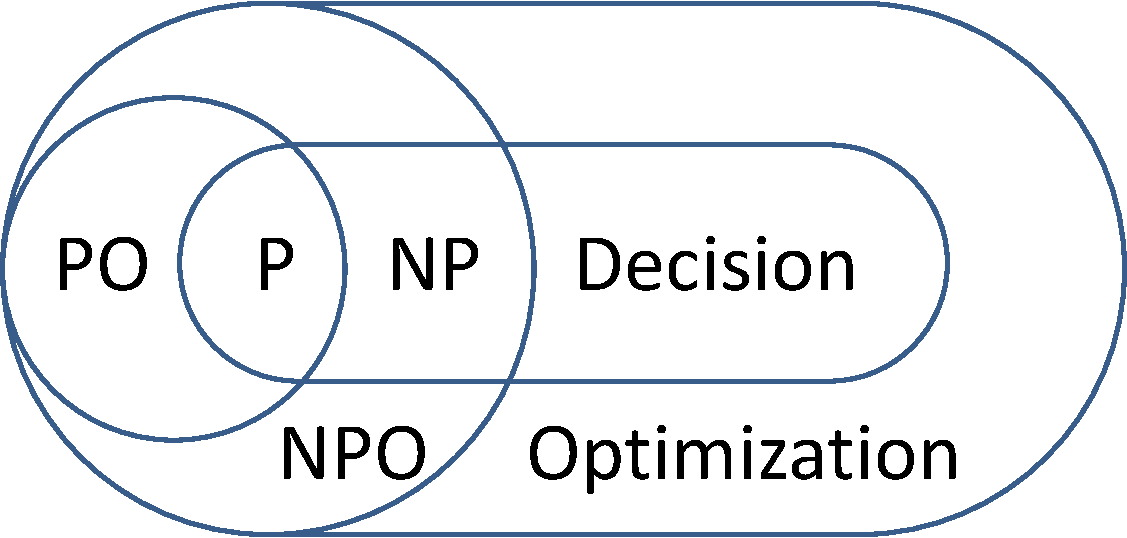
\includegraphics[width=0.43\linewidth]{figure/Classes-P-NP-crop.pdf}\end{tabular}%
% \ \ 
% 	 \begin{tabular}{c}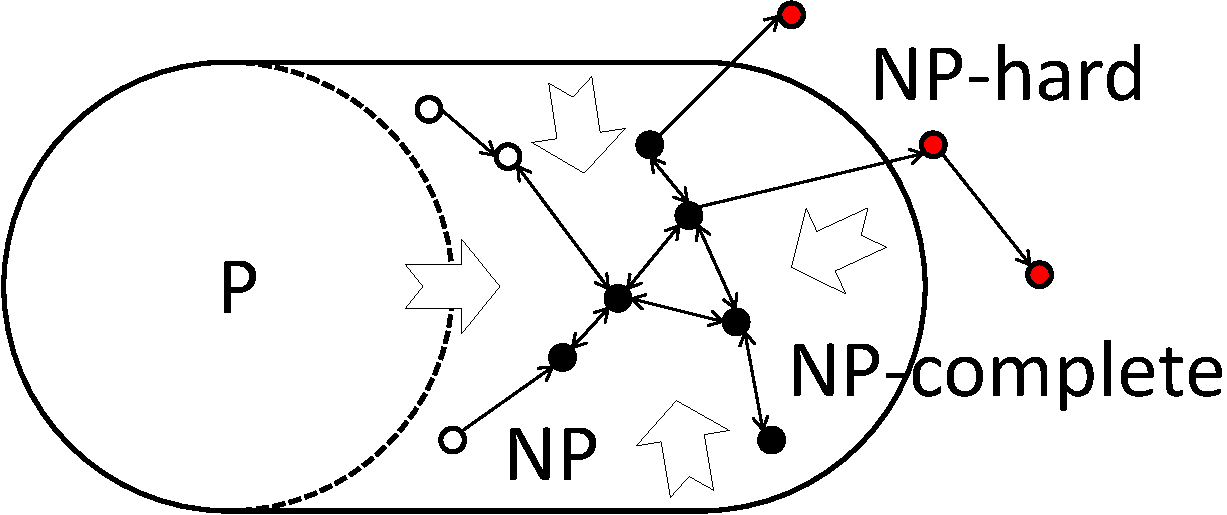
\includegraphics[width=0.5\linewidth]{figure/Classes-NP-hard-crop.pdf}\\[5pt]
% 	\end{tabular}%
% 	\end{tabular}
% 	}
% \end{center}
%   \caption{Left: relation of complexity classes between decision and optimization problems. Optimization problems ``contain'' decision problems since any decision problem can be cast as an optimization over the set $\{$yes, no$\}$. If not clear from the picture, P $\subseteq$ NP, P $\subseteq$ PO and NP $\subseteq$ NPO. Right: arrows indicate that a problem can be reduced to other problem in polynomial time. %All NP problems can be reduced to NP-complete problems. If a problem is such that an NP-complete problem reduces to it, 
% % I am not sure you need to include the right part of the figure.  Anyone reading the paper should understand the basic concept of a reduction.
% NP-hard class contains NP-complete problems and all problems (not necessarily decision) that are at least as hard (to which an NP-complete problem, and thus all problems in NP, may be reduced).
% }
% \label{fig:Classes-P-NP}
% \end{figure}

Suggestions for the right part figure 2 (update: already merged with figure 1 now):

Three ways to improve it:

1. Keep the idea of using dots as problems and edges as reductions, but makes solid arrows larger and replace hollow arrows with a dotted boundary for NP-complete problems.

2. Actually, wikipedia has a nice figure explaining this problem:
\par
\url{https://en.wikipedia.org/wiki/P_versus_NP_problem#/media/File:P_np_np-complete_np-hard.svg}
\par
We don't need to introduce reduction here for a) simplicity, b) avoid technical issues:
Karp reduction is used for reductions among decision problems while Turing reduction is used from decision problems to optimization problems. In other words, the typical reduction used for decision problems does not work for optimizaiton problems.

3. Just remove the right half of figure 2 as it is already something well explained on Wikipedia. We can resort to just text explanation.

---------------------------------------





   %Discrete energy minimization is an established work engine for performing inference in graphical models 
%   Discrete energy minimization is a recognized optimization problem, used to solve MAP inference in graphical models and closely related to several well-known combinatorial optimization problems.
%<<<<<<< Updated upstream
   %In this paper we give a comprehensive overview of subclasses solvable in polynomial time as well as subclasses admitting a constant factor approximation. We further contribute to the study of complexity by showing that general energy minimization is exp-APX-complete, meaning it is as hard as any optimization problem with a polynomial-time computable objective function and whose arbitrary feasible solution can be found in polynomial time, and the general problem cannot be approximated with a better then exponential factor. The result holds already in case of two labels, \ie, for quadratic pseudo-Boolean optimization. Further, we show that planar problem with 3 labels is exp-APX-complete as well.
%% \par
% \revisit[I think it might be better to keep the exponential factor as in previous version. "as hard as bla bla" is still vague to people without a sense of what is an optimization problem.]
%=======
%   In this paper we give a comprehensive overview of subclasses solvable in polynomial time as well as subclasses admitting a constant factor approximation. We further contribute to the study of complexity by showing that general energy minimization is exp-APX-complete, meaning that 
% 	it is NP-hard to approximate it with a subexponential ratio. %find a solution with energy within a subexponential (in the problem size) factor of the minimum.
%  %and cannot be approximated with a better then exponential factor. 
% The result holds already in case of two labels, \ie, for quadratic pseudo-Boolean optimization. Further, we show that planar problem with 3 labels is exp-APX-complete as well.
% \par
% %\revisit[I think it might be better to keep the exponential factor as in previous version. "as hard as bla bla" is still vague to people without a sense of what is an optimization problem.]
% %>>>>>>> Stashed changes
     
% \revisit[See ideas.tex for an alternative abstract that is tied closer to computer vision]


% Discrete energy minimization problem, which can be used to solve MAP inference for graphical models, is widely adopted in computer vision and machine learning. Despite many subclass problems are identified as NP-hard, they are still used to model real world applications. In this paper, we present a comprehensive overview of the computational complexity of subclass problems by arranging them on a finer complexity scale consisting of three major complexity classes --- PO, APX, exp-APX, corresponding to problems that are solvable, approximable, inapproximable in polynomially time. The connections of these subclass problems will also be analyzed. We hope this overview will aid researchers in designing new optimization algorithms
% and in selecting appropriate models for their applications. Moreover, we contribute two important additions to this overview by showing that general energy minimization and planar 3-label energy minimization are exp-APX-complete. This essentially mean that there cannot be any approximation algorithm with an approximation ratio better than an exponential function in the input size for these two problems. Therefore algorithm designers should not expect to prove a reasonable approximation ratio guarantee for their algorithms on these problems.


---------------------------

Previous version of the related works:


% NP-hardness has been shown for the MAP assignment of belief networks by~\citet{Cooper-90} and \citet{Shimony-94}. \citet{Abdelbar-98} has shown that approximating the MAP assignment is also NP-hard. However, there are substantial differences from our result.
% Belief networks have a probability density function $p(x)$ that factors according to a directed acyclic graph, \eg, as $p(x_1,x_2,x_3) = p(x_1 | x_2,x_3)p(x_2)p(x_3)$. %Using the relation $p(x) = \exp(-f(x))$, 
% %The negative logarithm of the pdf is then representable as a partially separable function of the form~\eqref{eq:1}. Maximization of the probability 
% For belief networks, finding the MAP assignment\footnote{Same as the most probable estimate (MPE).} in a Bayesian network is related to energy minimization~\eqref{eq:1} by letting $f(x) = -\log(p(x))$. The product is transformed into the sum and so, \eg, factor $p(x_1 | x_2,x_3)$ corresponds to term $f_{1,2,3}(x_1,x_2,x_3)$.
% %
% Note, factors of at most two variables, \eg, $p(x_1 | x_2)$, can form only a tree-structured model. % and therefore a Bayesian Network corresponding to a given energy may require higher order factors.
% %In the other direction, 
% Therefore, a Bayesian network corresponding to the pairwise energy~\eqref{eq:1} may require to use factors of order up to $|V|$. \revisit[this sentence is confusing] % in the Bayesian Network representation. 
% It is seen that while the general problems are convertible, fixed-parameter classes (such as order and graph restrictions) differ. In addition, approximation ratio for probabilities translates to an absolute approximation (an additive bound) for energies.


% \citet{Abdelbar-98} has shown that approximating the MAP assignment is also NP-hard. However, there are substantial differences from our result.

% are two neccessary conditions for the problem to be in PO. 
% more general means not only undirected graphical models,
% not only MAP inference, also marginal, partition function

% how to properly cite this?
% http://www.cs.huji.ac.il/project/PASCAL/index.php

% It is well-known that QPBO is NP-hard, since it generalizes such problems as maximum cut and maximum 2-satisfiability~\cite{Karp-72}. 
% These problems are also known to be APX-complete~\cite{Papadimitriou-91} (implies NP-hardness). Therefore, QPBO is APX-hard.
% %::: this does not flow very well.  This next text is not really related work.  It is more about our work.  Maybe better to just say "In this paper, we prove the stronger claim that QPBO is complete in exp-APX."
% Completeness in exp-APX is stronger. 
%::: suggest moving the following text to the section on the proof.
% In particular, it shows that such problems as general traveling salesman problem (TSP) can be reduced to QPBO while preserving approximation ratio in a linear fashion.

%:::\revisit[Consider finding a place to explicitly stating that BNs capture different families of distributions than energy minimization and thus they are used to model different problems]

% NP-hardness has been shown for the MAP assignment of belief networks by~\citet{Cooper-90} and \citet{Shimony-94}. \citet{Abdelbar-98} has shown that approximating the MAP assignment is also NP-hard. However, there are substantial differences from our result.
% Belief networks have a probability density function $p(x)$ that factors according to a directed acyclic graph, \eg, as $p(x_1,x_2,x_3) = p(x_1 | x_2,x_3)p(x_2)p(x_3)$. %Using the relation $p(x) = \exp(-f(x))$, 
% %The negative logarithm of the pdf is then representable as a partially separable function of the form~\eqref{eq:1}. Maximization of the probability 
% For belief networks, finding the MAP assignment\footnote{Same as the most probable estimate (MPE).} in a Bayesian network is related to energy minimization~\eqref{eq:1} by letting $f(x) = -\log(p(x))$. The product is transformed into the sum and so, \eg, factor $p(x_1 | x_2,x_3)$ corresponds to term $f_{1,2,3}(x_1,x_2,x_3)$.
% %
% Note, factors of at most two variables, \eg, $p(x_1 | x_2)$, can form only a tree-structured model. % and therefore a Bayesian Network corresponding to a given energy may require higher order factors.
% %In the other direction, 
% Therefore, a Bayesian network corresponding to the pairwise energy~\eqref{eq:1} may require to use factors of order up to $|V|$. \revisit[this sentence is confusing] % in the Bayesian Network representation. 
% It is seen that while the general problems are convertible, fixed-parameter classes (such as order and graph restrictions) differ. In addition, approximation ratio for probabilities translates to an absolute approximation (an additive bound) for energies.
% %Matching the pairwise model~\eqref{eq:1} is not possible unless the Bayesian network is a chain. 
% %It is not possible to end up with a pairwise model~\eqref{eq:1} unless the Bayesian network is a chain. 
% %The factorization can be regarded as a Gibbs distribution, with the same factors.
% %When written as a Gibbs distribution, the order of the factors (the number of variables involved)
% \par
% \citet{Abdelbar-98} has shown that approximating the MAP assignment in the value of probability, \ie, finding $x$ such that
% \begin{align}\label{p-approx-ratio}
% \frac{p(x^*)}{p(x)} \leq r(n)
% \end{align}
% with a constant or polynomial ratio $r(n) \geq 1$ is NP-hard, showing that this problem is poly-APX-hard. 
% This result holds even after restricting to binary variables and factors of order 3.\footnote{\citet[\parSym 6.1]{Abdelbar-98} count incoming edges of the network: for a factor $p(x_1 | x_2,x_3)$ there are two, but the total number of variables it couples is 3.} In addition they showed that the following problems are also APX-hard:
% \begin{itemize}
% \item knowing the optimal solution, approximate the next optimal solution;
% \item knowing the optimal solution, approximate the optimal solution conditioned on a changed assignment of one variable. 
% \end{itemize}
% %The difference to our result is that approximation ration for MPE translates to additive approximation of energies (in order to translate a multiplicative factorization of a Belief Network to an additive one of the form~\eqref{eq:1}, the connection should be given by $p(x) = \exp(-E(x))$). 
% %Additionally, their proof was given for a model involving four-tuple interactions (three-tuple in case of~\cite[\parSym 6.1]{Abdelbar-98}), and in this respect ours is a refinement. 
% %We also imply a stronger hardness: while \cite{Abdelbar-98} shows it is NP-hard to approximate with a polynomial factor, we show it is NP-hard to approximate with a subexponential factor.
% However, \eqref{p-approx-ratio} translates to an absolute energy approximation with a bound of $\log (r(n))$, \ie, logarithmic in $n$. We will show as a corollary from our result that it provides a stronger inapproximability for probabilities. % than poly-APX-hard.
% %We will show as a corollary from our result that approximating in the value of probability is exp-APX-complete as well, which in particular implies the problem is poly-APX-hard.
% \par
% \citet{Kwisthout-11} showed NP-hardness of absolute approximation in the value of probability for MAP in Bayesian networks, and also studied different approximation measures: structure- rank- and expectation approximations and has established similar inapproximability results for them~\cite{Kwisthout-13}.
% %that is it NP-hard to find a solution $x$ such that 
% %$p(x) \geq p(x^*) - \rho$
% %that additive $\pro$-approximation of MAP is NP-hard for $\rho \geq > $.
% % \par
% % \revisit How additive approximation relates to multiplicative. Does our result implies \citet{Abdelbar-98} or other way around?

% %also that finding an approximate solution with the value of posteriori probability by at most  solution is NP-hard as well.
% %\citet{Abdelbar-98} has shown 

% %Work on stating the inference is NP-hard

% % Work on investigating the hardness of the problem from approximation perspective

% % Work on establishing complexity scales, i.e. by reductions other than AP-reduction.



% \newpage
% \let\authcount\relax
% \tableofcontents

\end{document}
